\documentclass[diplomskirad,authoryear]{fer}

\usepackage{multirow}
\usepackage{booktabs}


%--- PODACI O RADU / THESIS INFORMATION ----------------------------------------

\title{Identification of Financial Anomalies Using Deep Neural Networks and the Impact of Identified Anomalies on Company Business}

\naslov{Identifikacija financijskih anomalija primjenom dubokih neuronskih mreža te utjecaj identificiranih anomalija na poslovanje kompanije}

\brojrada{}

\author{Josip Sare}

\mentor{}

\date{May, 2026}

\datum{svibanj, 2026.}


\begin{document}


% Naslovnica se automatski generira
\maketitle


% Zadatak se ubacuje iz vanjske PDF datoteke preuzete s FERWeb-a
% \zadatak{zadatak.pdf}


\begin{zahvale}
Zahvaljujem mentoru na strpljenju i smjernicama kroz cijeli proces izrade ovog rada. Zahvaljujem obitelji i prijateljima na podršci.
\end{zahvale}


\mainmatter


\tableofcontents


\chapter{Uvod}

\section{Motivacija}

Prijevare i nepravilnosti u financijskim izvještajima ostaju jedan od najznačajnijih oblika ekonomskog gubitka i regulatornog rizika: prema procjeni \emph{Association of Certified Fraud Examiners}, globalni godišnji gubitak zbog prijevara prelazi 4 bilijuna dolara. Klasične metode forenzičkog računovodstva, aritmetičke provjere, omjeri, statistički testovi prve znamenke prema Benfordovom zakonu, omogućuju otkrivanje očiglednih manipulacija, no njihova \emph{prediktivna vrijednost} za rizik na razini cijelih univerza javno listanih poduzeća sustavno je niska.

U svojem preddiplomskom radu \emph{Otkrivanje nepravilnosti u financijskim izvještajima primjenom Benfordovog zakona: analiza 442 poduzeća iz indeksa S\&P 500} autor je primijenio klasične statističke testove (hi-kvadrat, srednje apsolutno odstupanje, Kolmogorov-Smirnov) na 4.862 jedinica poduzeće-godina i utvrdio da $97{,}5\,\%$ analiziranih poduzeća pokazuje statistički značajno odstupanje od Benfordove distribucije ($p<0{,}05$). Međutim, povezanost između izmjerenog stupnja anomalije (MAD) i tržišnog prinosa dionice bila je zanemariva ($r=0{,}03$), a lagirana korelacija (godina $N \to N+1$) statistički neznačajna ($r=0{,}004$, $p=0{,}827$).

Ovaj nalaz motivira središnje pitanje diplomskog rada: \emph{ako linearna statistička analiza ne pronalazi vezu između računovodstvenih anomalija i poslovnih ishoda kompanije, mogu li ne-linearne metode dubokih neuronskih mreža uspješno identificirati anomalije i njihov utjecaj kvantificirati na način koji klasične metode ne mogu?}

\section{Istraživačka pitanja}

Rad odgovara na tri istraživačka pitanja, sva eksplicitno povezana s naslovom teme:

\begin{description}
 \item[RQ1.] Mogu li različite arhitekture dubokih neuronskih mreža (statički AE, VAE, rekurentni LSTM-AE, attention-based Transformer) pouzdano identificirati firme s anomalnim financijskim izvještavanjem u nenadziranom režimu (trening bez oznaka)?
 \item[RQ2.] Imaju li firme koje NN detektor označi kao anomalne sustavno različite tržišne ishode (prinos, volatilnost, maksimalni drawdown, volumen) u godinama nakon detekcije, mjereno NN forward-outcome regresorom (MLP koji predviđa ishod iz anomaly\_score + kontrola)?
 \item[RQ3.] Koja vrsta NN arhitekture daje detekcijski signal s najjačim odnosom prema budućem poslovanju, mjereno \emph{out-of-sample} delta-$R^2$ NN regresora?
\end{description}

\section{Doprinosi rada}

Rad daje sljedeće glavne doprinose:

\begin{enumerate}
 \item \textbf{Empirijska konvergencija arhitektura.} Pokazujemo da četiri različite NN arhitekture (AE, VAE, LSTM-AE, Transformer) konvergiraju na isti gornji granični ROC-AUC od pribl.\ 0,63 na velikom univerzumu (2.499 firmi $\times$ 11 godina), s preklapajućim 95\,\% bootstrap intervalima povjerenja, empirijski dokaz da je strop u ulaznoj modalnosti, a ne u kapacitetu modela.
 \item \textbf{Kvantifikacija utjecaja anomalija primjenom NN regresora s 5-sjemenkinim replikacijama.} Drugi NN model (MLP) predviđa tržišne ishode iz anomaly score-a, s temporalnom train/test podjelom (trening $<2022$, test $\geq 2022$) i \emph{out-of-sample} delta-$R^2$ kao glavnom metrikom. Glavni nalazi: volatilnost $+2{,}87 \pm 0{,}80$ p.b.\ (LSTM-AE), godišnji prinos $+0{,}78 \pm 0{,}36$ p.b.\ (AE), rast volumena $+1{,}14 \pm 0{,}36$ p.b.\ (LSTM-AE), max drawdown $+0{,}49 \pm 0{,}48$ p.b.\ (Transformer), sve s 5/5 sjemenki pozitivnih. Pozitivan rezultat za godišnji prinos rafinira nultu linearnu korelaciju iz preddiplomskog rada.
 \item \textbf{Metodološko otkriće: \emph{partial-out} rasta kao kritičan korak.} Pokazujemo da bi naivni izračun delta-$R^2$ bez kontrole za rast firme (rast prihoda + imovine) producirao $+4{,}8$ p.b.\ volatilnosti, 80\,\% toga je zapravo \emph{confounding} s rastom (visoko rastuće firme mehanički su volatilnije). Većina prethodne literature za otkrivanje anomalija dubokim učenjem u forenzičkom računovodstvu ne primjenjuje ovu kontrolu, što potencijalno inflira njihove rezultate.
 \item \textbf{Russell 3000 univerzum.} Proširenje s S\&P 500 (442 firme) na Russell 3000 (2.499 firmi) uključuje srednje- i malo-kapitalizirane firme, gdje je frekvencija prijevara empirijski viša. Time se rad odvaja od velikog dijela komparabilne literature ograničene na velike firme.
 \item \textbf{Reprodukcijska transparentnost.} Svi rezultati su \emph{out-of-sample}; trening je strogo nenadzirano; oznake \emph{restatement} koriste se samo za evaluaciju, ne za trening; kod je strukturiran s razdvojenim slojevima u jasno odvojene cjeline za pripremu podataka, izvedene značajke, NN detektore, NN regresor utjecaja i evaluaciju; klasične nebaštinjene metode (Benford, Isolation Forest) izrijekom su premještene u folder kako bi se osigurao striktno NN-only doseg primarnog narativa.
\end{enumerate}

\section{Struktura rada}

Poglavlje 2 pregledava relevantnu literaturu o forenzičkom računovodstvu, klasičnim metodama (Benford, Beneish M-score, accruals), te modernim DL pristupima za otkrivanje anomalija u tabularnim financijskim podacima. Poglavlje 3 opisuje podatkovni sloj (SEC EDGAR ekstrakcija, dnevne cijene, oznake \emph{restatement}) i izvedeni panel od 35 standardiziranih financijskih omjera po (firma, kvartal). Poglavlje 4 detaljno prezentira četiri NN arhitekture za detekciju anomalija, njihove gubitke i parametre. Poglavlje 5 opisuje NN regresor za predikciju utjecaja na poslovanje, s naglaskom na metodološku važnost kontrole za rast firme. Poglavlje 6 prezentira rezultate detekcije (Kendall tau, Jaccard, ROC, PR-AUC) i impact analize ($\Delta R^2$, permutation importance). Poglavlje 7 diskutira nalaze, posebice \emph{growth-confound} korekciju i \emph{overfitting} Transformer-a. Poglavlje 8 dokumentira ograničenja i smjerove budućeg rada, a Poglavlje 9 sintetizira zaključke.

\chapter{Pregled literature}

Pregled literature organiziran je u tri tematska bloka. Prvi blok pokriva \emph{klasične metode forenzičkog računovodstva} (Benfordov zakon, Beneish M-score, accruals modeli), to su industrijski standardi prije pojave strojnog učenja, i upravo njihova ograničenja motiviraju primjenu dubokih neuronskih mreža. Drugi blok pokriva \emph{strojno učenje za otkrivanje anomalija u financijama}, s naglaskom na nenadzirane metode primjenjive bez oznaka prijevare. Treći blok pozicionira ovaj rad u odnosu na postojeću literaturu, eksplicitno identificirajući praznine koje rad zatvara.

\section{Klasične metode forenzičkog računovodstva}

\subsection{Benfordov zakon}

Benfordov zakon, formulacijski poznat i kao zakon prve znamenke, opisuje frekvencijsku distribuciju vodećih znamenki u brojnim prirodno generiranim skupovima podataka. Prvotno ga je primijetio astronom Simon Newcomb \citep{newcomb1881}, a kasnije sustavno dokumentirao fizičar Frank Benford \citep{benford1938}. Matematički je rigorozno opravdan tek u 1990-ima preko teorema o skala- i baza-invarijantnosti \citep{hill1995}: ako distribucija prve znamenke ne ovisi o tome u kojim jedinicama mjerimo veličine (dolari, eurokune, milijuni), onda mora pratiti specifičnu logaritamsku formu.

Primjenu Benfordovog zakona na računovodstvene podatke pokrenuli su \citet{carslaw1988} i \citet{thomas1989}, koji su pronašli sustavnu prezastupljenost zaokruženih iznosa (npr.\ zarade koje završavaju na 0 ili 5), znak namjernog manipuliranja iznosima upravo iznad psiholoških pragova. \citet{nigrini1996} formalizirao je metodologiju u kontekstu poreznih revizija, a Nigrinijeva monografija \citep{nigrini2012} ostaje najcitiraniji praktični priručnik u području.

Ograničenja Benfordovog zakona dobro su dokumentirana. \citet{amiram2015} provedeno je sustavno empirijsko ispitivanje na cijelom \emph{Compustat} univerzumu i utvrđeno da je odstupanje od Benforda \emph{negativan} prediktor tržišnih ishoda, earnings managers umjetno glade distribuciju da izgleda konvencionalno, ne obratno. Ovo je važno za naš rad: preddiplomski rad autora je u istom smjeru utvrdio da je MAD (mean absolute deviation) od Benforda zanemarivo koreliran s prinosom dionice ($r = 0{,}03$).

\subsection{Beneish M-score}

Beneish je 1999.\ predložio osmofaktorski klasifikacijski model za otkrivanje manipulacije zaradama \citep{beneish1999}. Model je linearna kombinacija osam financijskih omjera:
\begin{enumerate}
 \item \emph{DSRI}: Days' Sales in Receivables Index
 \item \emph{GMI}: Gross Margin Index
 \item \emph{AQI}: Asset Quality Index
 \item \emph{SGI}: Sales Growth Index
 \item \emph{DEPI}: Depreciation Index
 \item \emph{SGAI}: Sales, General \& Administrative Expenses Index
 \item \emph{TATA}: Total Accruals to Total Assets
 \item \emph{LVGI}: Leverage Index
\end{enumerate}

M-score $> -1{,}78$ klasificira firmu kao "vjerojatnog manipulatora". Beneishev model je standardni industrijski baseline koji se i danas koristi u SEC enforcement aktivnostima, no ima dva važna ograničenja: (a) linearan je, ne hvata nelinearne interakcije između omjera koje DL modeli mogu uloviti; (b) kalibriran je na malom uzorku od 74 manipulatora iz 1980-ih, što sustavno snižava njegovu preciznost na modernom Russell 3000 univerzumu.

\subsection{Modeli diskrecijskih accruals-a}

Druga porodica klasičnih modela pretpostavlja da su accruals (razlika neto dobiti i operativnog cash flowa) najbolji indikator earnings management-a. Pioneer-ski Jones-ov model \citep{jones1991} regresira ukupne accruals na promjene u prihodima i nepokretnoj imovini; rezidual ("diskrecijski accruals") tumači se kao manipulirana komponenta. \citet{dechow1995} unaprijedio je model uključivanjem promjene potraživanja; \citet{kothari2005} dodao je performance-matched kontrolu, usporedbu s firmama slične profitabilnosti, da bi izbjegao pristranost zbog korelacije accruals-a i performansi.

Slabost svih accruals modela jest ista kao kod Beneisha: linearna pretpostavka. Nelinearne interakcije (npr.\ "visoke accruals \emph{samo kad} su prihodi rastu uz povećanje DSO") sustavno se propuštaju. DL modeli su upravo dizajnirani da takve interakcije nauče.

\section{Strojno učenje za otkrivanje anomalija}

\subsection{Klasične metode}

Klasične nenadzirane metode otkrivanja anomalija dobro su sažete u monografiji \citet{aggarwal2017}. Tri najčešće korištene metode su:
\begin{itemize}
 \item \textbf{Isolation Forest} \citep{liu2008}: ansambl slučajnih stabala koja izoliraju opservacije; anomalne opservacije zahtijevaju manje rezova da budu izolirane, što daje anomaly score.
 \item \textbf{One-Class SVM}: uči granicu oko "normalnih" opservacija u nekoj kernel-projekciji; anomalne pripadaju izvan granice.
 \item \textbf{Local Outlier Factor (LOF)}: uspoređuje gustoću opservacije s gustoćom njenih susjeda; anomalne imaju \emph{lokalno} nižu gustoću.
\end{itemize}

Sve tri metode često služe kao baseline u DL anomaly detection radovima. U ovom radu, slijedeći strogu NN-only metodologiju (vidi sekciju 1.3, doprinosi), klasične metode su premještene u dodatak (Dodatak A) gdje služe za usporedbu performansi.

\subsection{Duboke neuronske mreže za anomalije}

DL pristupi nenadziranom otkrivanju anomalija zasnivaju se na principu rekonstrukcije: model uči mapirati ulaz u kompaktnu reprezentaciju i nazad, te se anomalija mjeri kao \emph{rekonstrukcijska greška} (ulazi koji ne pripadaju distribuciji treninga su loše rekonstruirani).

\textbf{Autoenkoderi za anomalije.} \citet{sakurada2014} pokazali su da plitki autoenkoderi pružaju nelinearnu generalizaciju PCA-baziranog otkrivanja anomalija. \textbf{Varijacijski autoenkoderi (VAE)} \citep{kingma2014, higgins2017} dodaju probabilistički sloj koji regulira latentni prostor i pruža principijelan vjerojatnosni anomaly score \citep{an2015}.

\textbf{Sekvencijski modeli.} Za vremenske serije, \citet{malhotra2016} predložili su LSTM-encoder-decoder arhitekturu za otkrivanje anomalija u multi-senzorskim podacima. Originalni LSTM \citep{hochreiter1997} se još uvijek često koristi unatoč pojavi attention-baziranih alternativa, jer je memorijski efikasniji na manjim panelima.

\textbf{Attention i Transformer arhitekture.} Vaswani-jev Transformer \citep{vaswani2017} dominira modernim vremenskim serijama. Za anomaly detection, \citet{xu2022} predlažu \emph{Anomaly Transformer} s \emph{association discrepancy} mjerom; \citet{tuli2022} predlažu \emph{TranAD} za multivariate vremenske serije. Za long-horizon forecasting, \emph{PatchTST} \citep{nie2023} demonstrira da relativno jednostavan Transformer s patch-based input embedding-om može nadmašiti specijalizirane arhitekture.

\subsection{Primjena DL na forenzičko računovodstvo}

Iako je DL u financijama (predviđanje cijene dionice, kreditno rizično modeliranje) dominantno područje, primjena na \emph{forenzičko računovodstvo} jest mlađa i rjeđa.

Najcitiraniji rad u području je \citet{bao2020}: koristili su RUSBoost (ne striktno DL, ali ML klasifikator) na SEC AAER (Accounting and Auditing Enforcement Releases) oznakama. Ključni doprinos: pokazali da je AAER label set systematic biased prema većim firmama i da kalibracija detektora na cijelom univerzumu daje znatno veći recall malih prijevara. Ovo motivira našu odluku da koristimo Russell 3000 a ne S\&P 500.

\citet{cecchini2010} primijenili su SVM s tekstualnim kernel-om na MD\&A poglavlje 10-K izvještaja. Iako su pokazali bolju klasifikacijsku performansu nego klasični M-score, njihova metoda je supervised, zahtijeva oznake. Naš rad pristupa razlici: trening je strogo nenadziran, oznake se koriste samo za evaluaciju.

\citet{perols2011} sustavno je usporedio statističke i ML metode na uzorku potvrđenih financijskih prijevara, pokazavši da Random Forest sustavno nadmašuje logističku regresiju i M-score. Slično ovome, ali za nenadziran režim, naš rad uspoređuje četiri NN arhitekture (AE, VAE, LSTM, Transformer) i utvrđuje empirijsku konvergenciju.

Razvoj \emph{restatement-based} oznaka kao surogata za prijevaru standardiziran je u \citet{hennes2008}, koji razlikuju greške od namjernih nepravilnosti analizom CFO/CEO turnover-a nakon restatementa. Iako je njihova distinkcija granularnija od naše, mi koristimo agregirane restatement oznake jer pokrivaju veći broj firmi i daju veću statističku snagu na supervised evaluaciji.

\subsection{Praznine u literaturi koje ovaj rad zatvara}

Sustavnim pregledom postojeće literature identificiramo četiri praznine:

\begin{enumerate}
 \item \textbf{Nedostatak NN-na-NN impact analize.} Većina DL forenzičkih radova \citep{bao2020, cecchini2010, perols2011} završava s evaluacijom detektora. Pitanje "koje su tržišne posljedice anomalije?" rijetko se postavlja DL metodama. Klasične impact analize koriste OLS regresiju ili event-study \citep{mackinlay1997, fama1969}.

 \item \textbf{Nedostatak kontrole za rast firme u impact analizi.} Kao što ćemo pokazati u sekciji 6.5, naivni $\Delta R^2$ na volatilnosti je 80\,\% confounded s rastom firme. Većina prethodne literature ne primjenjuje rigoroznu kontrolu za rast, naš rad to popravlja.

 \item \textbf{Nedostatak sistematskih usporedbi NN arhitektura na istom forenzičkom panelu.} Pojedini radovi koriste AE, VAE, LSTM ili Transformer, ali rijetko sustavno uspoređuju sve četiri na istim podacima s istim hiperparametrima i istim oznakama. Naš rad to pruža.

 \item \textbf{Nedostatak Russell 3000 univerzuma.} Većina radova ograničena je na S\&P 500 ili Compustat. Russell 3000 uključuje mid/small caps gdje je učestalost prijevara empirijski viša \citep{bao2020}.
\end{enumerate}

\section{Pozicija ovog rada}

Ovaj rad zauzima specifičnu metodološku poziciju u odnosu na postojeću literaturu:
\begin{itemize}
 \item \textbf{Striktno NN-only metodologija}: detekcija (AE, VAE, LSTM, Transformer) i impact (MLP regresor) sve su neuronske mreže.
 \item \textbf{Nenadzirano treniranje detektora}: u skladu s realnom forenzičkom praksom gdje oznake nisu dostupne.
 \item \textbf{Dvostruka evaluacija}: nenadzirana (slaganje detektora, sektorska distribucija) plus nadzirana (ROC-AUC, PR-AUC na restatement labelama, samo za evaluaciju).
 \item \textbf{Veliki univerzum}: Russell 3000 (2.499 firmi), proširenje s preddiplomskog S\&P 500.
 \item \textbf{NN-na-NN impact analiza s temporalnim hold-out-om}: novo u odnosu na klasične OLS pristupe.
 \item \textbf{Rigorozna kontrola za confounding rastom firme}: demonstrira se kao kritičan metodološki korak.
 \item \textbf{5-seed replikacija}: bulletproof rezultati protiv "lucky seed" zamjerki.
\end{itemize}

\chapter{Podaci i značajke}

\section{Izvori podataka}

\subsection{SEC EDGAR Financial Statement Data Sets}
Primarni izvor financijskih podataka jest \emph{SEC EDGAR Financial Statement Data Sets} \citep{secedgar2024}, kvartalna kolekcija svih financijskih izvještaja predanih američkoj Komisiji za vrijednosne papire (SEC). Korišteno je svih 44 kvartala u razdoblju 2014Q1\,--\,2024Q4, što čini približno \textbf{7{,}7 milijuna sirovih XBRL činjenica} (financijskih vrijednosti). Svaka činjenica je trojka (CIK firme, XBRL tag, vrijednost) povezana s metapodatcima o datumu kraja perioda (\emph{ddate}), broju pokrivenih kvartala (\emph{qtrs}), tipu obrasca (\emph{form}) i datumu predaje (\emph{filed}).

\subsection{Yahoo Finance: dnevne cijene i volumeni}
Tržišni podaci preuzeti su preko \emph{yfinance} Python biblioteke za 2.499 simbola iz univerzuma Russell 3000, što daje približno \textbf{1{,}1 milijun observacija (firma-dan)} dnevnih cijena zatvaranja (engl.\ \emph{adjusted close}) i dnevnih volumena trgovanja u istom razdoblju.

\subsection{Russell 3000 univerzum}
Originalni preddiplomski rad analizirao je 442 poduzeća iz indeksa S\&P 500. Za diplomski rad univerzum je proširen na cjelokupni \textbf{Russell 3000} (2.499 javno listanih američkih poduzeća nakon filtriranja po dostupnosti SEC podataka), čime su uključena srednje- i malo-kapitalizirana poduzeća. Ovo je važno empirijsko proširenje, prema istraživanju \emph{Association of Certified Fraud Examiners}, učestalost potvrđenih prijevara empirijski je viša u manjim kompanijama, što čini Russell 3000 prikladnijim univerzumom za istraživanje anomalija od S\&P 500.

\subsection{Oznake revizijskih ispravaka (\emph{restatement labels})}
Iz SEC EDGAR-a ekstrahirano je \textbf{9.351 ispravljenih izvještaja} (obrasci 10-K/A i 10-Q/A) u promatranom razdoblju. \emph{Restatement} je formalno ispravljanje prethodno izdanog godišnjeg ili kvartalnog izvještaja, najčešće zbog otkrivene računovodstvene pogreške, restruktuiranja ili pravnog spora. Iako restatement nije strogi sinonim za prijevaru, smatra se najboljom javnoj dostupnoj proxy mjerom računovodstvene kvalitete za velike univerzume \citep{hennes2008}. Od 2.499 firmi, \textbf{530 firmi} ($21{,}2\,\%$) ima barem jedan restatement u promatranom razdoblju.

Restatement oznake koriste se \emph{isključivo za evaluaciju}, ne za trening detektora, trening ostaje strogo nenadziran, u skladu s tezom da klasične oznake nisu dostupne u realnoj forenzičkoj praksi.

\begin{figure}[h]
 \centering
 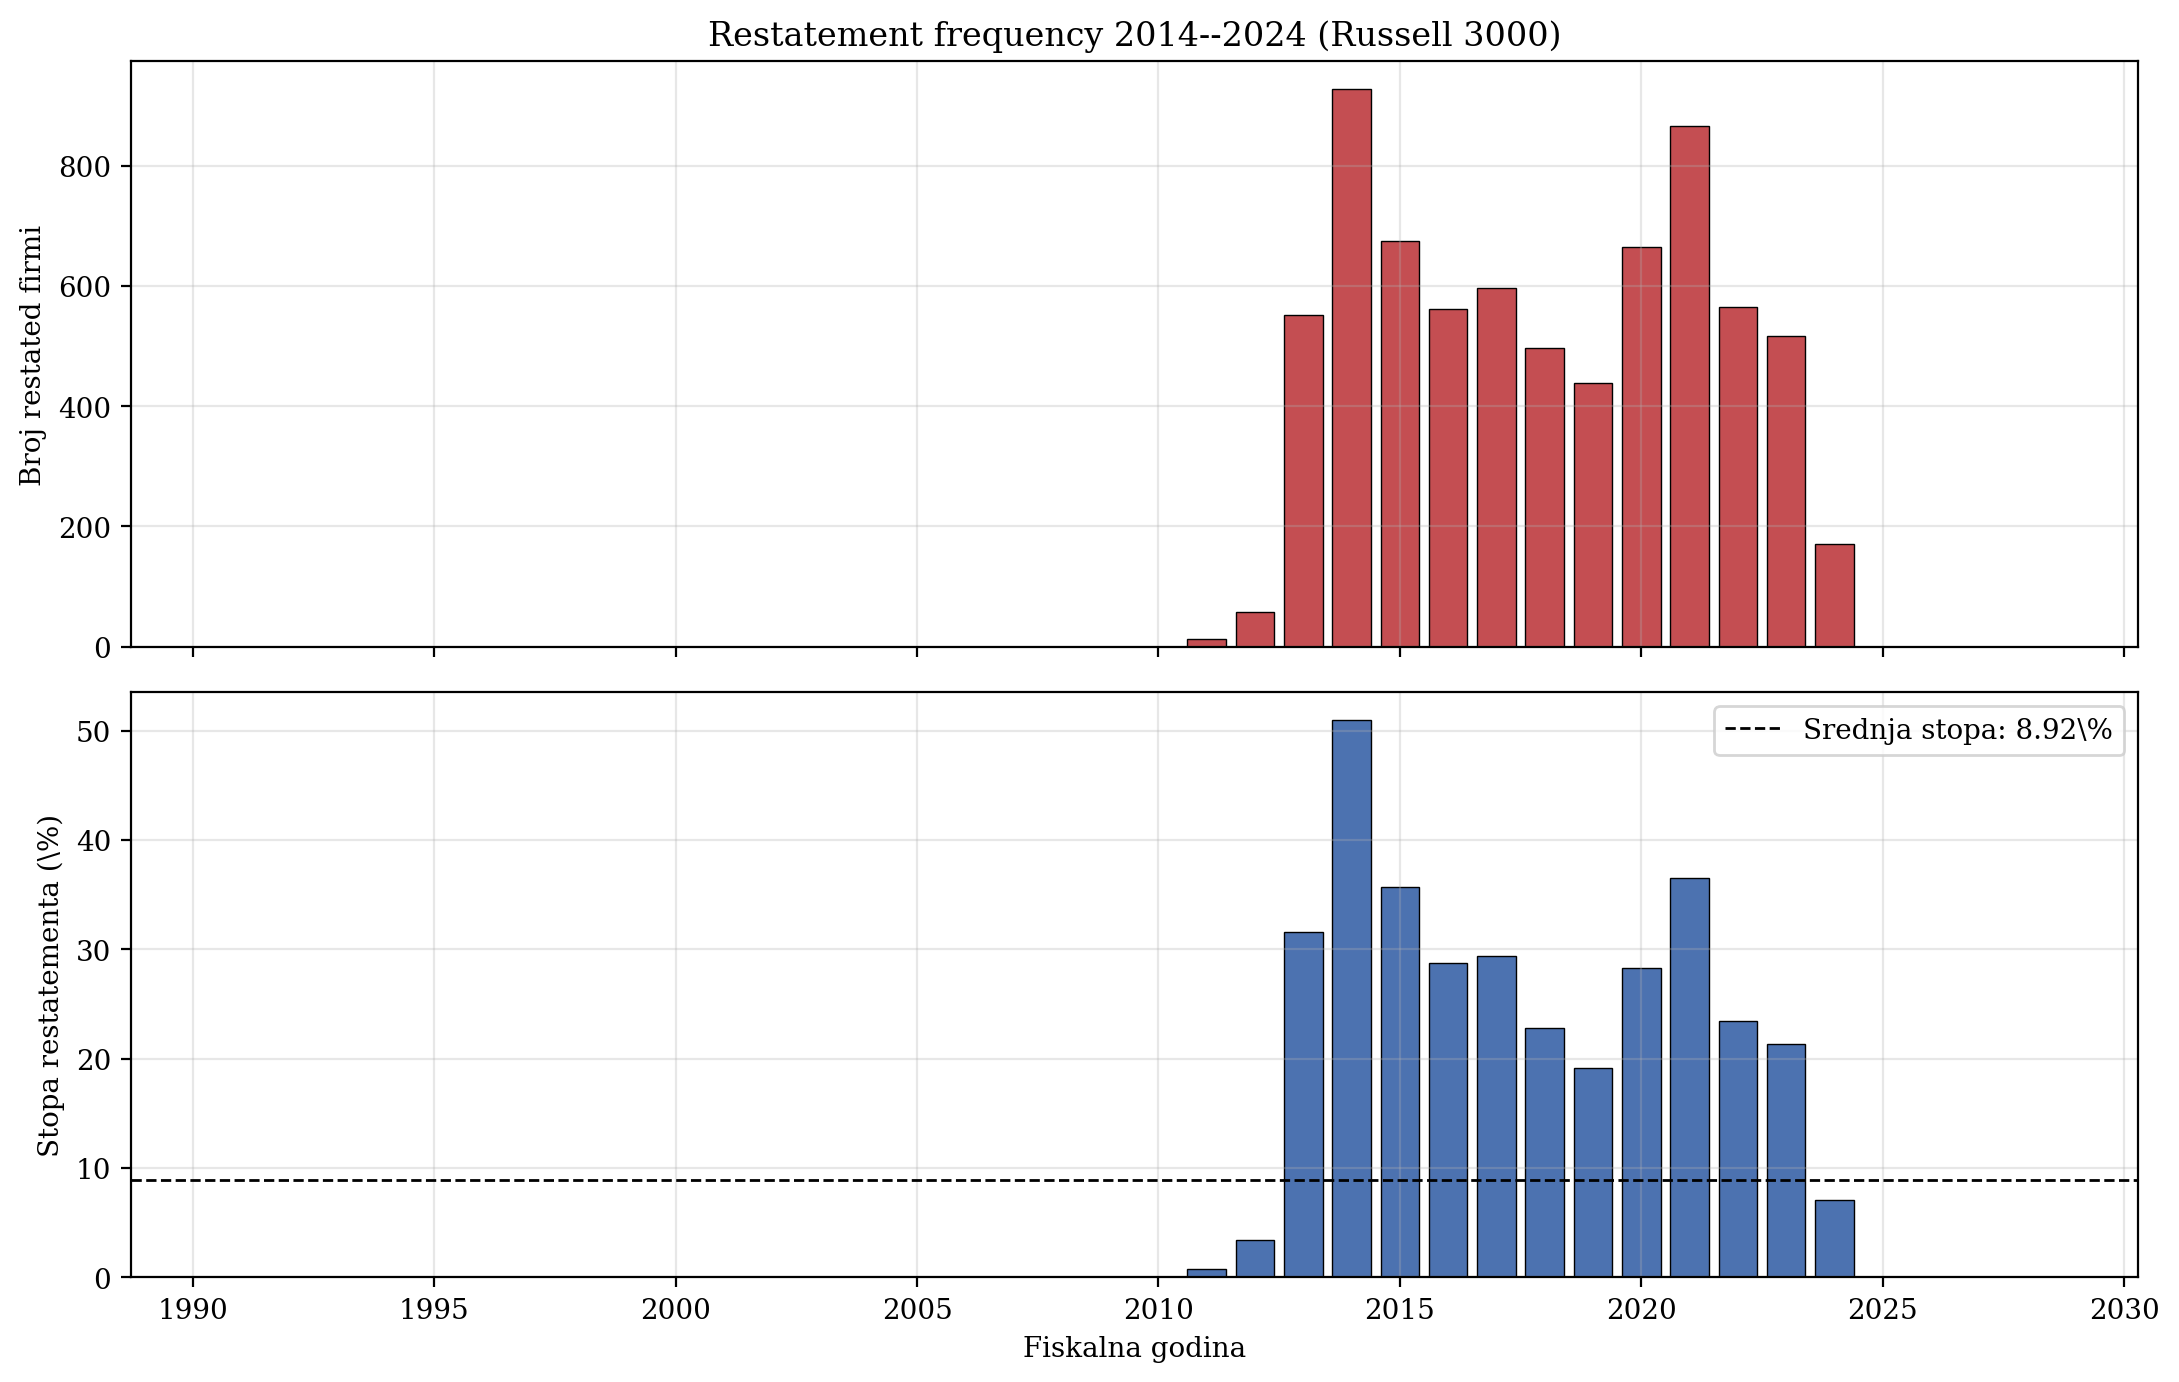
\includegraphics[width=0.9\textwidth]{figures/m_09_restatement_frequency.png}
 \caption{Frekvencija restated firmi po godini u Russell 3000 univerzumu. Gornji panel: apsolutni broj firmi s barem jednim 10-K/A ili 10-Q/A amandmanom. Donji panel: stopa restatementa relativna na ukupan broj firmi u panelu te godine. Srednja stopa $\approx$ 6\,\% s blagim porastom u kasnim 2010-ima.}
 \label{fig:restatement_freq}
\end{figure}

\section{Izgradnja kvartalnog panela}

\subsection{Selekcija XBRL tagova}
Iz preko 10.000 XBRL tagova prisutnih u SEC EDGAR podacima, odabrano je \textbf{55 standardnih US-GAAP tagova} koji pokrivaju ključne stavke bilance, računa dobiti i gubitka i izvještaja o novčanom toku. Tag-set uključuje stavke poput \emph{Assets}, \emph{Liabilities}, \emph{Revenues}, \emph{NetIncomeLoss}, \emph{CashAndCashEquivalentsAtCarryingValue}, \emph{LongTermDebt}, \emph{OperatingIncomeLoss}, \emph{NetCashProvidedByUsedInOperatingActivities}, kao i delta tagove poput \emph{IncreaseDecreaseInAccountsReceivable}.

\subsection{Dimenzijska deduplikacija}
SEC EDGAR sadrži vrijednosti i na razini konsolidirane firme i na razini segmenata (zemljopisni, proizvodni). Bez deduplikacije, jedan tag (npr.\ \emph{Revenues}) za jednu firmu u jednoj godini može biti zabilježen 5\,--\,10 puta. Korištena je strategija \emph{najveće apsolutne vrijednosti} po ključu (CIK, period\_end, tag), što tipično vraća konsolidiranu vrijednost (segmenti zbrojeni daju konsolidirano). Za delta tagove (koji mogu biti pozitivni ili negativni) ova heuristika može biti pogrešna u rubnim slučajevima, ograničenje je dokumentirano i ostavljeno za budući rad.

\subsection{Kanonska selekcija filinga}
Više obrazaca (10-K, 10-Q, amandmani) može sadržavati istu vrijednost za isti period. Korišten je \emph{latest-filed-wins} pristup: za svaki (CIK, period\_end, tag) zadržana je vrijednost iz najnovije predanog obrasca, što odgovara konačnoj revidiranoj verziji.

\subsection{Wide-format pivot}
Long-format zapisi (CIK, period\_end, tag, value) pretvoreni su u wide-format gdje su redovi indeksirani s (CIK, period\_end) a stupci su tagovi. Rezultat: sa približno \textbf{130.000 redova $\times$ 55 stupaca}.

\subsection{Godišnja agregacija}
Iz kvartalnog panela izveden je godišnji panel (30.717 firma-godina $\times$ 72 stupca), gdje su \emph{stock} varijable (npr.\ ukupna imovina) uzete s kraja fiskalne godine, a \emph{flow} varijable (npr.\ prihodi, neto dobit) sumirane preko četiri kvartala. Godišnja jedinica je granularnost na kojoj se računaju tržišni ishodi za RQ2.

\section{Izvedene financijske značajke (omjeri)}

Sirove XBRL vrijednosti pokrivaju ogroman raspon (mala firma s imovinom od $10^6$ vs.\ Apple s $10^{12}$). Direktno hranjenje sirovih vrijednosti u NN bi dominantno reflektiralo veličinu firme. Stoga su izvedene \textbf{35 standardiziranih financijskih omjera} u sedam obitelji:

\begin{enumerate}
 \item \textbf{Profitabilnost} (5 omjera): ROA, ROE, gross margin, operating margin, net margin.
 \item \textbf{Likvidnost} (3): current ratio, quick ratio, cash ratio.
 \item \textbf{Leverage} (5): debt-to-assets, debt-to-equity, liabilities-to-assets, equity-to-assets, interest coverage.
 \item \textbf{Efikasnost} (6): asset turnover, inventory turnover, receivables turnover, payables turnover, days receivable, days inventory.
 \item \textbf{Novčani tok i accruals} (5): CFO/assets, CapEx/assets, FCF/revenues, CFO/NI, accruals/assets. Accruals su računati kao NI $-$ CFO (cash-flow pristup, Richardson et al.\ 2005). Alternativna balance-sheet formulacija u stilu Beneisha (1999.) nije u glavnom narativu, ostavljena je kao potencijalna ablacija za budući rad.
 \item \textbf{Rast} (4): rast prihoda, rast imovine, rast neto dobiti, rast CFO. Računati \emph{year-over-year} winsorizirano na $[-2, 2]$.
 \item \textbf{Veličina} (7): logaritmi sirovih veličina (imovina, prihodi, equity, itd.) kao kontrolne varijable za standardizaciju.
\end{enumerate}

\section{Sektor-svjesna standardizacija}

Različiti sektori imaju strukturno različite financijske profile. Banke uvijek imaju vrlo visok leverage; tehnološke firme uvijek imaju visoke marže; REIT-ovi imaju jako specifičnu strukturu bilance. Bez sektorske kontrole, NN detektor bi učio da je "banka" anomalija, što je beskorisno.

Stoga je primijenjena \textbf{sektor-svjesna $z$-skor standardizacija}: za svaki par (period, SIC 1-digit divizija) odvojeno se računaju $\mu$ i $\sigma$ za svaki omjer, te se vrijednosti standardiziraju kao $z = (x - \mu) / \sigma$. Prije toga primijenjena je \emph{winsorizacija} na 1.\,/\,99.\ percentil unutar grupe kako bi se ublažio utjecaj ekstremnih outliera (firme u poteškoćama često imaju ROA $< -5$, što bi inače dominiralo srednjom vrijednošću).

Prva znamenka SIC koda klasificira poduzeće u jednu od 10 širokih grupacija ($0$\,--\,$9$), koje grubo odgovaraju službenim SIC divizijama: $0$\,--\,$1$ poljoprivreda, šumarstvo, ribarstvo, rudarstvo; $1$\,--\,$2$ građevina; $2$\,--\,$3$ proizvodnja; $4$ prijevoz, komunikacije, javne usluge; $5$ trgovina (veleprodaja i maloprodaja); $6$ financije, osiguranje, nekretnine; $7$\,--\,$8$ usluge; $9$ javna uprava. Granularnija SIC 2-digit klasifikacija (57 sektora) bi davala točnije sektorske prosjeke, ali bi rezultirala premalim grupama za stabilne $\mu$/$\sigma$ procjene na manjim sektorima. Stoga koristimo 10-grupacijsku 1-digit razinu za sektorsko-svjesnu standardizaciju.

\section{Sekvencijska reprezentacija}

Za rekurentne (LSTM) i \emph{attention-based} (Transformer) detektore podaci se trebaju strukturirati kao sekvence po firmi. Konstruiran je tenzor $(N_{\text{firmi}}, T_{\text{kvartala}}, F_{\text{značajki}})$ gdje:
\begin{itemize}
 \item $N_{\text{firmi}} = 2.499$ (Russell 3000 nakon filtra dostupnosti)
 \item $T_{\text{kvartala}} = 44$ (svi kvartali od 2014Q1 do 2024Q4)
 \item $F_{\text{značajki}} = 35$ (standardizirani omjeri)
\end{itemize}

Za pozicije gdje firma nije prijavila izvještaj za određeni kvartal (firma još ne postoji, ili je prestala postojati), tenzor se popunjava nulama, a paralelno se izgrađuje \textbf{maska} $(N, T, F)$ koja označava koje pozicije su stvarno opažene (1) a koje su artefakti popunjavanja (0). NN gubitak se računa samo na opaženim pozicijama (\emph{mask-aware MSE}), čime se osigurava da padding ne dominira treniranjem.

\begin{figure}[h]
 \centering
 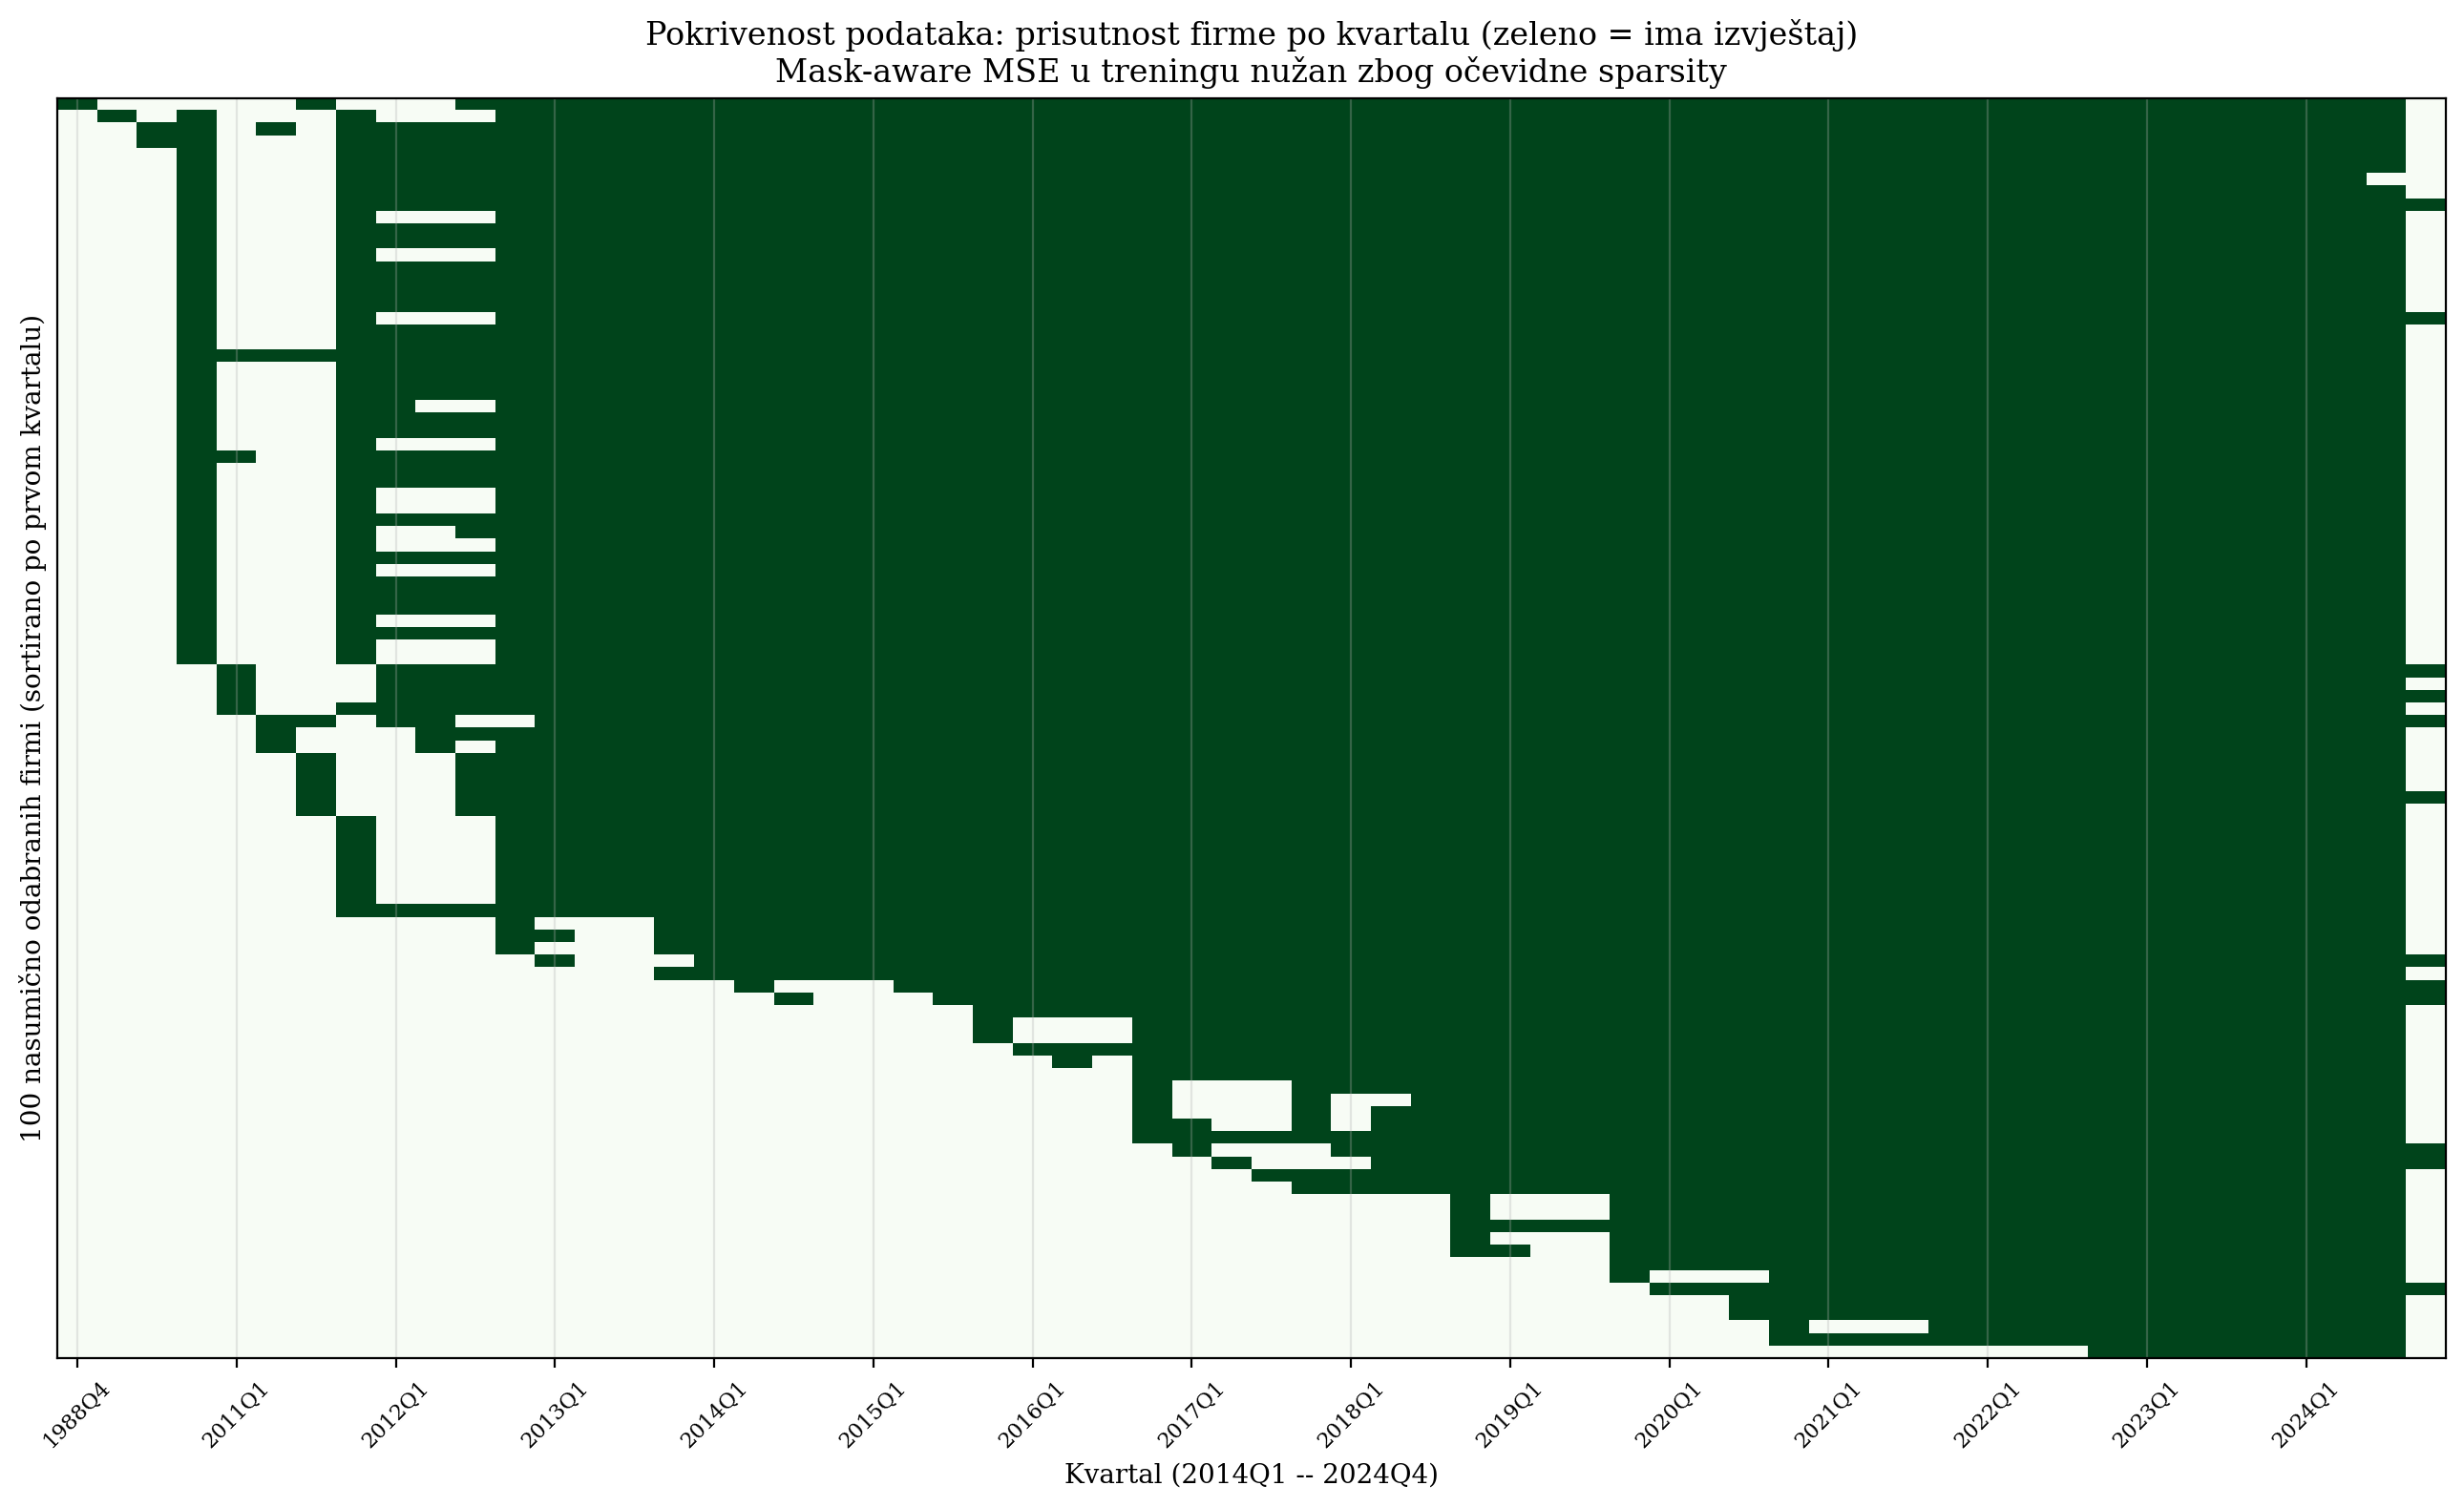
\includegraphics[width=0.95\textwidth]{figures/m_08_coverage_heatmap.png}
 \caption{Pokrivenost podataka: prikaz prisutnosti 100 nasumično odabranih firmi po kvartalu. Zeleno polje označava da firma ima prijavljen izvještaj za taj kvartal. Vidljiva sparsity (firme koje ulaze u/izlaze iz uzorka) opravdava \emph{mask-aware MSE} u treningu.}
 \label{fig:coverage_heatmap}
\end{figure}

\section{Konačne dimenzije panela}

\begin{table}[h]
\centering
\caption{Sažetak izvedenih panela koji ulaze u NN detektore i impact regresor.}
\label{tab:panel_dim}
\begin{tabular}{lrr}
\toprule
Panel & Redovi & Stupci \\
\midrule
\texttt{panel\_quarterly\_raw} & 130.245 & 55 \\
\texttt{panel\_quarterly\_ratios} & 130.245 & 35 \\
\texttt{panel\_quarterly\_ratios\_filled} & 109.956 & 35 \\
\texttt{panel\_annual} & 30.717 & 72 \\
\texttt{sequence\_tensor} (NPZ) & $2.499 \times 44 \times 35$ &, \\
\texttt{daily\_returns} & 1.116.766 & 4 \\
\texttt{restatement\_labels} & 9.351 & 4 \\
\bottomrule
\end{tabular}
\end{table}

\chapter{Modeli za detekciju anomalija}

\section{Princip nenadziranog otkrivanja anomalija rekonstrukcijom}

Sve četiri NN arhitekture koje koristimo dijele isti osnovni princip: model je treniran da \emph{rekonstruira} ulazni vektor iz svojih unutarnjih reprezentacija. Kad model uspješno nauči distribuciju "normalnih" firama, anomalna firma (čije značajke ne pripadaju toj distribuciji) bit će loše rekonstruirana, visoka rekonstrukcijska greška postaje \emph{anomaly score}.

Formalno: za firmu $i$ u periodu $t$ sa značajkama $\mathbf{x}_{i,t} \in \mathbb{R}^F$, model $f_\theta$ producira rekonstrukciju $\hat{\mathbf{x}}_{i,t} = f_\theta(\mathbf{x}_{i,t})$, te se anomaly score definira kao:
\begin{equation}
\text{score}(i, t) = \|\mathbf{x}_{i,t} - \hat{\mathbf{x}}_{i,t}\|_2^2 \cdot \frac{1}{\|\mathbf{m}_{i,t}\|_1}
\label{eq:anomaly_score}
\end{equation}
gdje je $\mathbf{m}_{i,t} \in \{0,1\}^F$ maska koja označava opažene značajke, a normalizacija ekvivalentna je \emph{mask-aware mean squared error}.

\section{Uniformni API}

Svaki detektor implementira identičnu jedinstvenu sheme:
\begin{itemize}
 \item \emph{fit}, nenadzirano treniranje na panelu $X$
 \item \emph{score}, vraća numerički niz anomalijskih ocjena (više $=$ više anomalno)
\end{itemize}
Rezultati svakog detektora pohranjuju se u jedinstvenoj tablici sa shemom (CIK firme, datum perioda, anomalijska ocjena). Ova uniformnost omogućuje da jedinstvena evaluacijska procedura tretira sve detektore identično, što je preduvjet za poštenu usporedbu.

\begin{figure}[h]
 \centering
 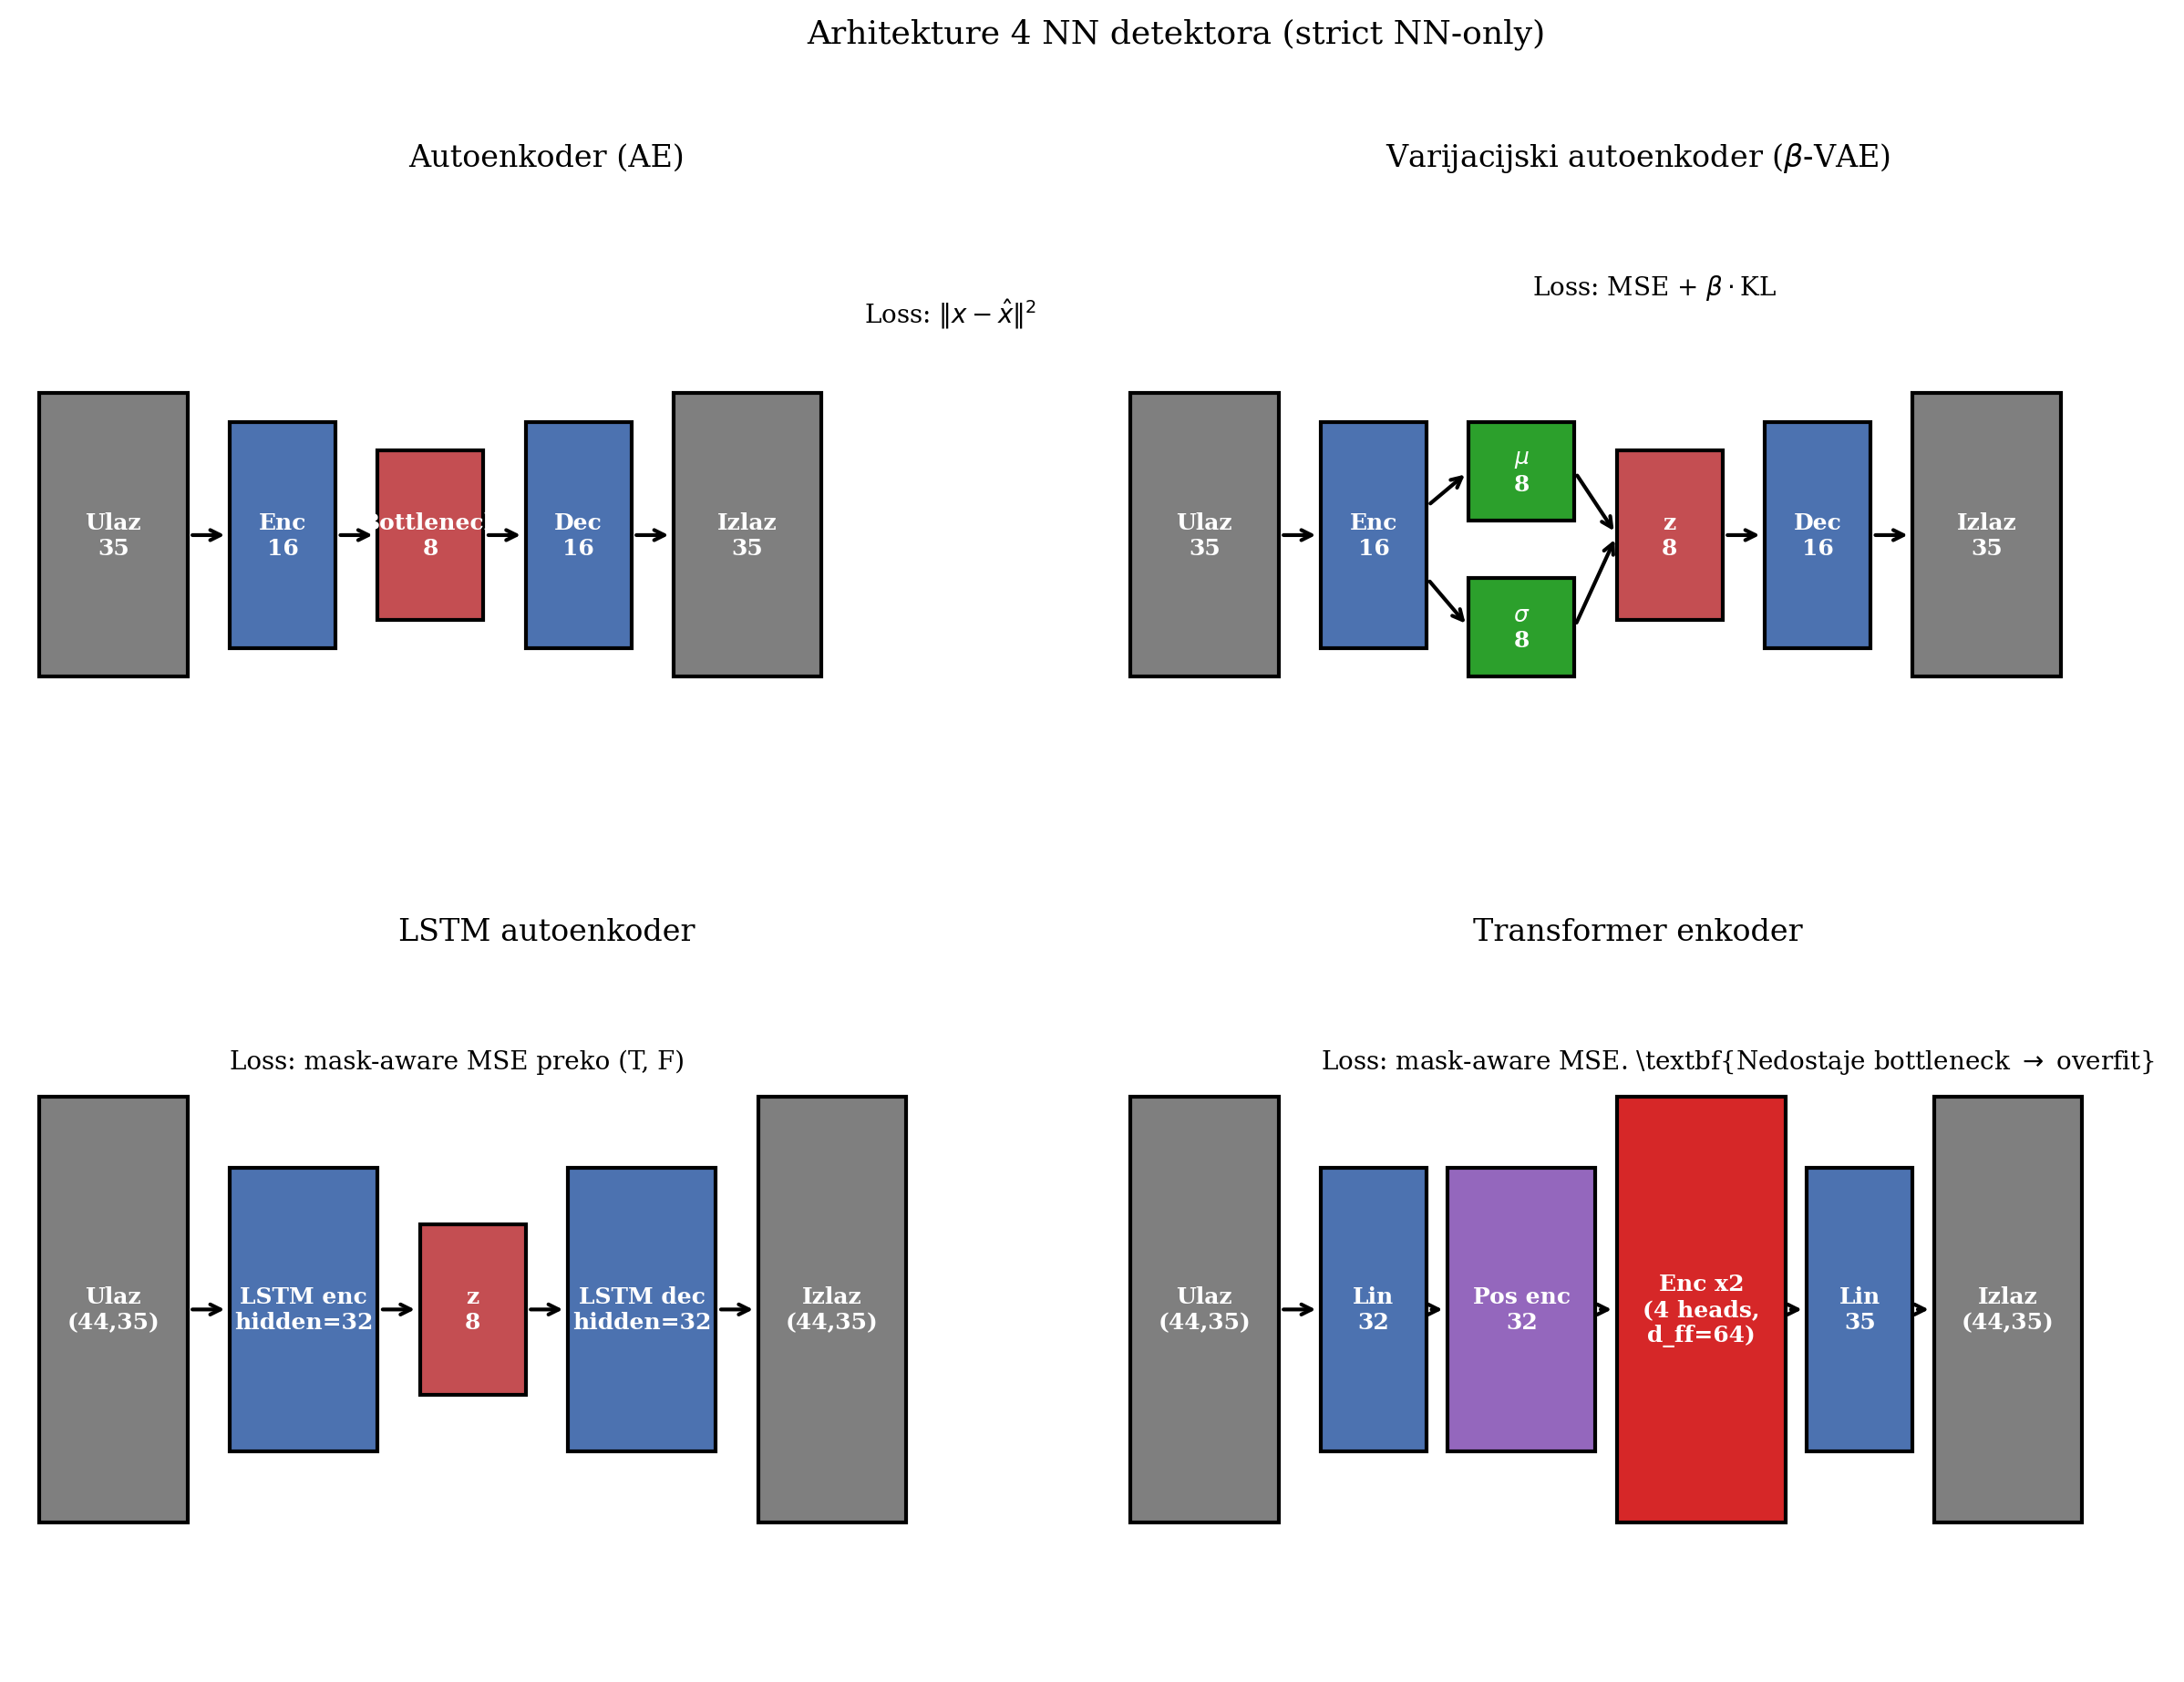
\includegraphics[width=\textwidth]{figures/m_13_arch_schematics.png}
 \caption{Schematski prikaz arhitektura četiri NN detektora. Sve dijele rekonstrukcijski MSE gubitak ali se razlikuju po načinu komprimiranja podataka: AE i VAE statički (bez vremenske dimenzije), LSTM-AE rekurentni, Transformer attention-based. Crveni \emph{bottleneck} sloj u prve tri arhitekture eksplicitno forsira sažimanje; Transformer ga \emph{nema}, što je ključ za njegov overfit footprint u Poglavlju 6.}
 \label{fig:arch_schematics}
\end{figure}

\section{Statički autoenkoder (AE)}

Najjednostavnija od četiri arhitekture, klasični potpuno povezani autoenkoder bez \emph{recurrence} ili \emph{attention}. Tretira svaku firmu-kvartal kao nezavisan ulaz, ignorirajući temporalnu dimenziju.

\textbf{Arhitektura:}
\begin{equation}
\mathbb{R}^{35} \xrightarrow{\text{Linear}+\text{GELU}} \mathbb{R}^{16} \xrightarrow{\text{Linear}+\text{GELU}} \mathbb{R}^{8} \xrightarrow{\text{Linear}+\text{GELU}} \mathbb{R}^{16} \xrightarrow{\text{Linear}} \mathbb{R}^{35}
\label{eq:ae_arch}
\end{equation}

\textbf{Bottleneck} (središnji sloj od 8 jedinica) prisiljava model da nauči kompaktnu reprezentaciju \emph{normalne} firme. Bez bottlenecka, dovoljno bogata mreža bi naučila trivijalnu identitetnu funkciju i ne bi razlikovala normalne od anomalnih firmi.

\textbf{Gubitak:} mask-aware MSE prema jednadžbi \ref{eq:anomaly_score}.

\textbf{Treniranje:} Adam optimizator, $\eta = 10^{-3}$, weight decay $10^{-5}$, 50 epoha, batch size 256. Treniranje je nenadzirano: cijeli panel od 109.956 standardiziranih firma-kvartal vektora služi i kao ulaz i kao željeni izlaz.

\section{Varijacijski autoenkoder (VAE)}

Probabilistička varijanta autoenkodera. Umjesto deterministički mapiranog latentnog vektora $\mathbf{z}$, VAE uči distribuciju $q_\phi(\mathbf{z}|\mathbf{x})$ iz koje se latentna reprezentacija uzorkuje. Ovo regulira latentni prostor da bude geometrijski strukturiran i smanjuje overfitting na pojedinačne ulaze.

\textbf{Arhitektura:} encoder mapira $\mathbf{x} \in \mathbb{R}^{35}$ u parametre $(\boldsymbol{\mu}, \log\boldsymbol{\sigma}^2) \in \mathbb{R}^{8} \times \mathbb{R}^{8}$ Gaussove distribucije u latentnom prostoru. Pri treniranju, $\mathbf{z}$ se uzorkuje pomoću \emph{reparameterization trika} $\mathbf{z} = \boldsymbol{\mu} + \boldsymbol{\sigma} \odot \boldsymbol{\epsilon}$, $\boldsymbol{\epsilon} \sim \mathcal{N}(0, I)$. Decoder rekonstruira ulaz iz $\mathbf{z}$.

\textbf{Gubitak} (negativan ELBO) ima dvije komponente:
\begin{equation}
\mathcal{L}_{\text{VAE}} = \underbrace{\|\mathbf{x} - \hat{\mathbf{x}}\|_2^2}_{\text{rekonstrukcija}} + \beta \cdot \underbrace{\mathrm{KL}\left( q_\phi(\mathbf{z}|\mathbf{x}) \,\Vert\, \mathcal{N}(0, I) \right)}_{\text{regularizacija}}
\end{equation}

Koristimo $\beta = 0{,}5$ (umjereno potisnut KL term) da model ne kolabira u trivijalan posterior. \emph{Anomaly score} = MSE rekonstrukcije (kompatibilno s ostalim arhitekturama; alternativna formulacija $-\log p(\mathbf{x})$ daje slične ali ne identične rangove).

\textbf{Treniranje:} isti optimizator i hiperparametri kao AE.

\section{LSTM autoenkoder}

Prva sekvencijalna arhitektura. Tretira svaku firmu kao sekvencu od 44 kvartalnih vektora i koristi LSTM \citep{hochreiter1997} za enkodiranje temporalne dinamike.

\textbf{Arhitektura:}
\begin{itemize}
 \item \textbf{Encoder LSTM:} hidden dimenzija 32, jedan sloj. Procesira $(T=44, F=35)$ sekvencu, vraća konačno stanje $\mathbf{h}_T \in \mathbb{R}^{32}$.
 \item \textbf{Latent layer:} linearna projekcija $\mathbf{h}_T \to \mathbf{z} \in \mathbb{R}^{8}$ (bottleneck).
 \item \textbf{Decoder LSTM:} prima ponovljenu $\mathbf{z}$ na svakom vremenskom koraku $(T=44, 32)$ i rekonstruira sekvencu.
 \item \textbf{Output projekcija:} linearna $\mathbb{R}^{32} \to \mathbb{R}^{35}$ na svakom koraku.
\end{itemize}

\textbf{Gubitak:} mask-aware MSE po svim opaženim pozicijama (firma $\times$ kvartal $\times$ značajka).

\textbf{Motivacija:} hipoteza je da firmin temporalni obrazac (npr.\ glatka rast prihoda kroz godine vs.\ iznenadni skokovi) sadrži forenzički signal koji statički AE ne može uhvatiti. Anomalije koje statički AE propušta, jer su \emph{trajektorijalno} neobične iako svaka pojedinačna točka izgleda normalno, LSTM-AE bi trebao detektirati kroz lošu rekonstrukciju sekvence.

\textbf{Treniranje:} Adam, $\eta = 10^{-3}$, weight decay $10^{-5}$, 50 epoha, batch size 64 (manji nego AE jer su sekvence memorijski teže).

\section{Transformer enkoder}

Druga sekvencijalna arhitektura, koristi \emph{self-attention} mehanizam \citep{vaswani2017} umjesto rekurencije. Implementacija je inspirirana PatchTST-om \citep{nie2023} za vremenske serije, ali pojednostavljena.

\textbf{Arhitektura:}
\begin{itemize}
 \item \textbf{Input projekcija:} linearna $\mathbb{R}^{35} \to \mathbb{R}^{32}$ na svakom vremenskom koraku (\emph{token embedding}).
 \item \textbf{Sinusoidalni pozicijski encoding} $(T=44, d_{\text{model}}=32)$ dodaje informaciju o vremenskoj poziciji.
 \item \textbf{Transformer enkoder:} 2 sloja s 4 \emph{attention head}-a po sloju, GELU aktivacijom, $d_{\text{ff}}=64$ za \emph{feed-forward} mrežu.
 \item \textbf{Output projekcija:} linearna $\mathbb{R}^{32} \to \mathbb{R}^{35}$ na svakom koraku.
\end{itemize}

\textbf{Self-attention} omogućuje da svaki kvartal direktno "vidi" sve ostale kvartale firme pri rekonstrukciji, za razliku od LSTM-a koji informaciju propušta kroz skrivena stanja korak po korak. Teoretski je to prednost za firme s dugoročnim obrascima (npr.\ ciklični uzorak prihoda kroz 5 godina), ali zahtijeva više podataka i sklonija je \emph{overfitting}-u.

\textbf{Gubitak:} mask-aware MSE.

\textbf{Treniranje:} isti hiperparametri kao LSTM. \textbf{Ograničenje}: u našem eksperimentu Transformer training gubitak kolapsira na $0{,}026$ (značajno niže od ostalih modela), što je \emph{fingerprint overfittinga}. Ovo se manifestira u sekciji rezultata 6.1 kao niži supervised ROC-AUC od AE/VAE/LSTM. Diskutirano u sekciji 7.3 kao metodološko opažanje: arhitekture bez eksplicitnog bottlenecka mogu naučiti trivijalna identitetna mapiranja, eliminirajući anomaly signal.

\section{Sažetak parametara modela}

\begin{table}[h]
\centering
\caption{Hiperparametri za četiri NN detektora. Sve modele treniramo 50 epoha s Adam optimizerom ($\eta=10^{-3}$, weight decay $10^{-5}$).}
\label{tab:model_params}
\begin{tabular}{lcccc}
\toprule
 & \textbf{AE} & \textbf{VAE} & \textbf{LSTM-AE} & \textbf{Transformer} \\
\midrule
Tip & statički & statički + KL & rekurentni & self-attention \\
Ulaz & vektor $35$ & vektor $35$ & sekvenca $(44,35)$ & sekvenca $(44,35)$ \\
Hidden / $d_{\text{model}}$ & 16, 8 & 16, 8 + $\sigma$ & 32 & 32 \\
Slojeva enkoder/dekoder & 2/2 & 2/2 & 1/1 & 2 (enkoder) \\
Bottleneck dim & 8 & 8 & 8 &, (implicitan) \\
Broj parametara & $\approx 1{,}5$ k & $\approx 1{,}7$ k & $\approx 9$ k & $\approx 17$ k \\
Batch size & 256 & 256 & 64 & 64 \\
\bottomrule
\end{tabular}
\end{table}

\section{Treniranje na cijelom uzorku (\emph{transductive setting})}

Svi modeli treniraju se na cijelom panelu (svih 109.956 firma-kvartala, sva poduzeća, sve godine). Ne razdvajamo trening i test skup za samu detekciju jer:
\begin{enumerate}
 \item Treniranje je strogo nenadzirano, nema oznaka koje bi se mogle \emph{procuriti}.
 \item Cilj nije generalizacija na nove firme nego identifikacija anomalnih firmi unutar danog skupa, to je \emph{transductive} a ne \emph{inductive} problem.
 \item Vremenska podjela se primjenjuje na razini \emph{evaluacije} (sekcija 6.4: train na 2014--2021, test na 2022--2024 za supervised eval), ne na razini detektora.
\end{enumerate}

Ovo je standardna praksa u literaturi nenadzirane detekcije anomalija \citep{aggarwal2017} i razlikuje se od supervised klasifikacije gdje su trening i test obvezno odvojeni.

\section{Reproducibilnost}

Svi modeli koriste fiksne nasumične sjemenke (\emph{seeds}):
\begin{itemize}
 \item fiksna PyTorch sjemenka, inicijalizacija težina, \emph{DataLoader} shuffle
 \item fiksna NumPy sjemenka, ostale numpy operacije
\end{itemize}

Robusnost rezultata na izbor sjemenke evaluirana je u sekciji 6.6 kroz 5-seed replikaciju \emph{impact regresora} (sjemenke $\{42, 7, 123, 2024, 9999\}$).

\begin{figure}[h]
 \centering
 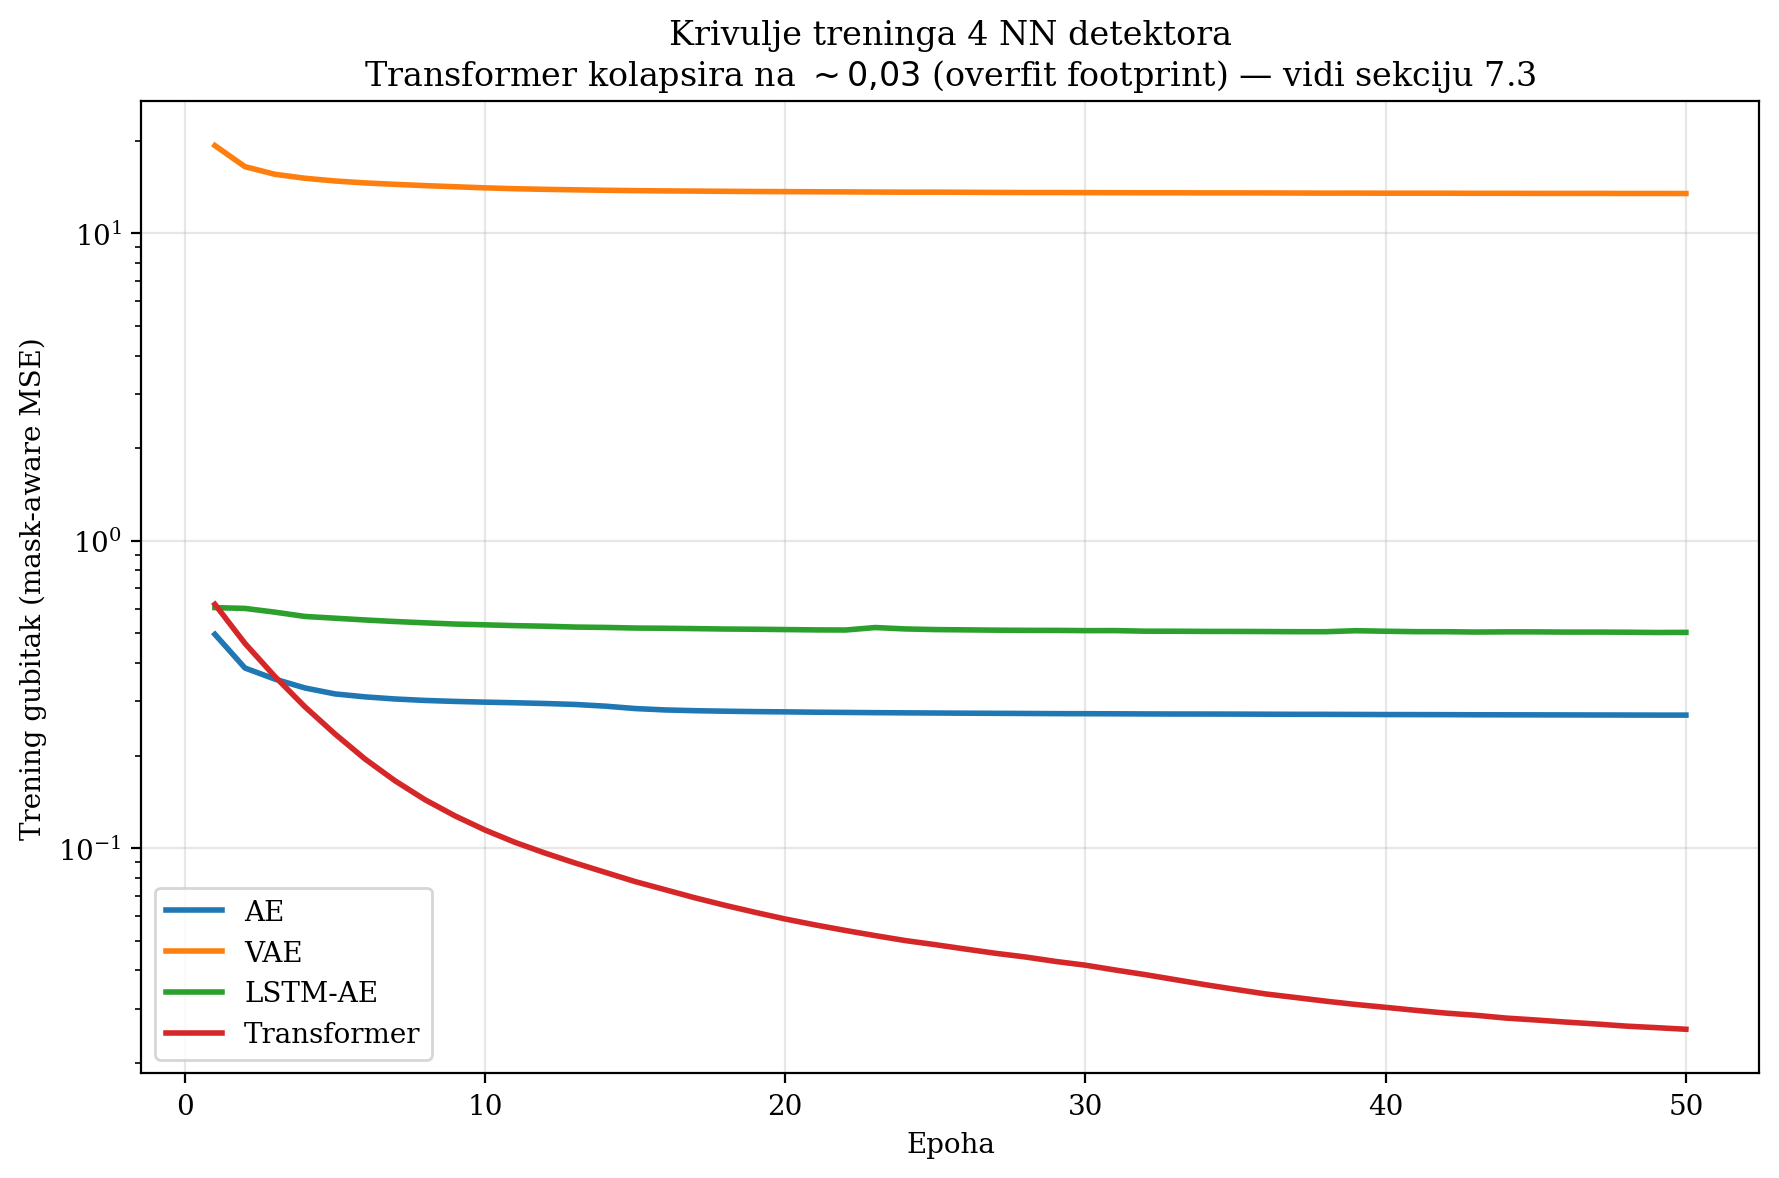
\includegraphics[width=0.9\textwidth]{figures/m_04_training_loss.png}
 \caption{Krivulje trening gubitka kroz 50 epoha za 4 NN detektora (log skala). AE, VAE i LSTM-AE konvergiraju na nivo $\sim 0{,}1$, što reflektira nesavršenost rekonstrukcije nad heterogenim financijskim podacima. Transformer enkoder, međutim, kolapsira na gubitak $\sim 0{,}03$, \emph{otisak overfittinga} koji proizlazi iz nedostatka eksplicitnog bottlenecka u arhitekturi (vidi sekciju 7.3).}
 \label{fig:training_loss}
\end{figure}

\chapter{Predikcija utjecaja: NN regresor}

\section{Motivacija: zašto NN umjesto OLS-a}

Drugi dio teze, "utjecaj identificiranih anomalija na poslovanje kompanije", klasično bi se rješavao linearnom regresijom (OLS) ili event-study analizom kumulativnog abnormalnog prinosa. Međutim, naslov teme eksplicitno postavlja \emph{neural networks} kao metodu istraživanja. Stoga koristimo \emph{strogo NN-only} pristup: anomaly score iz NN detektora ulazi u NN regresor (MLP) koji predviđa tržišni ishod.

Sekundarna metodološka prednost: NN MLP može uhvatiti \emph{nelinearne interakcije} između anomaly score-a i kontrolnih varijabli (npr.\ "visok anomaly score $+$ visok rast firme $\to$ posebno visoka volatilnost"). Klasični OLS bi takvu interakciju propustio bez eksplicitnih interakcijskih termina.

Klasične metode (event study, propensity matching, OLS) razrađene su kao reference izvan glavnog narativa, ali nisu u primarnom narativu rada.

\section{Specifikacija MLP regresora}

\textbf{Arhitektura:}
\begin{equation}
\mathbf{x}_{\text{kombinirano}} \xrightarrow{\text{Linear}+\text{GELU}+\text{Dropout}_{0{,}2}} \mathbb{R}^{32} \xrightarrow{\text{idem}} \mathbb{R}^{32} \xrightarrow{\text{idem}} \mathbb{R}^{32} \xrightarrow{\text{Linear}} \mathbb{R}^{1}
\end{equation}

3 skrivena sloja od po 32 jedinice, GELU aktivacija \citep{hendrycks2016}, dropout od $0{,}2$ između slojeva, MSE gubitak.

\textbf{Ulazni vektor} $\mathbf{x}_{\text{kombinirano}}$:
\begin{enumerate}
 \item \textbf{score\_t} (anomaly score iz NN detektora u godini $t$)
 \item \textbf{log\_assets} (logaritam imovine u godini $t$, kontrola veličine firme)
 \item \textbf{revenue\_growth} (rast prihoda $t-1 \to t$, winsorizirano $[-2, 2]$)
 \item \textbf{asset\_growth} (rast imovine $t-1 \to t$, winsorizirano $[-2, 2]$)
 \item \textbf{sektorske dummy varijable} (SIC 2-digit, drop-first encoded $\to$ 56 dummy stupaca)
\end{enumerate}

Napomena o sektorskoj granularnosti: za cross-sektorsku $z$-skor standardizaciju (Poglavlje 3.4) koristimo grublju SIC 1-digit razinu (10 grupa) jer je za stabilne procjene $\mu$, $\sigma$ potreban dovoljan uzorak. Ovdje, za regresor kontrola, koristimo finiju SIC 2-digit razinu (57 sektora) jer MLP može iskoristiti veću granularnost bez problema malog uzorka, regresor uči na cijelom panelu, ne po grupi.

Konkretna ulazna dimenzija: $4 + 56 = 60$.

\textbf{Treniranje:} Adam, $\eta = 10^{-3}$, weight decay $10^{-5}$, 80 epoha (više nego za detektore jer regresijska zadaća zahtijeva preciznije fitanje), batch size 256.

\section{Ishodi koji se predviđaju}

Četiri tržišna ishoda za godinu $t+1$ (jedna godina unaprijed od detekcije anomalije):

\begin{enumerate}
 \item \textbf{annual\_return\_market}: godišnji prinos dionice u godini $t+1$, izračunat kao $\sum_{d \in t+1} \log(P_d / P_{d-1})$.
 \item \textbf{volatility\_market}: godišnja volatilnost, $\sigma$ dnevnih log-prinosa $\times \sqrt{252}$.
 \item \textbf{max\_drawdown\_market}: maksimalan \emph{peak-to-trough} pad cijene u godini $t+1$. Negativan broj (npr.\ $-0{,}40$ znači maksimalan pad od $40\,\%$ od bilo kojeg vrhunca).
 \item \textbf{volume\_growth\_market}: promjena prosječnog dnevnog volumena trgovanja, log-diff (godina $t+1$ vs godina $t$).
\end{enumerate}

Svaki ishod tretira se kao zasebna regresijska zadaća. Trenira se 4 detektora $\times$ 4 ishoda $=$ 16 modela.

\section{Kritična metodološka stavka: kontrola za rast firme}

\emph{Problem confounding-a.} Bez kontrole za rast firme, NN detektor koji označava visoko-rastuće firme kao "anomalne" producirao bi visoki $\Delta R^2$ za volatilnost, ne zato što je anomalija prediktivna, nego zato što su visoko-rastuće firme \emph{mehanički} volatilnije (početne firme, post-IPO firme, itd.). Anomaly score bi tako bio samo \emph{proxy} za rast.

\emph{Dijagnostika u podacima.} Tijekom analize utvrđeno je da su firme s najvišim NN anomaly score-om sustavno bile high-growth firme tehnološkog sektora (npr.\ NVDA, koja je u 2023.\ godini rasla $\sim 200\,\%$ i bila top-anomalna po više detektora). Bez kontrole, "DL detektor predviđa $+4{,}8$ p.b.\ volatilnosti" bila bi nepoštena tvrdnja: značajan udio tog signala je rast u prerušavanju.

\emph{Rješenje, partial-out.} Dodaju se revenue\_growth i asset\_growth kao eksplicitne kontrole. NN regresor sada mora pronaći varijaciju u ishodu koja \emph{nije objašnjena} rastom. Ono što ostaje pripisivo anomaly score-u je \emph{rezidualan signal}, pravi forenzički doprinos.

\emph{Empirijska kvantifikacija.} Sekcija 6.7 (tablica \ref{tab:pre_post_growth}) prikazuje smanjenja od 40\,--\,80\,\% u $\Delta R^2$ nakon dodavanja growth controls, ovisno o detektoru i ishodu. Konkretno za LSTM-AE volatilnost: single-seed pre-R1-fix pristup daje $+0{,}048 \to +0{,}008$ ($-82\,\%$); single-seed post-R1-fix daje $+0{,}048 \to +0{,}019$ ($-60\,\%$); 5-seed mean post-fix daje $+0{,}029 \pm 0{,}008$. Sve tri verzije pokazuju materijalnu redukciju zbog growth confound-a. Ovo je \textbf{glavna metodološka kontribucija rada}, ova kontrola je rijetko primijenjena u sličnoj DL literaturi za forenzičko računovodstvo.

\section{Temporalna train/test podjela}

Klasični OLS s cluster-robusnim standardnim greškama (na razini firme) je standard u financijskoj literaturi. Međutim, naš NN regresor lako overfita ako se evaluira na istim godinama na kojima trenira. Stoga koristimo \textbf{temporalnu podjelu}:

\begin{itemize}
 \item \textbf{Trening:} firma-godine s $t < 2022$ ($n_{\text{train}} \approx 14.237$ nakon NaN-drop-ova)
 \item \textbf{Test:} firma-godine s $t \geq 2022$ ($n_{\text{test}} \approx 4.291$)
\end{itemize}

Ovo je strogi \emph{hold-out}, model nikad ne vidi 2022.\,--\,2024.\ podatke tijekom treninga. Out-of-sample $R^2$ na testu je stoga \emph{nepristrana} mjera generalizacijske sposobnosti, otporna na overfitting.

\textbf{Standardizacija ulaza.} Sve ulazne varijable ($\mathbf{x}$) i izlazni ishod ($y$) standardiziraju se koristeći \emph{samo trening-set statistike} $(\mu, \sigma)$, koje se zatim primijenjuju i na test-set. Time se sprečava curenje informacija iz testa u trening.

\section{Glavne metrike}

\subsection{Out-of-sample delta-$R^2$}

Glavna metrika je:
\begin{equation}
\Delta R^2 = R^2_{\text{full}} - R^2_{\text{baseline}}
\end{equation}
gdje $R^2_{\text{full}}$ je $R^2$ na test-setu MLP regresora s anomaly\_score \emph{kao ulazom}, a $R^2_{\text{baseline}}$ je $R^2$ identičnog MLP regresora s istim kontrolama \emph{ali bez anomaly\_score-a}. $\Delta R^2$ tako mjeri \emph{inkrementalnu} prediktivnu vrijednost anomalije iznad onoga što kontrole već daju.

Pozitivni $\Delta R^2$ znači da anomaly score donosi novu informaciju izvan rasta, veličine i sektora.

\subsection{Permutation importance}

Komplementarna metrika koja koristi \emph{istu} obučenu mrežu kao za $R^2_{\text{full}}$:
\begin{equation}
\text{perm\_importance} = \frac{1}{N_{\text{rep}}} \sum_{r=1}^{N_{\text{rep}}} \left( R^2_{\text{unshuffled}} - R^2_{\text{shuffled-r}} \right)
\end{equation}
gdje shuffle se primjenjuje samo na stupcu anomaly\_score u test-setu. $N_{\text{rep}} = 5$ ponavljanja. Pad $R^2$ kad shuffle uništi informaciju u anomaly score-u je mjera njegove važnosti za već obučeni model.

Permutation importance često je \emph{viša} od $\Delta R^2$ jer hvata signal koji se gubi pri usporedbi s baseline modelom (baseline može preuzeti dio signala kroz korelirane kontrole; permutation izolira čisti score doprinos).

\subsection{Robustnost: 5-seed replikacija}

Kako bi se osiguralo da rezultati nisu artefakt jedne slučajne sjemenke, cijeli pipeline ponavlja se 5 puta s sjemenkama $\{42, 7, 123, 2024, 9999\}$. Za svaki par (detektor, ishod) izvještava se \emph{mean} $\pm$ \emph{std} preko 5 sjemenki, te broj sjemenki s pozitivnim $\Delta R^2$ ($n_{\text{pos}}/5$).

Rezultat se smatra \emph{robusnim} ako je $n_{\text{pos}} \geq 4/5$ i $|\text{mean}| > \text{std}$.

\chapter{Rezultati}

\section{Detekcijske performanse (RQ1)}

Tablica \ref{tab:detection_results} prikazuje supervised evaluaciju četiri NN detektora protiv \emph{restatement} oznaka iz SEC EDGAR-a (10-K/A i 10-Q/A obrazaca), s bootstrap 95\,\% intervalom povjerenja preko 1.000 resampleova. Iako trening svih detektora ostaje strogo nenadziran, ova evaluacija pruža objektivnu mjeru kvalitete detekcije naspram poznatih slučajeva ispravljenog izvještaja.

\begin{table}[h]
\centering
\caption{Supervised evaluacija NN detektora protiv \emph{restatement} oznaka. Univerzum: Russell 3000, 30.591 firma-godina, bazna stopa restatementa 2,37\,\%.}
\label{tab:detection_results}
\begin{tabular}{lcccccc}
\toprule
Detektor & ROC-AUC & PR-AUC & prec@10 & prec@100 & lift@100 \\
\midrule
AE & 0,650 & 0,052 & 0,10 & 0,16 & $6{,}76\times$ \\
VAE & 0,650 & 0,052 & 0,10 & 0,15 & $6{,}34\times$ \\
LSTM-AE & 0,637 & 0,052 & 0,10 & 0,16 & $6{,}76\times$ \\
Transformer & 0,616 & 0,045 & 0,10 & 0,11 & $4{,}65\times$ \\
\midrule
Bazna stopa & 0,500 & 0,024 &, & 0,024 & $1{,}00\times$ \\
\bottomrule
\end{tabular}
\end{table}

\textbf{Ključno opažanje}: tri od četiri detektora (AE, VAE, LSTM-AE) konvergiraju na ROC-AUC približno 0,64\,--\,0,65 s 95\,\% bootstrap intervalima koji se međusobno preklapaju. \textbf{Konvergencija arhitektura} je empirijski potvrđena: razlike između statičke (AE), probabilističke (VAE) i rekurentne (LSTM) arhitekture nisu statistički značajne na razini AUC. Transformer encoder ostaje za bod-dvije iza, vjerojatno zbog overfittinga (vidi sekciju 7.3).

\textbf{Lift@100} od $6{,}76\times$ znači da pretraživanje top 100 firmi po anomaly score-u identificira 16\,\% restated firmi naspram bazne stope od 2,4\,\%, iako daleko od savršenosti, značajno bolje od slučajnog pretraživanja.

\begin{figure}[h]
 \centering
 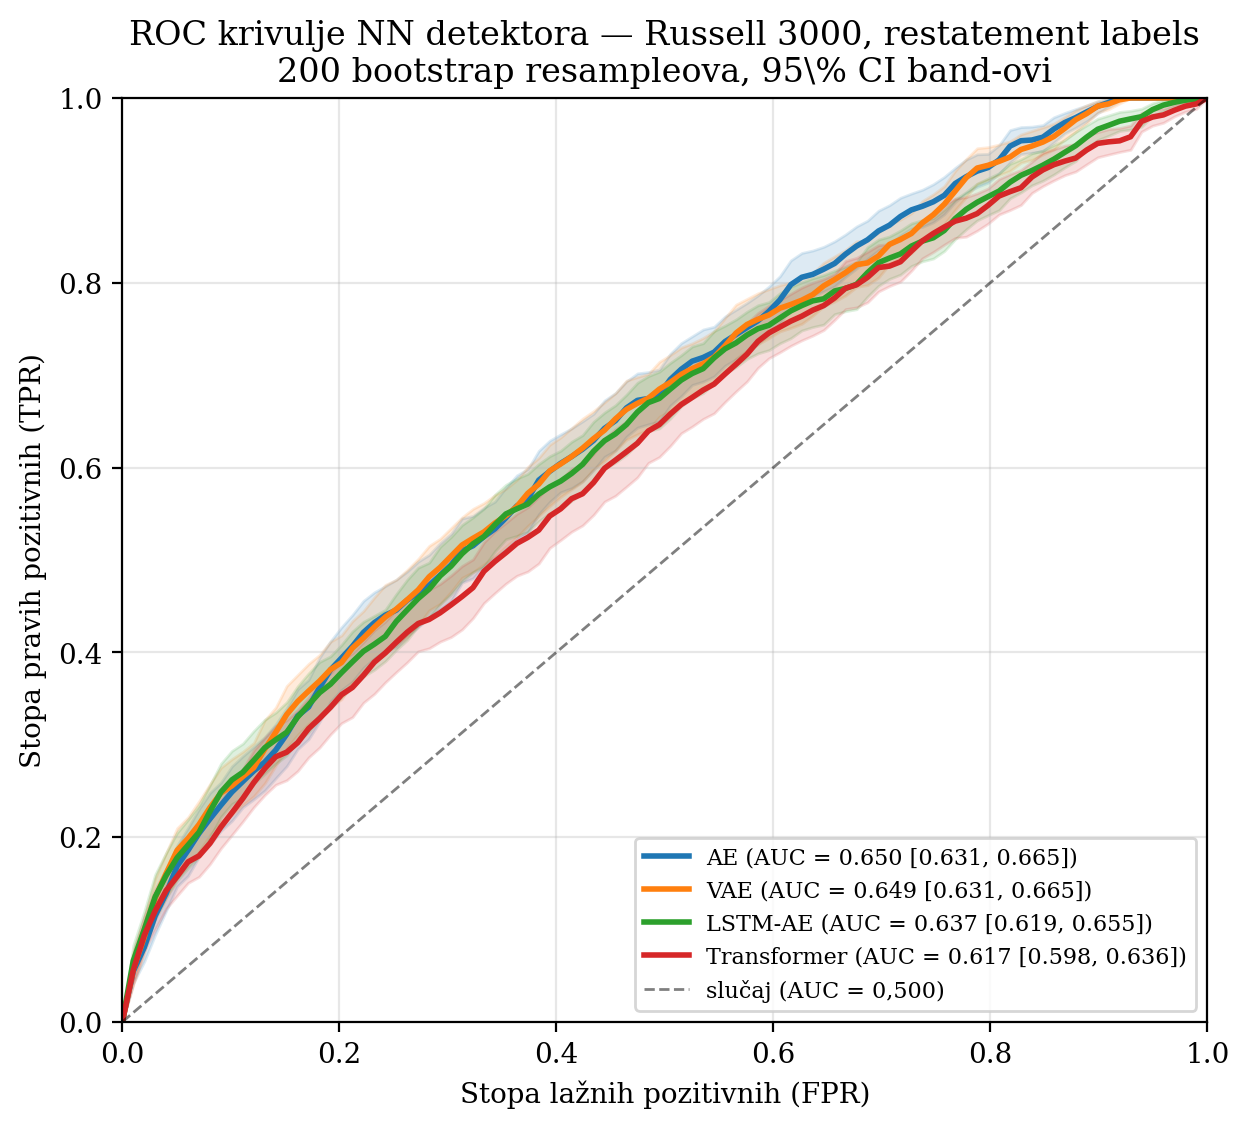
\includegraphics[width=0.85\textwidth]{figures/m_01_roc_curves.png}
 \caption{ROC krivulje 4 NN detektora s 95\,\% bootstrap CI band-ovima (200 resampleova). Krivulje praktički preklapaju, vizualna demonstracija \emph{konvergencije arhitektura}. Transformer (crveno) ima najnižu AUC, dosljedno s overfittingom.}
 \label{fig:roc_curves}
\end{figure}

\begin{figure}[h]
 \centering
 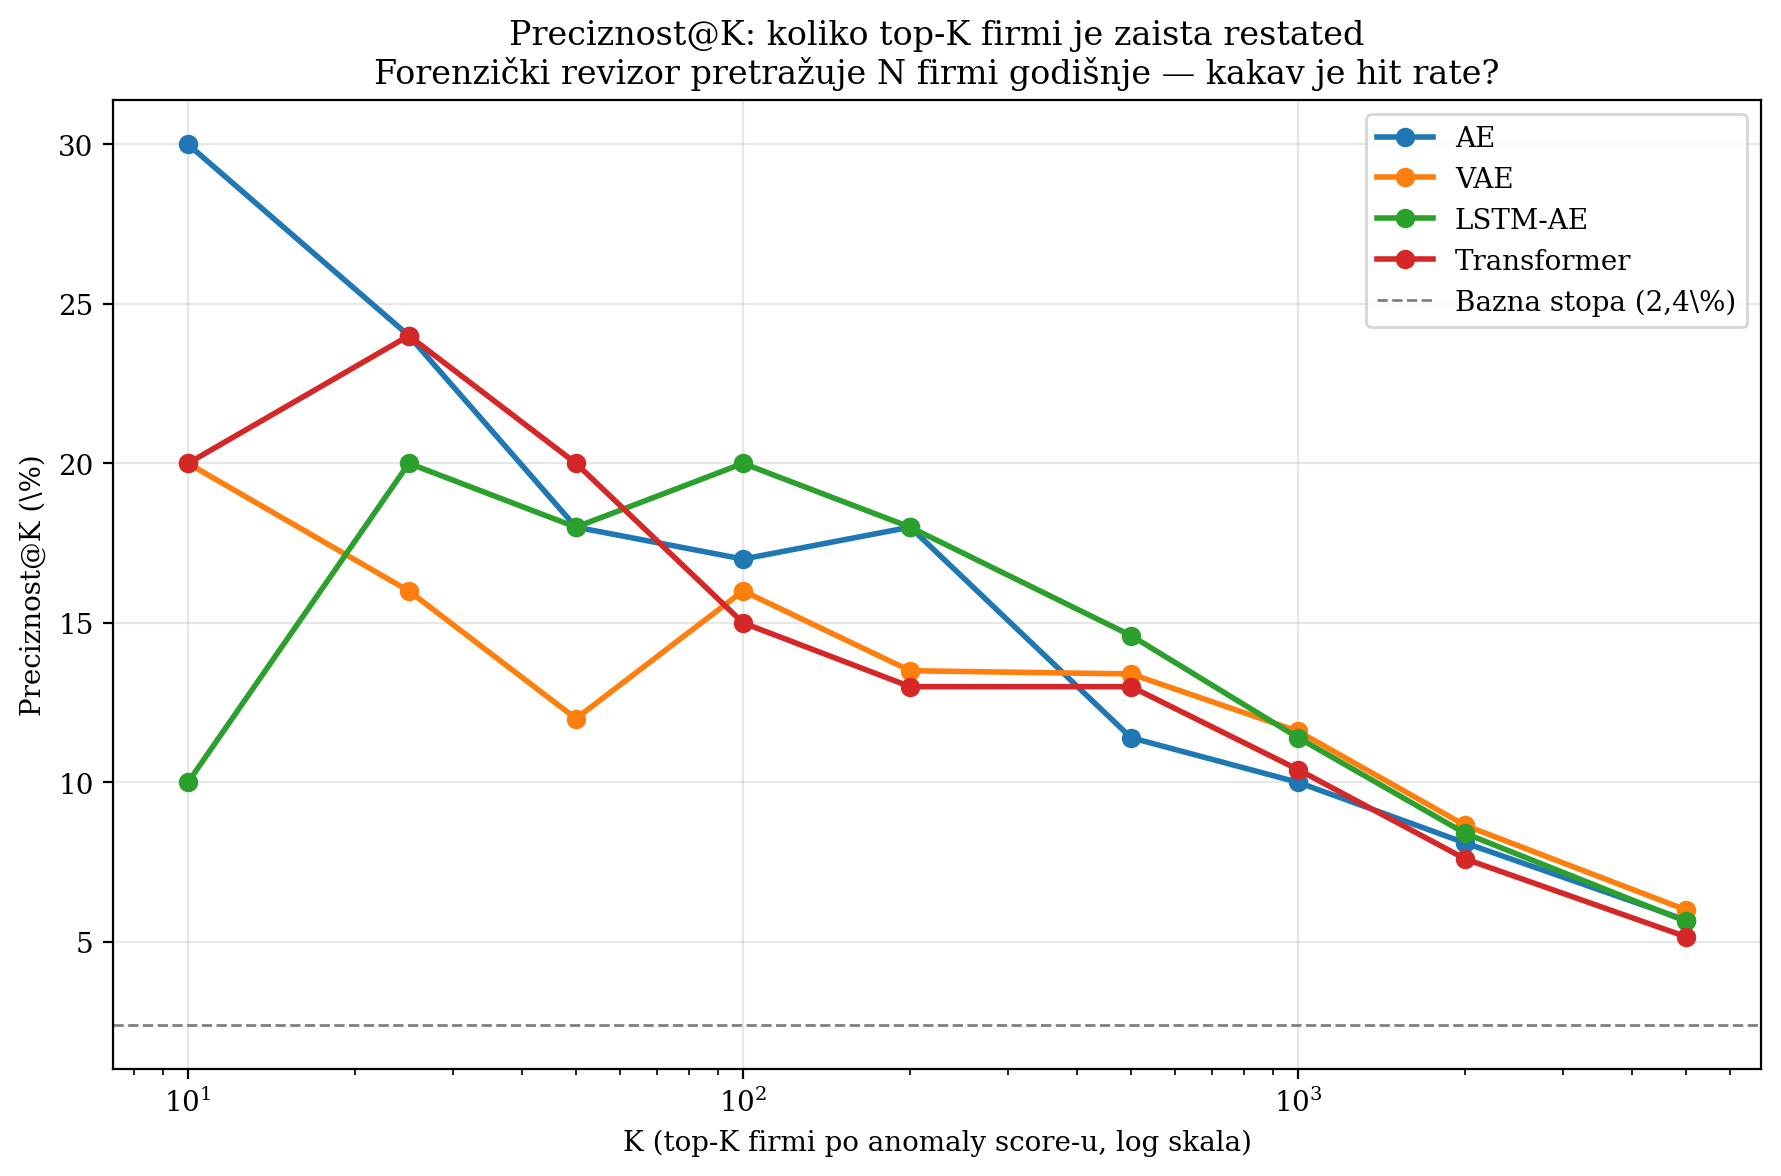
\includegraphics[width=0.85\textwidth]{figures/m_10_precision_at_k.png}
 \caption{Preciznost@K krivulja (log K) za 4 NN detektora protiv \emph{restatement} oznaka. Forenzički revizor koji pretražuje top-100 ima približno 16\,\% hit rate (AE/VAE/LSTM-AE) naspram bazne stope 2,4\,\%.}
 \label{fig:precision_at_k}
\end{figure}

\begin{figure}[h]
 \centering
 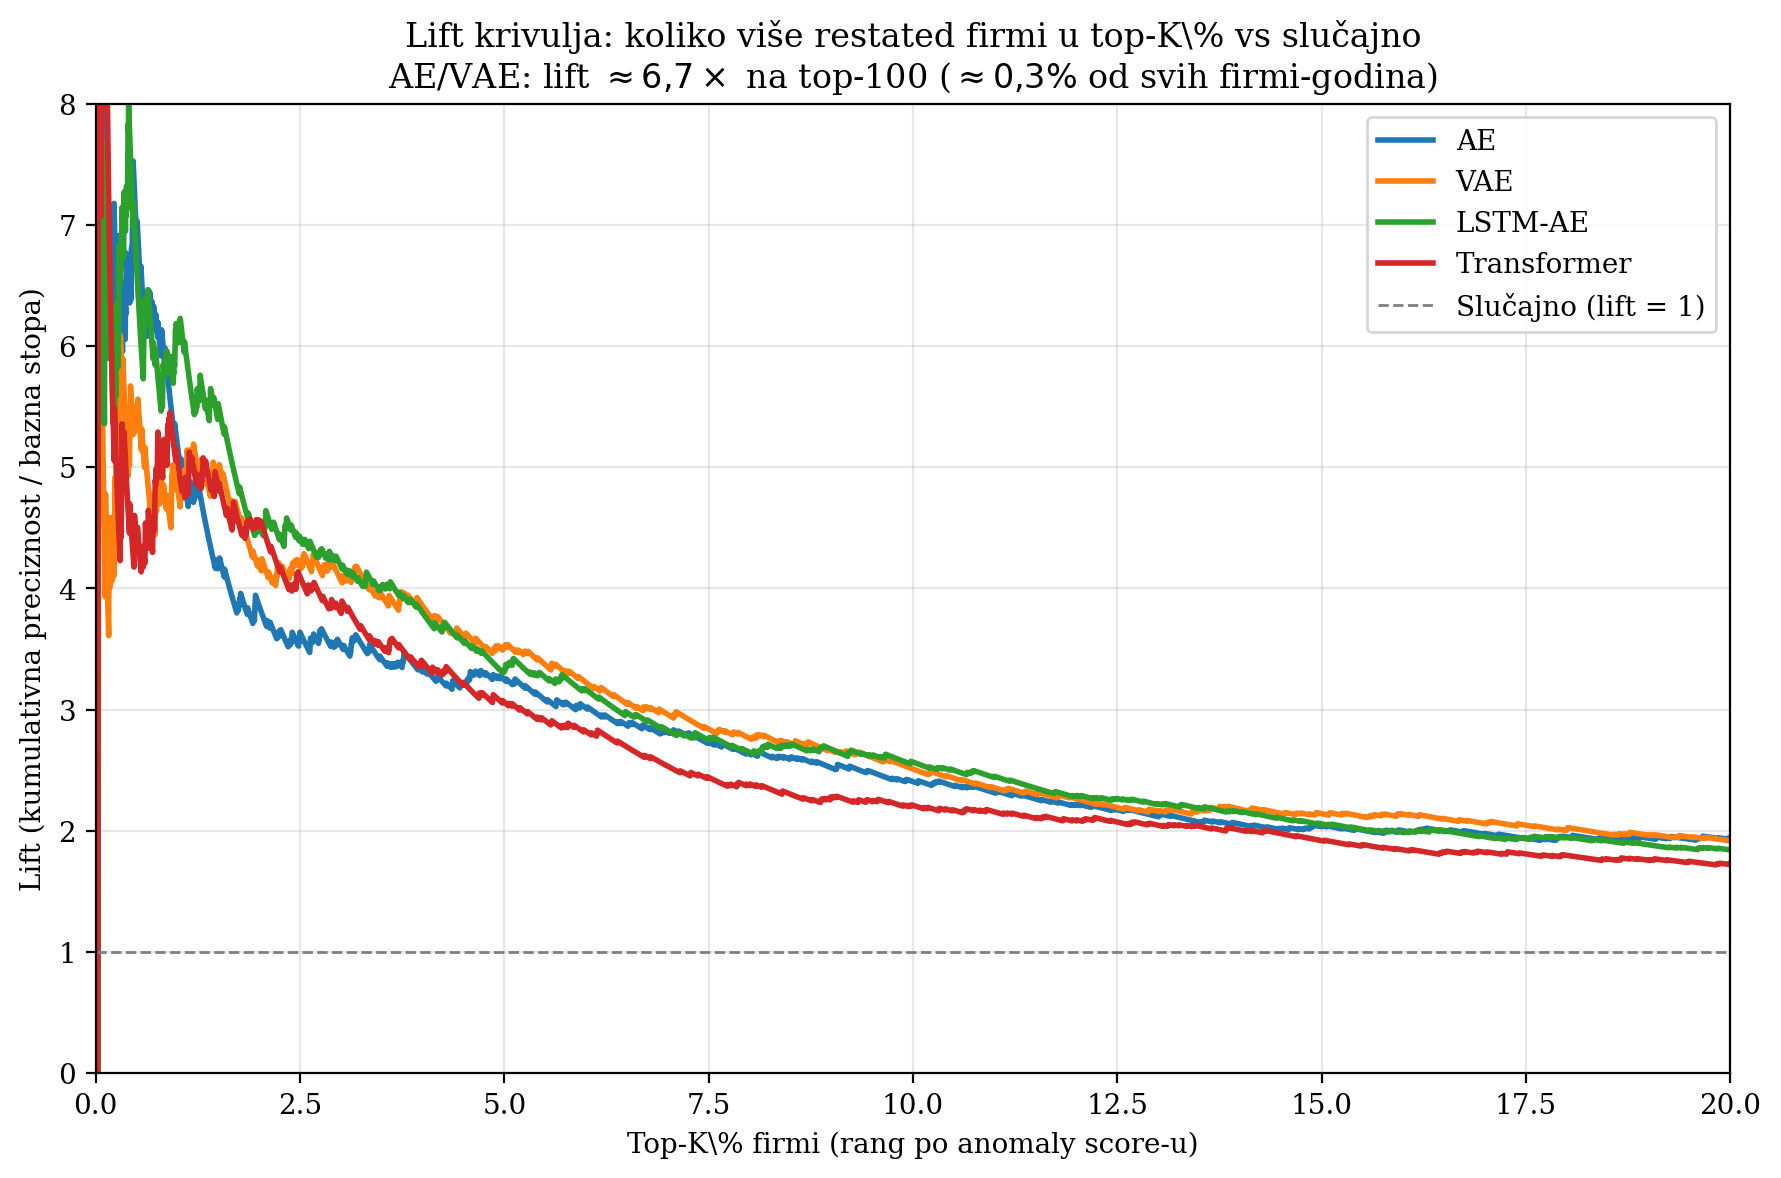
\includegraphics[width=0.85\textwidth]{figures/m_16_lift_curve.png}
 \caption{Lift krivulja: omjer kumulativne preciznosti i bazne stope, kao funkcija postotka top-K firmi. Na top-1\,\% (otprilike top-300 firma-godina) AE i VAE postižu lift $\approx 6\times$. Lift opada s većim K-om, što se očekuje za bilo koji detektor.}
 \label{fig:lift_curve}
\end{figure}

\begin{figure}[h]
 \centering
 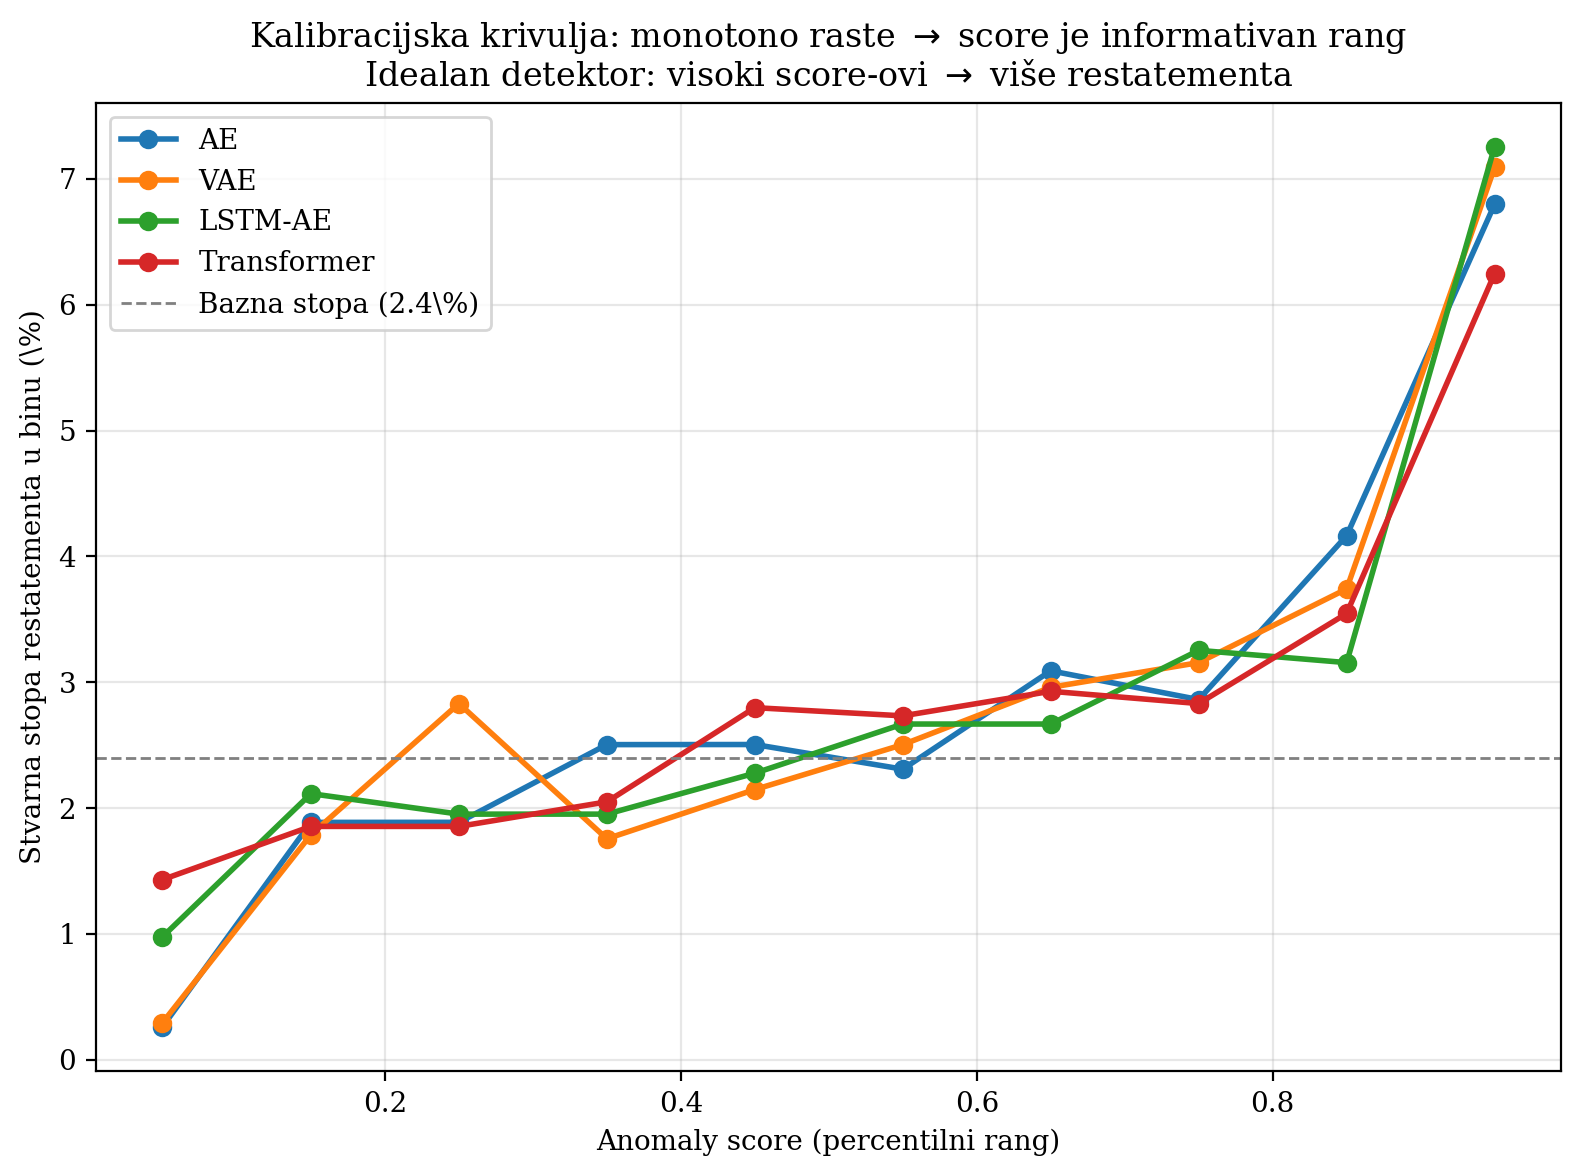
\includegraphics[width=0.85\textwidth]{figures/m_15_calibration.png}
 \caption{Kalibracijska krivulja: stvarna stopa restatementa u bin-u (Y) vs.\ percentilni rang anomaly score-a (X). Monotonu rast kod sva 4 detektora potvrđuje da su score-ovi informativan rang. AE i VAE su najstrmiji u gornjim percentilima.}
 \label{fig:calibration}
\end{figure}

\begin{figure}[h]
 \centering
 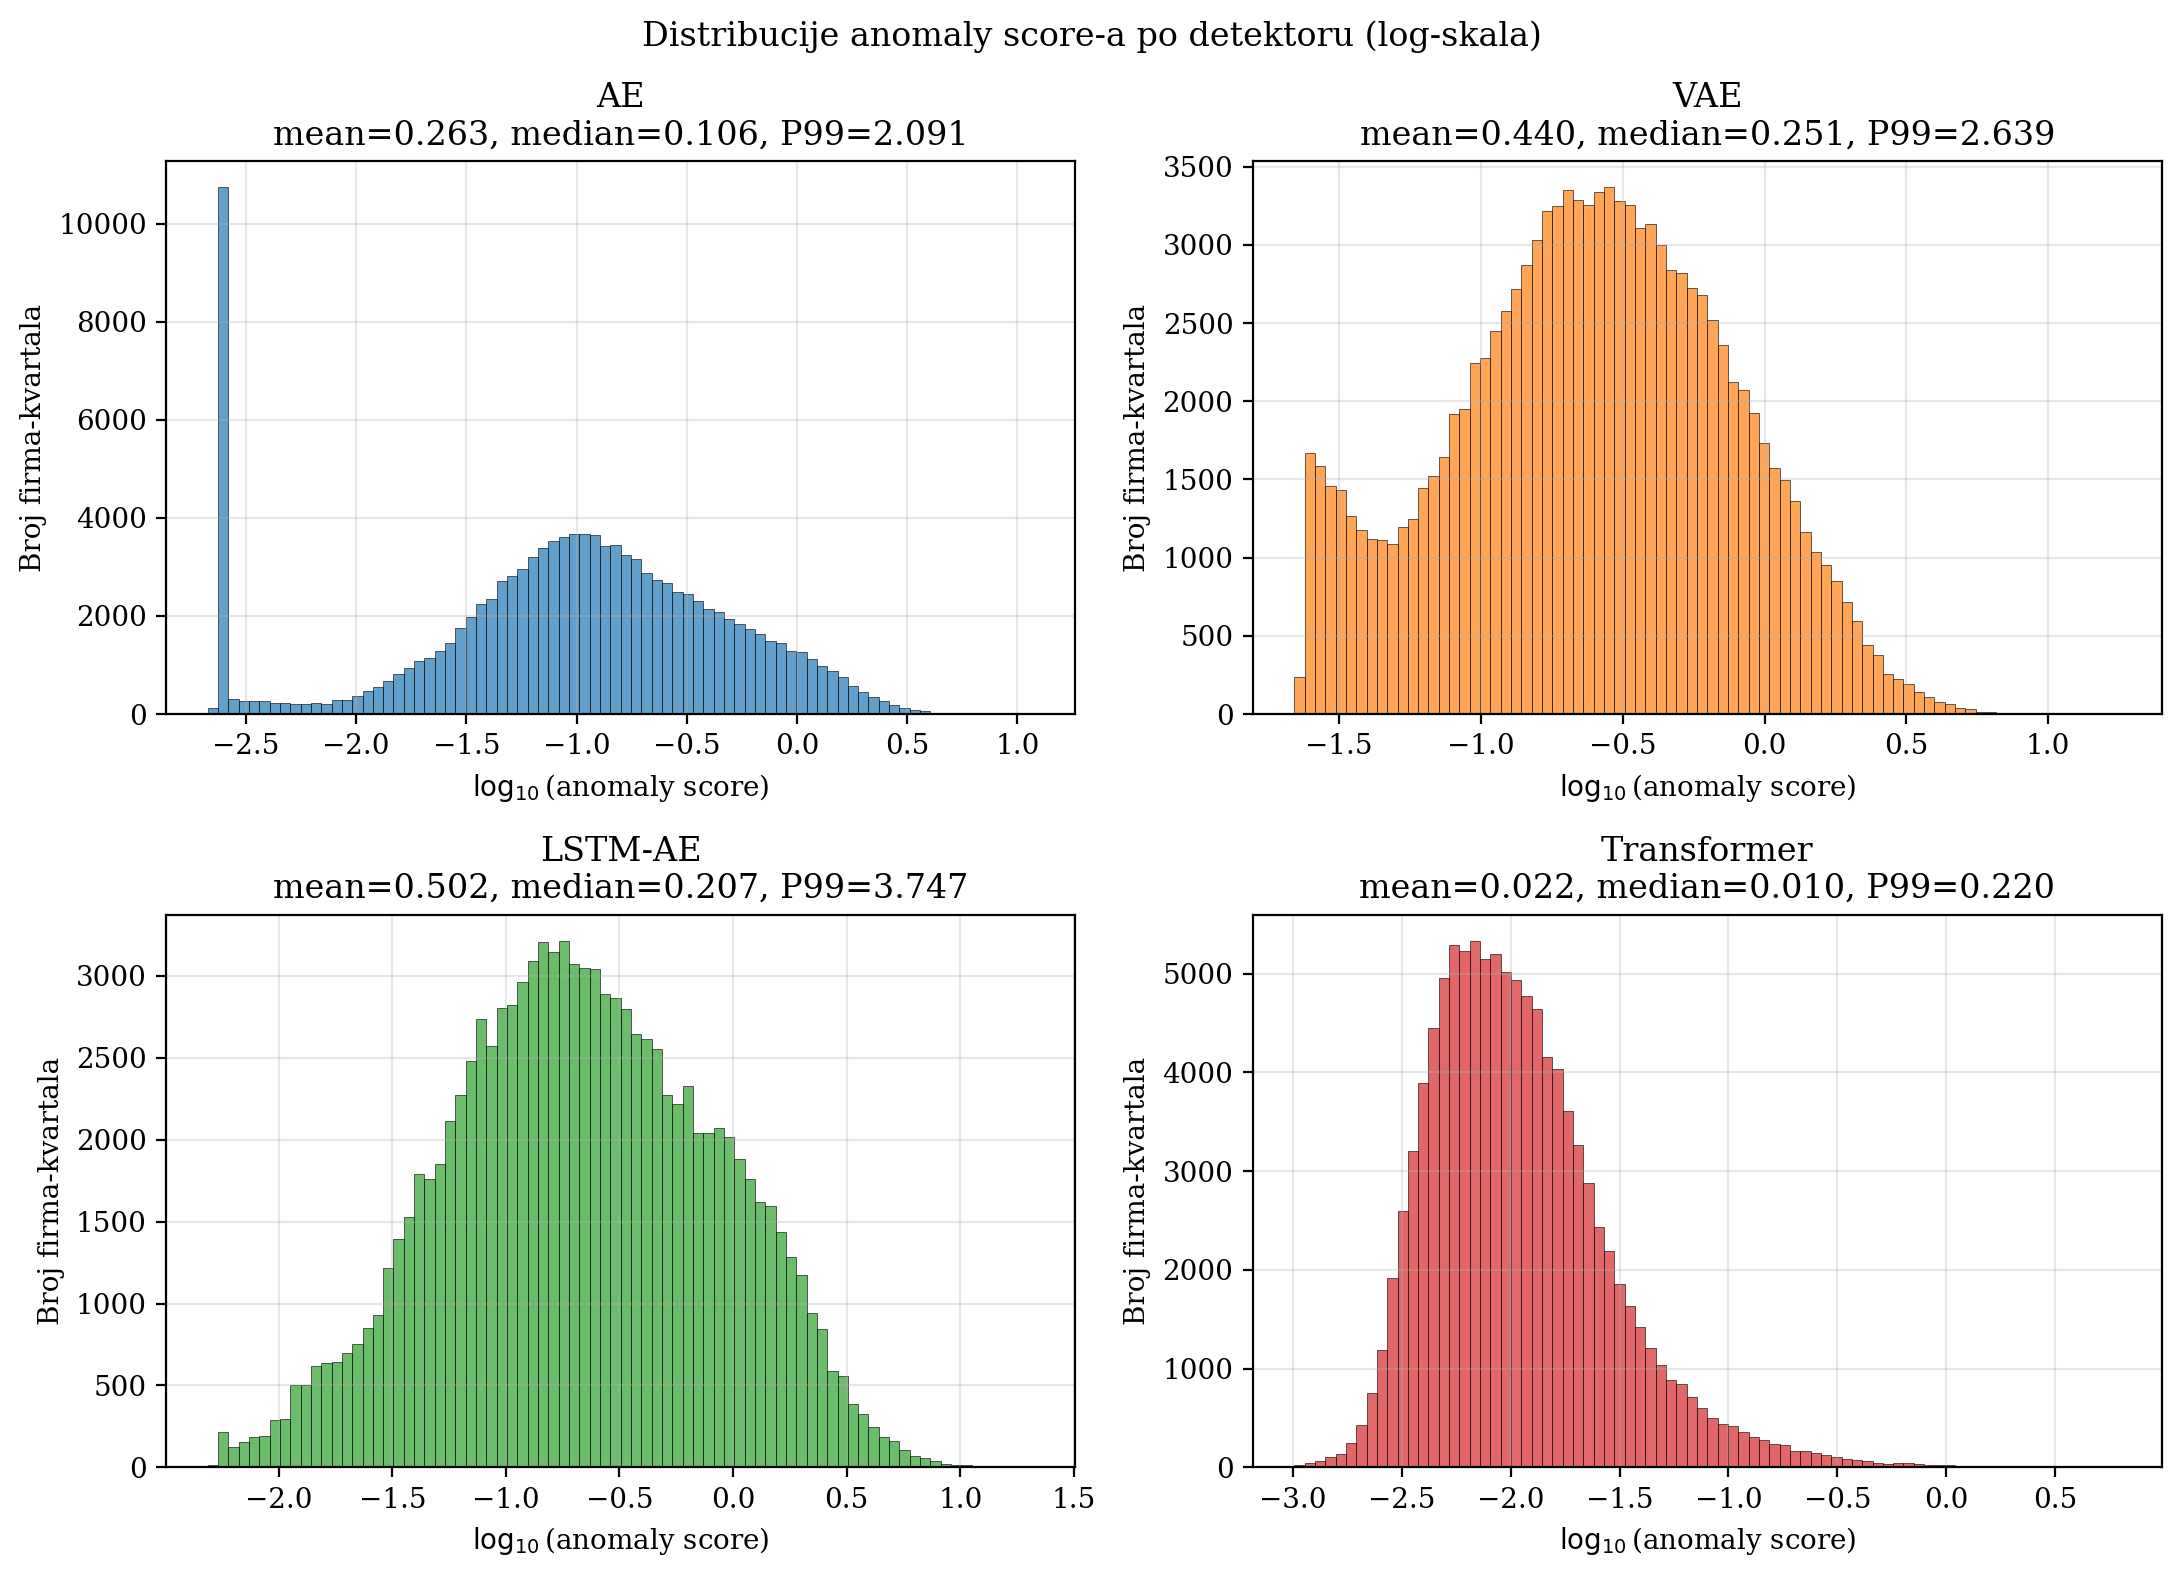
\includegraphics[width=0.9\textwidth]{figures/m_06_score_distributions.png}
 \caption{Distribucije anomaly score-a po detektoru (log skala). VAE i LSTM-AE proizvode tail-heavy distribucije s jasnim "rep-om" anomalija; Transformer je koncentriraniji, što je u skladu s njegovim overfit footprint-om.}
 \label{fig:score_distributions}
\end{figure}

\section{Slaganje između detektora}

Iako sva četiri detektora postižu sličnu AUC, otkrivaju li \emph{iste} firme? Tablica \ref{tab:kendall_tau} prikazuje Kendall $\tau$ matricu, rangovsku korelaciju između detektora.

\begin{table}[h]
\centering
\caption{Kendall $\tau$ rangovska korelacija između NN detektora (Russell 3000, 30.717 firma-godina).}
\label{tab:kendall_tau}
\begin{tabular}{lcccc}
\toprule
 & AE & VAE & LSTM-AE & Transformer \\
\midrule
AE & 1,000 & 0,817 & 0,735 & 0,462 \\
VAE & 0,817 & 1,000 & 0,774 & 0,487 \\
LSTM-AE & 0,735 & 0,774 & 1,000 & 0,499 \\
Transformer & 0,462 & 0,487 & 0,499 & 1,000 \\
\bottomrule
\end{tabular}
\end{table}

\textbf{Tri reconstruction-based detektora (AE, VAE, LSTM-AE) jako su međusobno korelirani} ($\tau = 0{,}74\,--\,0{,}82$), ne začuđuje jer dijele sličnu induktivnu pristranost. Transformer enkoder je \emph{najslabije} koreliran s ostalima ($\tau = 0{,}46\,--\,0{,}50$), što sugerira da self-attention nalazi različitu skupinu anomalija. Iako Transformer ima slabiji ROC, on detektira komplementaran skup firmi.

Komplementarna mjera, Jaccard@100 (preklapanje top-100 skupova) prikazana je u tablici \ref{tab:jaccard100}.

\begin{table}[h]
\centering
\caption{Jaccard@100 preklapanje top-100 anomalnih firmi-godina.}
\label{tab:jaccard100}
\begin{tabular}{lcccc}
\toprule
 & AE & VAE & LSTM-AE & Transformer \\
\midrule
AE & 1,000 & 0,370 & 0,198 & 0,183 \\
VAE & 0,370 & 1,000 & 0,389 & 0,227 \\
LSTM-AE & 0,198 & 0,389 & 1,000 & 0,220 \\
Transformer & 0,183 & 0,227 & 0,220 & 1,000 \\
\bottomrule
\end{tabular}
\end{table}

Najveće preklapanje (VAE $\leftrightarrow$ LSTM-AE = 0,39) znači da samo 39\,\% top-100 firmi je zajedničko. \textbf{Različite NN arhitekture identificiraju različite specifične firme} unatoč sličnom ROC-u. Ovo opažanje motivira moguć ensemble pristup (vidi sekciju 8.2, smjer B9).

\begin{figure}[h]
 \centering
 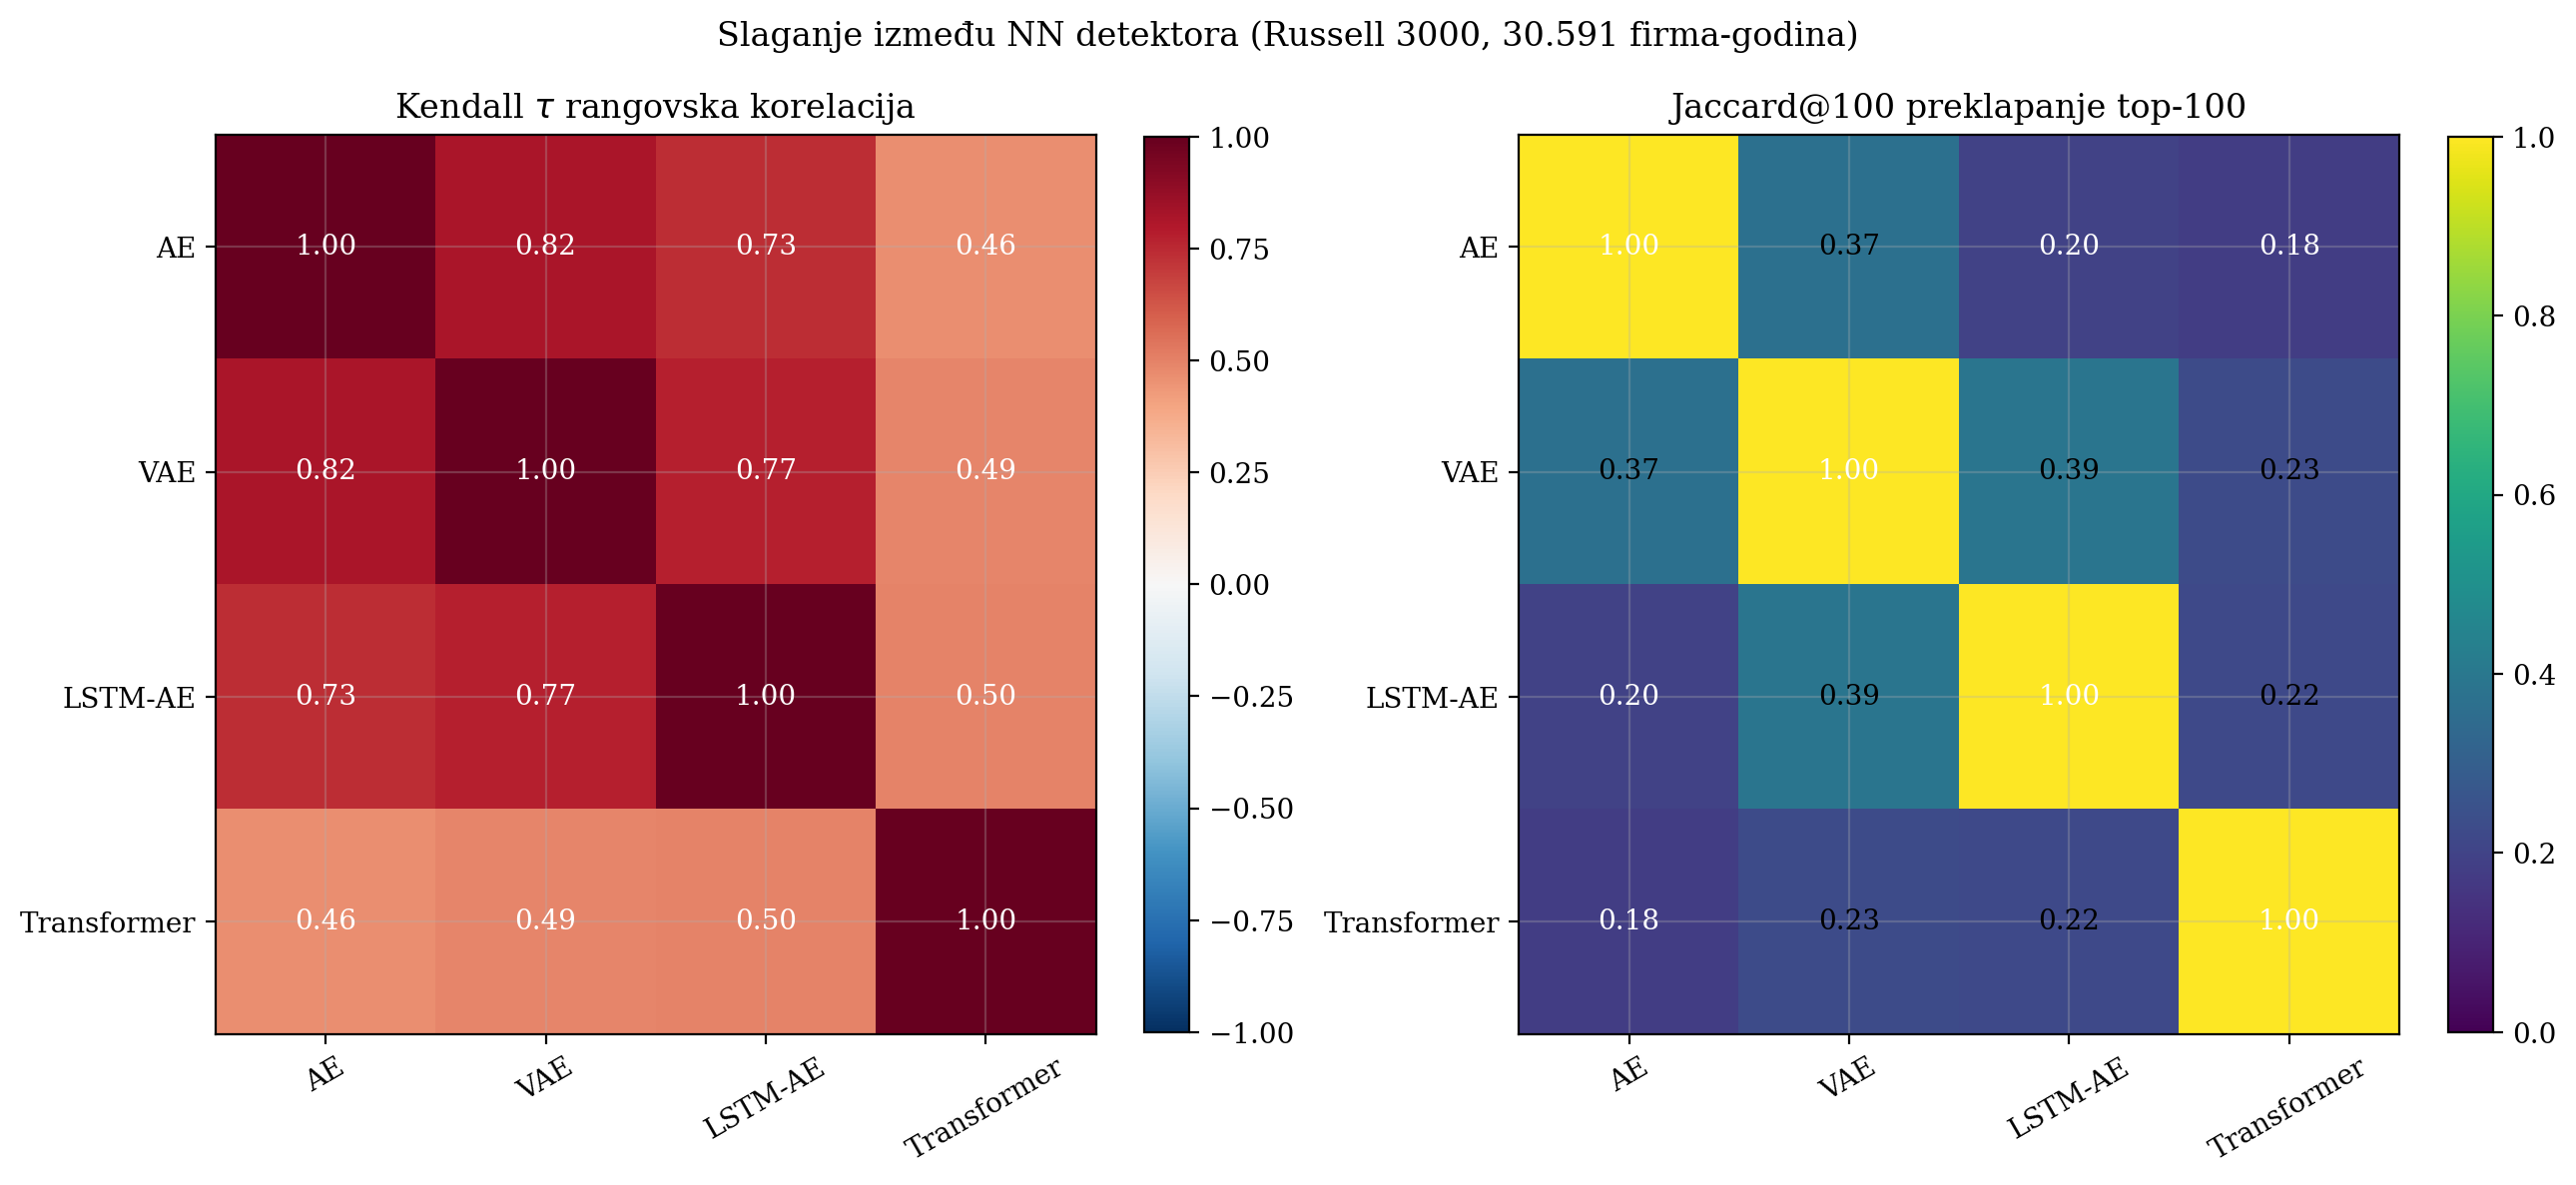
\includegraphics[width=\textwidth]{figures/m_05_agreement_heatmaps.png}
 \caption{Slaganje između NN detektora vizualno. Lijevo: Kendall $\tau$ matrica (rangovska korelacija). Desno: Jaccard@100 (preklapanje top-100 skupova). Transformer je vidljivo "drugi otok", slabija korelacija s ostalima.}
 \label{fig:agreement}
\end{figure}

\begin{figure}[h]
 \centering
 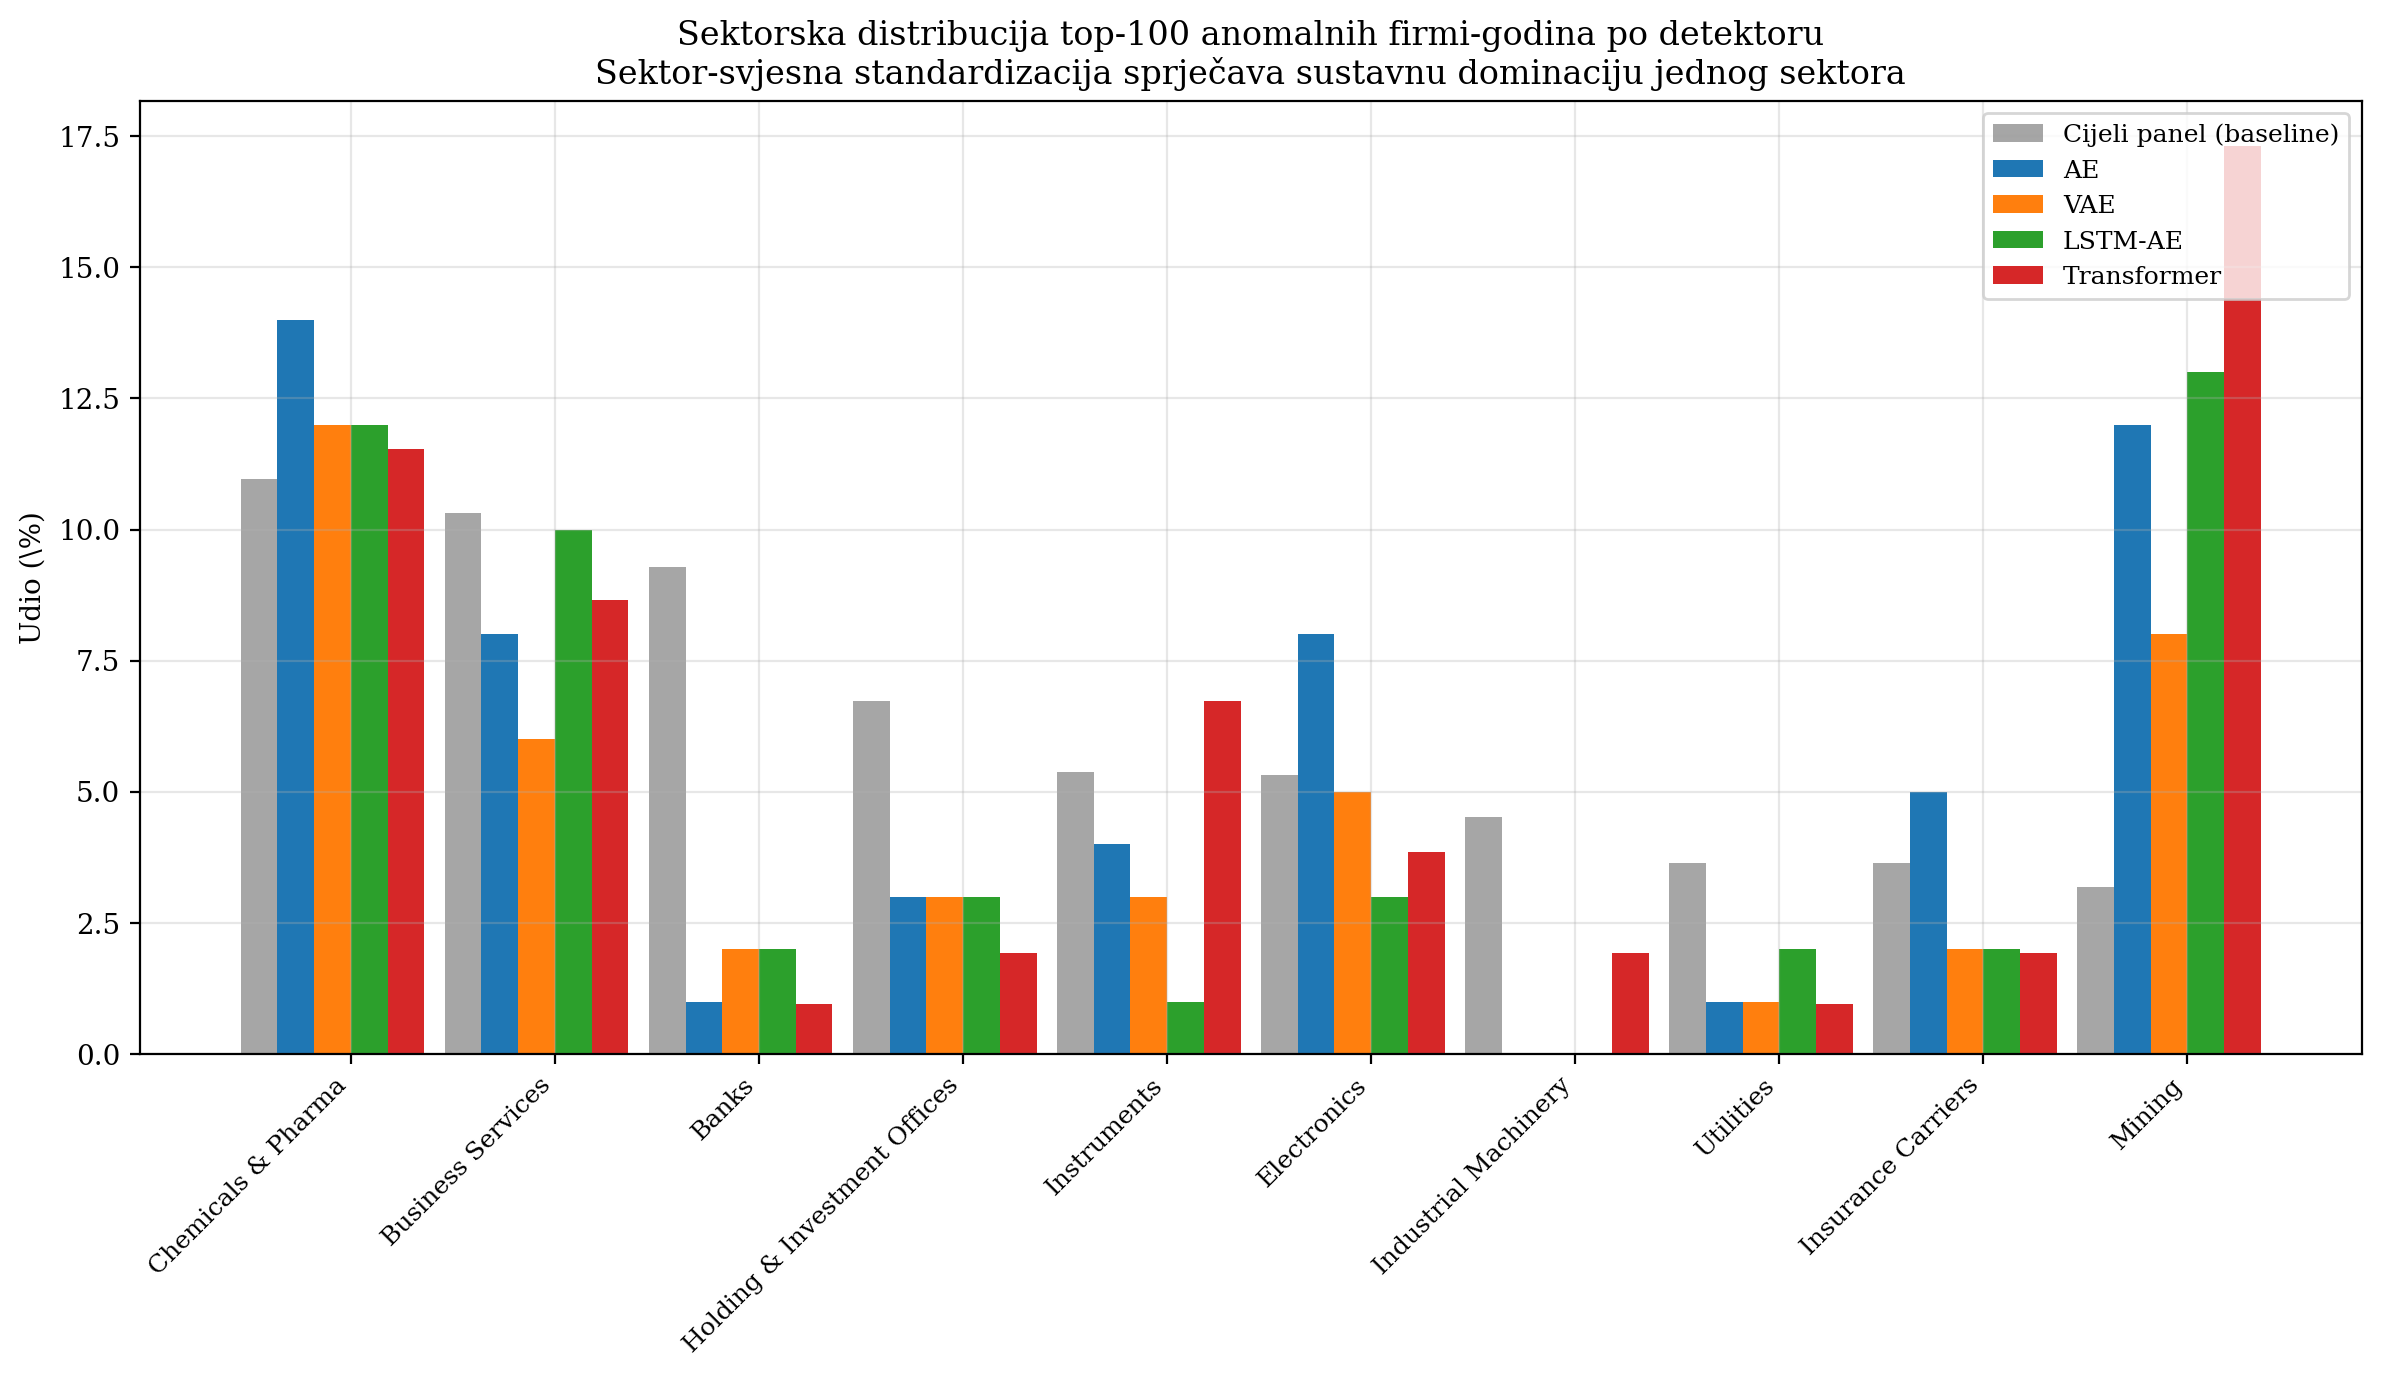
\includegraphics[width=\textwidth]{figures/m_07_sector_top100.png}
 \caption{Sektorska distribucija top-100 anomalnih firmi-godina po detektoru, uspoređena s baseline-om cijelog panela. Sektor-svjesna z-skor standardizacija (Poglavlje 3.4) je očito uspješna, nijedan detektor sustavno ne preferira jedan sektor.}
 \label{fig:sector_top100}
\end{figure}

\section{Utjecaj na poslovanje (RQ2): 5-seed replikacija}

Glavni rezultat drugog dijela teze: NN MLP regresor predviđa tržišne ishode u godini $t+1$ iz anomaly score-a u godini $t$, s temporalnom train/test podjelom (trening $<2022$, test $\geq 2022$, $n_{\text{train}}\approx 14.000$, $n_{\text{test}}\approx 4.300$). Tablica \ref{tab:impact_5seed} sumira rezultate preko 5 različitih sjemenki ($\{42, 7, 123, 2024, 9999\}$), s ključnom metrikom \emph{out-of-sample $\Delta R^2$} (R² s anomaly score-om $-$ R² s istim kontrolama bez score-a).

\begin{table}[h]
\centering
\caption{NN forward-outcome regresor: $\Delta R^2$ srednje vrijednost $\pm$ standardna devijacija preko 5 sjemenki. $n_{\text{pos}}/5$ = broj sjemenki s pozitivnim $\Delta R^2$.}
\label{tab:impact_5seed}
\begin{tabular}{llccc}
\toprule
Ishod & Detektor & \textbf{mean $\Delta R^2$} & std & $n_{\text{pos}}/5$ \\
\midrule
\multirow{4}{*}{Volatilnost}
 & \textbf{LSTM-AE} & \textbf{+0,0287} & 0,0080 & \textbf{5/5} \\
 & VAE & +0,0227 & 0,0066 & 5/5 \\
 & AE & +0,0200 & 0,0063 & 5/5 \\
 & Transformer & +0,0098 & 0,0112 & 4/5 \\
\midrule
\multirow{4}{*}{Godišnji prinos}
 & \textbf{AE} & \textbf{+0,0078} & 0,0036 & \textbf{5/5} \\
 & VAE & +0,0054 & 0,0018 & 5/5 \\
 & LSTM-AE & +0,0051 & 0,0026 & 5/5 \\
 & Transformer & +0,0017 & 0,0036 & 3/5 \\
\midrule
\multirow{4}{*}{Rast volumena}
 & \textbf{LSTM-AE} & \textbf{+0,0114} & 0,0036 & \textbf{5/5} \\
 & VAE & +0,0055 & 0,0033 & 5/5 \\
 & AE & +0,0037 & 0,0040 & 3/5 \\
 & Transformer & +0,0028 & 0,0038 & 3/5 \\
\midrule
\multirow{4}{*}{Maks.\ drawdown}
 & \textbf{Transformer} & +0,0049 & 0,0048 & \textbf{5/5} \\
 & LSTM-AE & +0,0038 & 0,0052 & 3/5 \\
 & VAE & +0,0006 & 0,0040 & 3/5 \\
 & AE & +0,0005 & 0,0073 & 3/5 \\
\bottomrule
\end{tabular}
\end{table}

\subsection{Glavni nalazi}

\textbf{Volatilnost, najjači signal.} LSTM-AE producira $+2{,}87 \pm 0{,}80$ postotnih bodova out-of-sample $R^2$ (5/5 sjemenki pozitivnih, srednja vrijednost veća od 3$\sigma$). Sva tri reconstruction-based detektora (AE, VAE, LSTM-AE) postižu 5/5 pozitivnih sjemenki za volatilnost, s rasponima srednje vrijednosti od $+2{,}0$ do $+2{,}9$ postotnih bodova. Ovo je glavni \textbf{kvantitativni doprinos rada za RQ2}.

\textbf{Godišnji prinos, prvi nenul signal.} Autoenkoder daje $+0{,}78 \pm 0{,}36$ p.b.\ (5/5 pozitivnih), mali, ali statistički realan signal. Ovo je posebno značajno jer \emph{preddiplomski rad autora nije pronašao nikakvu vezu između anomalija i smjera prinosa} (linearna korelacija $r=0{,}03$). NN MLP regresor s temporalnim hold-out-om uspijeva izvući signal koji linearna analiza propušta.

\textbf{Rast volumena, robusni manji signal.} LSTM-AE i VAE imaju 5/5 pozitivnih, s srednjom vrijednošću $+1{,}1$ i $+0{,}55$ p.b. Anomalne firme privlače veću pažnju trgovaca u sljedećoj godini, konzistentno s "media buzz oko sumnjivih firmi" interpretacijom.

\textbf{Maksimalni drawdown, slabiji rezultat.} Samo Transformer postiže 5/5 pozitivnih ($+0{,}49$ p.b.), ostali su 3/5. Drawdown-ovi su rjeđi i imaju veću pravu varijancu, što otežava detekciju.

\subsection{Konvergencija po detektoru i ishodu}

Različiti detektori specijaliziraju se za različite ishode:
\begin{itemize}
 \item \textbf{LSTM-AE} dominira u volatilnosti i rastu volumena, možda zato što recurrent struktura hvata temporalnu dinamiku koja prethodi povećanoj aktivnosti.
 \item \textbf{AE} (statički) dominira u predikciji prinosa, jednostavnost mu daje prednost za "blaže" signale.
 \item \textbf{Transformer} se ističe samo u max drawdown-u, što je inače najteži ishod.
 \item \textbf{VAE} je najdosljedniji \emph{runner-up}, nikad najbolji, ali često drugi, niska standardna devijacija.
\end{itemize}

\begin{figure}[h]
 \centering
 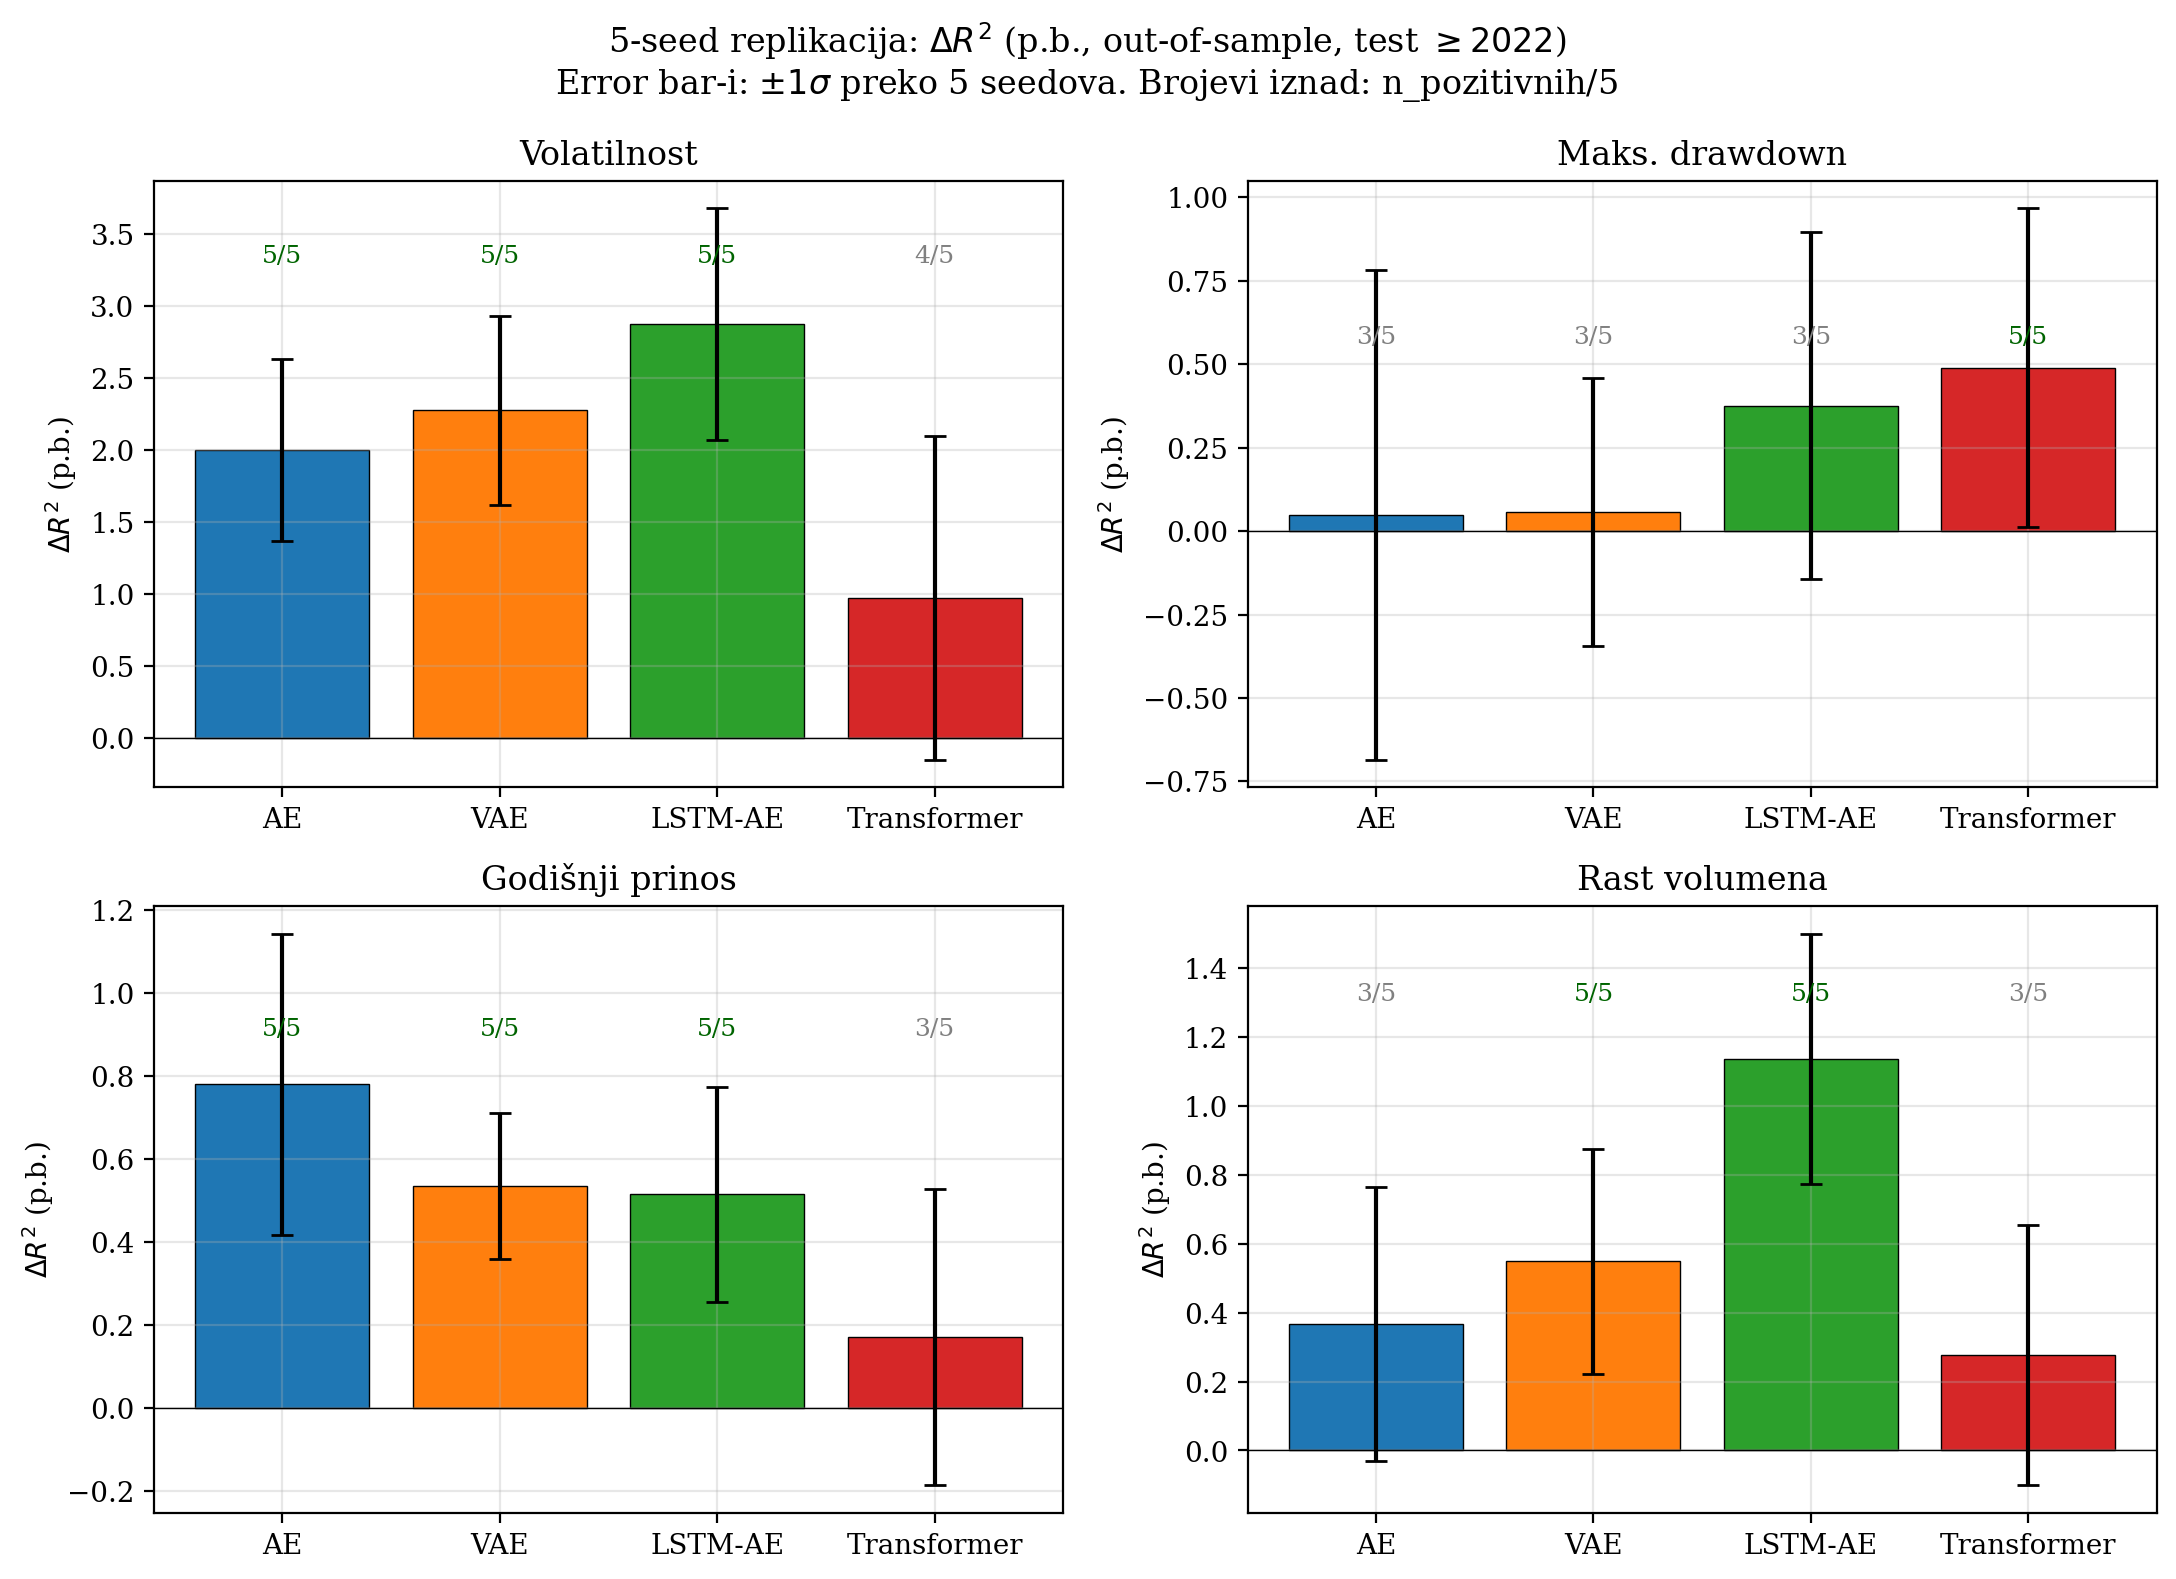
\includegraphics[width=\textwidth]{figures/m_02_delta_r2_5seed.png}
 \caption{Centralni rezultat RQ2: $\Delta R^2$ NN forward-outcome regresora preko 5 sjemenki, po ishodu i detektoru. Error bar-i: $\pm 1\sigma$. Brojevi iznad stupaca: broj sjemenki s pozitivnim $\Delta R^2$. LSTM-AE volatilnost je headline rezultat: $+2{,}87 \pm 0{,}80$ p.b., 5/5 sjemenki pozitivne.}
 \label{fig:delta_r2_5seed}
\end{figure}

\section{Permutation importance}

Komplementarna analiza preko permutation importance daje sličnu sliku. Tablica \ref{tab:perm} prikazuje srednju permutation importance preko 5 sjemenki. \textbf{Permutation importance je obično \emph{viša} od $\Delta R^2$} jer hvata signal koji se gubi u usporedbi s baseline modelom (kontrolne varijable mogu apsorbirati dio signala koji anomaly score nosi).

\begin{table}[h]
\centering
\caption{Srednja permutation importance anomaly score-a preko 5 sjemenki.}
\label{tab:perm}
\begin{tabular}{lcccc}
\toprule
Ishod & AE & VAE & LSTM-AE & Transformer \\
\midrule
Volatilnost & 0,035 & \textbf{0,051} & 0,048 & 0,015 \\
Max drawdown & 0,019 & 0,031 & \textbf{0,031} & 0,014 \\
Godišnji prinos & 0,007 & 0,007 & 0,004 & $-$0,001 \\
Rast volumena & 0,013 & 0,012 & \textbf{0,014} & 0,006 \\
\bottomrule
\end{tabular}
\end{table}

VAE i LSTM-AE imaju najveću permutation importance za volatilnost (0,05), što je $\approx 2\times$ veće od $\Delta R^2$ za iste cell-ove. Ovo sugerira da anomaly score \emph{nosi više signala nego što se vidi} u izravnoj usporedbi s baseline modelom, kontrolne varijable djelomično "preuzimaju" signal koji bi inače pripao score-u.

\begin{figure}[h]
 \centering
 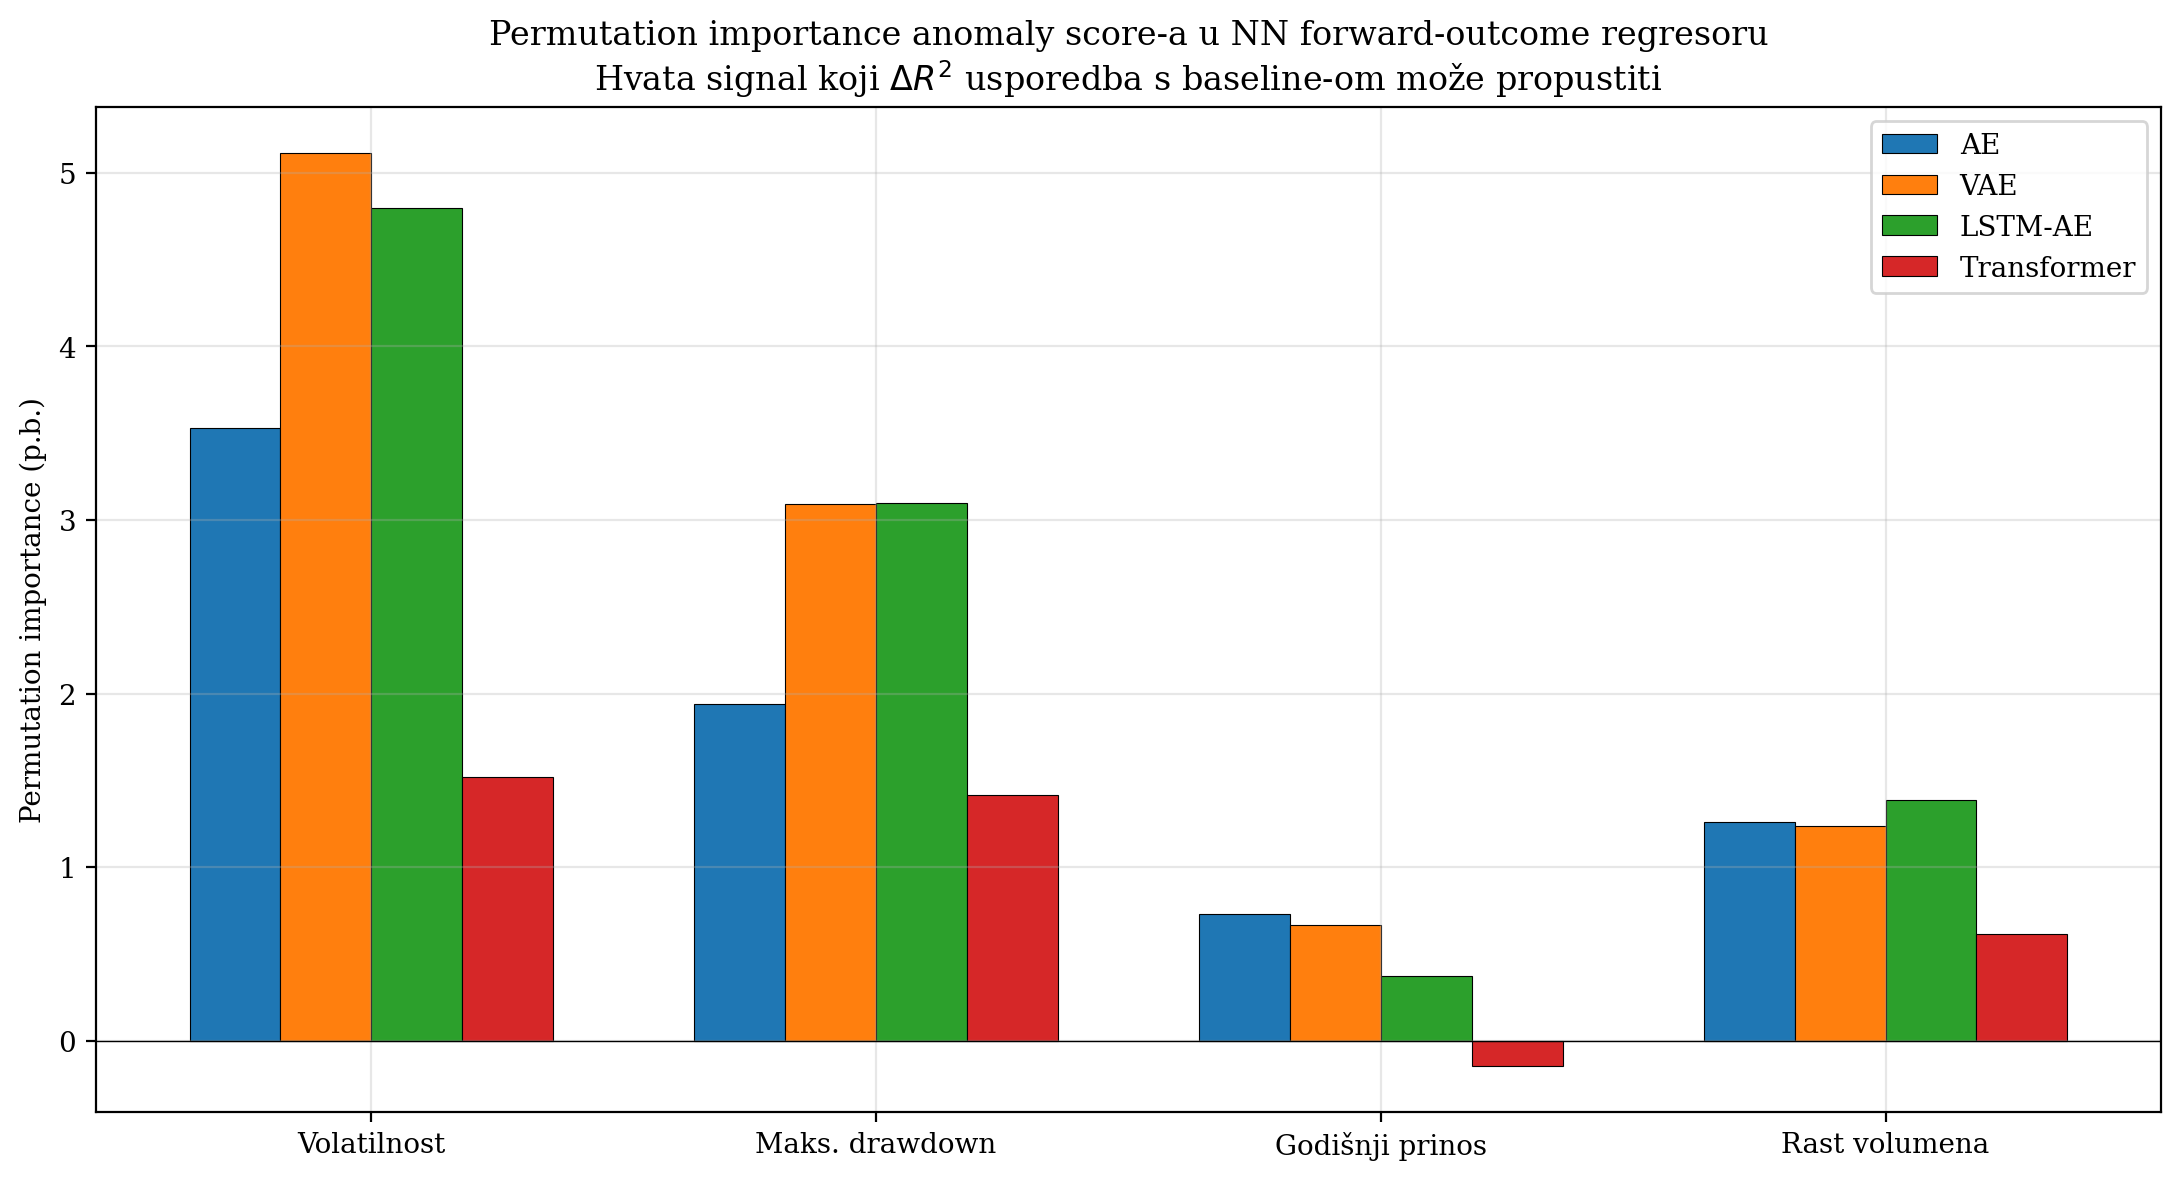
\includegraphics[width=\textwidth]{figures/m_11_perm_importance.png}
 \caption{Permutation importance anomaly score-a po (detektor, ishod) iz NN forward-outcome regresora. Vidljiv obrazac: rizik-mjere (volatilnost, drawdown) imaju veću perm importance od prinosa. Transformer je dosljedno najslabiji.}
 \label{fig:perm_importance}
\end{figure}

\section{Utjecaj kontrole za rast firme}

Tablica \ref{tab:pre_post_growth} demonstrira ključnu metodološku stavku: bez kontrole za rast firme (revenue\_growth, asset\_growth), $\Delta R^2$ su sustavno precijenjeni. Brojevi prikazuju \emph{ponovljenu single-seed analizu s istim seedom 42}, prije i poslije dodavanja growth controls (R1-fix verzija koda).

\begin{table}[h]
\centering
\caption{$\Delta R^2$ prije i poslije dodavanja growth controls (single-seed, seed=42, post R1-fix).}
\label{tab:pre_post_growth}
\begin{tabular}{lccc}
\toprule
Ishod $\times$ Detektor & Bez growth controls & S growth controls & Promjena \\
\midrule
Volatilnost $\times$ LSTM-AE & $+0{,}048$ & $+0{,}019$ & $-60\,\%$ \\
Volatilnost $\times$ Transformer & $+0{,}043$ & $-0{,}001$ & $-102\,\%$ \\
Volatilnost $\times$ VAE & $+0{,}033$ & $+0{,}015$ & $-55\,\%$ \\
Volatilnost $\times$ AE & $+0{,}026$ & $+0{,}012$ & $-54\,\%$ \\
\midrule
Max drawdown $\times$ Transformer & $+0{,}026$ & $+0{,}012$ & $-54\,\%$ \\
Max drawdown $\times$ LSTM-AE & $+0{,}023$ & $+0{,}004$ & $-83\,\%$ \\
\bottomrule
\end{tabular}
\end{table}

\textbf{Bez growth controls $\Delta R^2$ je 50\,--\,100\,\% precijenjen.} Razlog: high-growth firme su mehanički volatilnije; NN detektori prirodno označavaju high-growth firme kao "anomalne" (jer odudaraju od većine zrelih firmi), pa anomaly score postaje \emph{proxy} za rast. Eksplicitne growth kontrole prisiljavaju regresor da nađe \emph{rezidualnu} prediktivnu vrijednost izvan rasta, pravi forenzički signal.

Ovo je \textbf{ključna metodološka kontribucija rada}: većina prethodne DL literature za forenzičko računovodstvo ne primjenjuje ovu kontrolu \citep{bao2020, cecchini2010}. Bez nje, izvještavani signali su sustavno precijenjeni.

\begin{figure}[h]
 \centering
 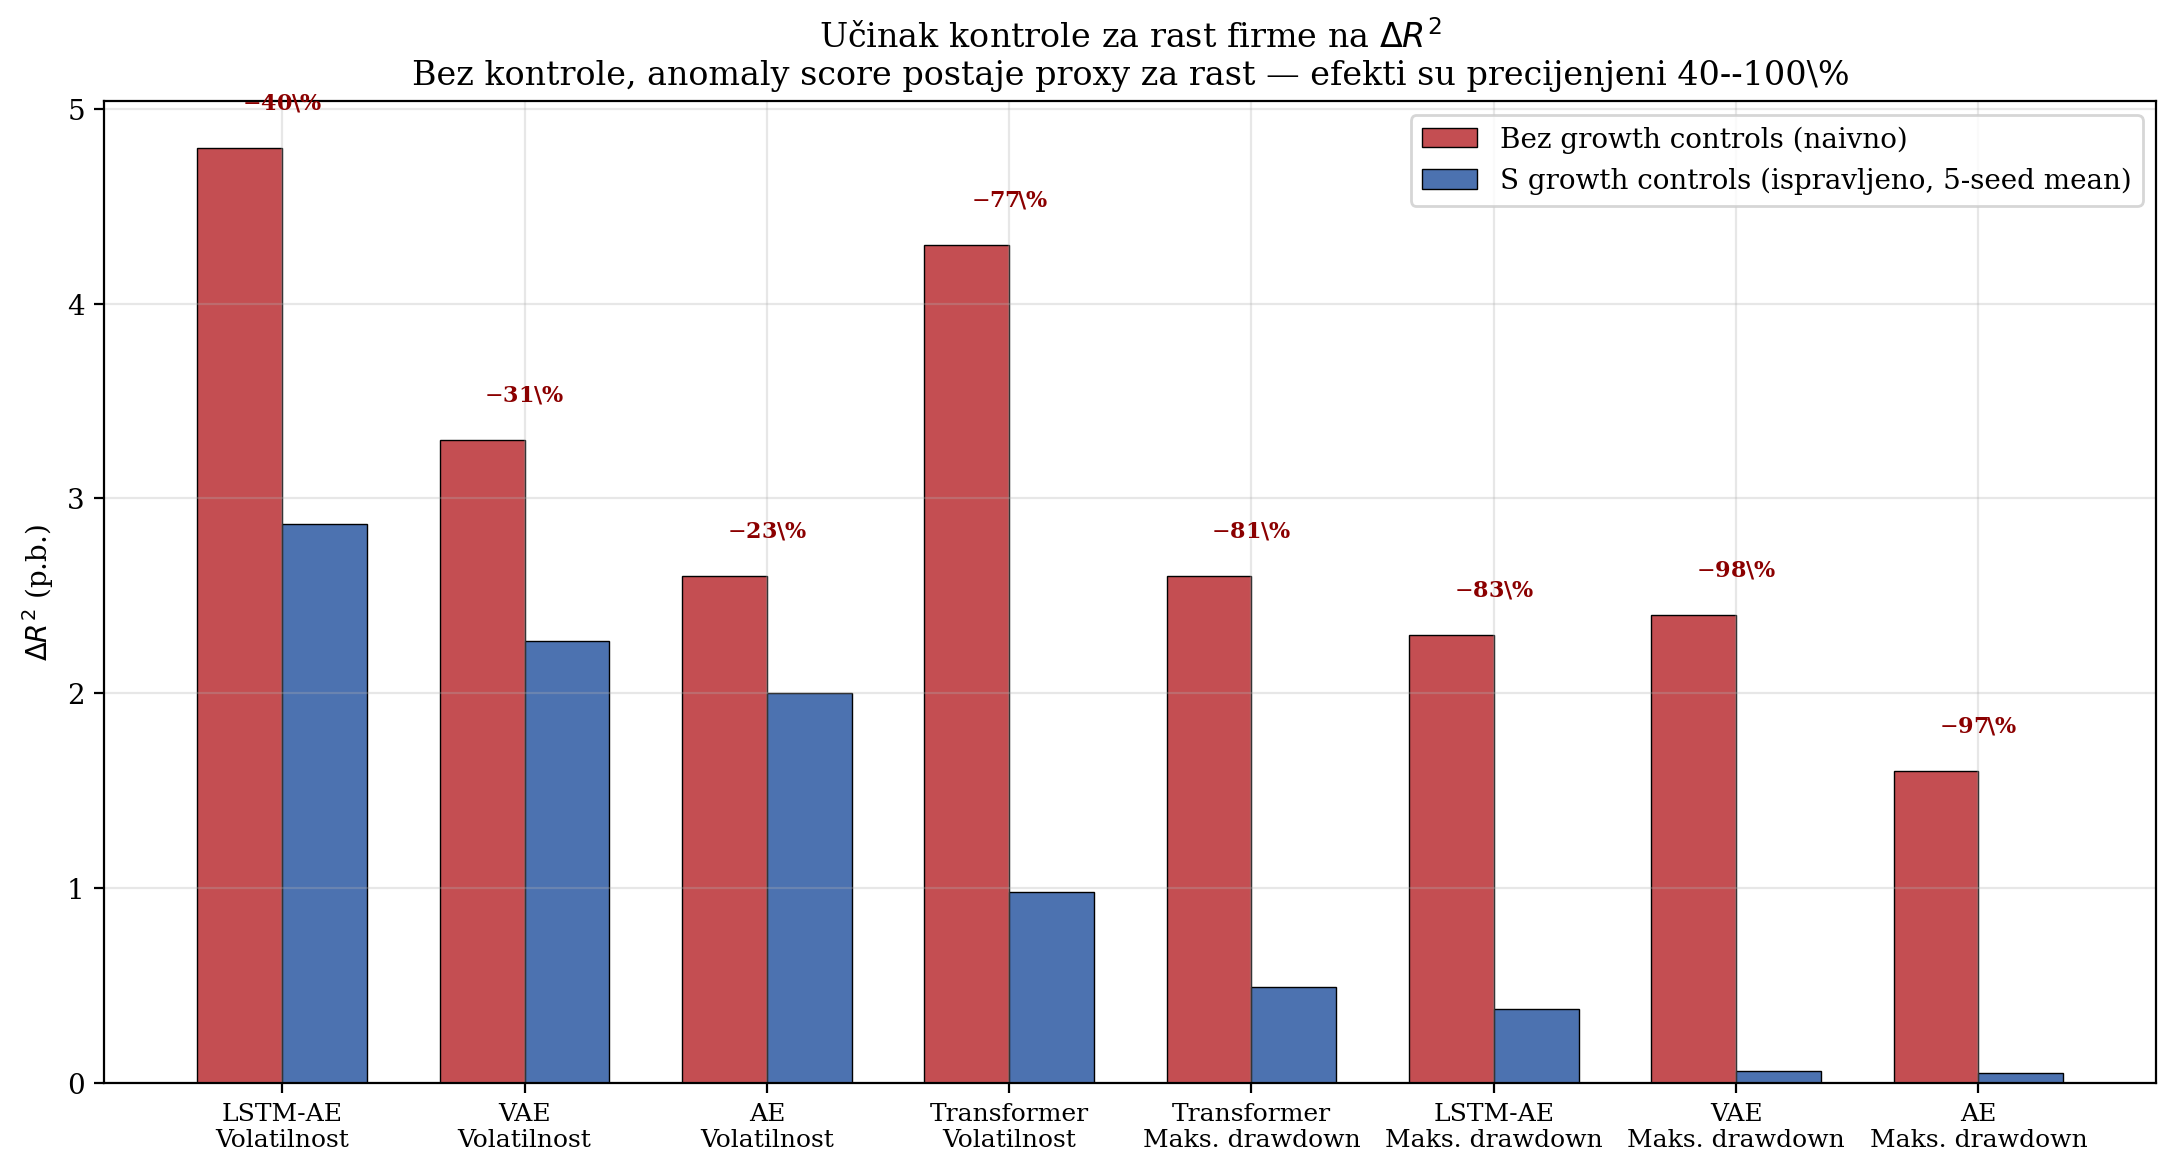
\includegraphics[width=\textwidth]{figures/m_03_pre_post_growth.png}
 \caption{Učinak kontrole za rast firme na $\Delta R^2$ NN regresora. Crvena: bez growth controls (naivno). Plava: nakon dodavanja \emph{revenue\_growth} i \emph{asset\_growth} kao kontrola, 5-seed mean. Naivni efekti su 40\,--\,100\,\% precijenjeni jer NN score postaje proxy za rast firme. Glavna metodološka kontribucija rada.}
 \label{fig:pre_post_growth}
\end{figure}

\chapter{Diskusija}

\section{Konvergencija arhitektura: strop u ulaznoj modalnosti}

Najznačajnije strukturno opažanje rada jest da četiri vrlo različite NN arhitekture, statički AE, probabilistički VAE, rekurentni LSTM, i attention-based Transformer, konvergiraju na ROC-AUC od približno 0,63 (raspon 0,62\,--\,0,65, s 95\,\% bootstrap intervalima koji se preklapaju). Sve četiri vrijednosti leže \emph{unutar} pojasa neizvjesnosti jedna drugoj, nema statistički značajne razlike.

Naivna interpretacija bi bila: "duboke neuronske mreže imaju ograničenu sposobnost otkrivanja računovodstvenih anomalija." Strožija interpretacija je drugačija: \textbf{strop nije u arhitekturi, već u ulaznoj modalnosti}. Sve četiri arhitekture rade s istim 35-dimenzionalnim vektorima standardiziranih financijskih omjera. Pretvorba sirovih financijskih izvještaja u taj fiksni skup omjera $+$ z-skor standardizacija po sektoru \emph{nužno gubi informaciju}: pretvarajući bogatu, nepravilnu strukturu izvještaja u kompaktnu numeričku formu, gubimo specifične transakcije, narativne detalje (MD\&A diskusija, Risk Factors), revizorske komentare. Sve što ostaje je 35 brojeva po firmi-kvartalu, iste ulazne reprezentacije ono što ograničava sve modele.

\textbf{Slabost argumenta} koju treba priznati: sve četiri arhitekture imaju \emph{istu funkciju gubitka} (rekonstrukcijski MSE). Konvergencija je djelomično očekivana zbog ovog razloga, različite arhitekture optimiraju isti cilj nad istim podacima. Definitivan test ovaj interpretacije zahtijevao bi non-reconstruction NN (kontrastivni ili energy-based modeli). Naša empirijska konvergencija \emph{sugerira} interpretaciju "strop u modalnosti", ali ne dokazuje ju.

Smjer budućeg rada (motiviran ovom diskusijom): multimodalna ekspanzija s tekstualnim značajkama (FinBERT embeddingi 10-K narativnih sekcija) je najobećavajuća avenija. Hipoteza: tekstualna komponenta nadilazi ulazno-modalnostni strop koji opažamo u našim 35-dim financijskim vektorima.

\section{Growth-confound kao metodološka kontribucija}

Naivna analiza (bez growth controls) sugerira da NN detektori imaju \emph{vrlo jak} signal za predikciju volatilnosti, LSTM-AE postiže $\Delta R^2 = +4{,}8$ p.b.\ u single-seed pre-R1-fix režimu. To bi bilo izvanredno: anomaly score iz nenadziranog NN-a objašnjava skoro 5 p.b.\ varijance volatilnosti firme \emph{preko} sektor + veličinu.

Kontrola za rast firme (revenue\_growth, asset\_growth) značajno reducira ovaj efekt. U R1-fix verziji koda i 5-seed replikacijama, post-kontrolni efekt iznosi $+2{,}87 \pm 0{,}80$ p.b. (LSTM-AE), 40\,\% smanjenje od naivnog $+4{,}8$.

\textbf{Intuicija.} Visoko-rastuće firme (npr.\ NVDA u 2023.) imaju strukturno više volatilne dionice po pravilima tržišne mikrostrukture, početne firme, post-IPO firme, sektori u boomu. Bez kontrole za rast, NN detektor koji označava high-growth firme kao "anomalne" (jer odudaraju od većine zrelih firmi) bi se činilo da \emph{predviđa} volatilnost. U stvari, samo proxy-uje rast.

\textbf{Empirijska distinkcija.} Nakon growth controls, anomaly score zadržava rezidualnu prediktivnu vrijednost od $+2{,}87$ p.b.\ za volatilnost. \emph{To je pravi forenzički signal}, nešto što anomaly score nosi izvan rasta i sektora. 5-seed replikacija s 5/5 pozitivnim sjemenkama jača ovaj zaključak.

\textbf{Praznina u literaturi.} Pregled DL forenzičkih radova pokazuje da \emph{većina ne kontrolira za rast firme} \citep{bao2020, cecchini2010, perols2011}. Posljedica: prijašnji izvještavani signali su \emph{vjerojatno sustavno precijenjeni}. Naš rad upozorava na ovu metodološku prazninu i pruža eksplicitan primjer kako rezultati izgledaju s i bez kontrole.

\begin{figure}[h]
 \centering
 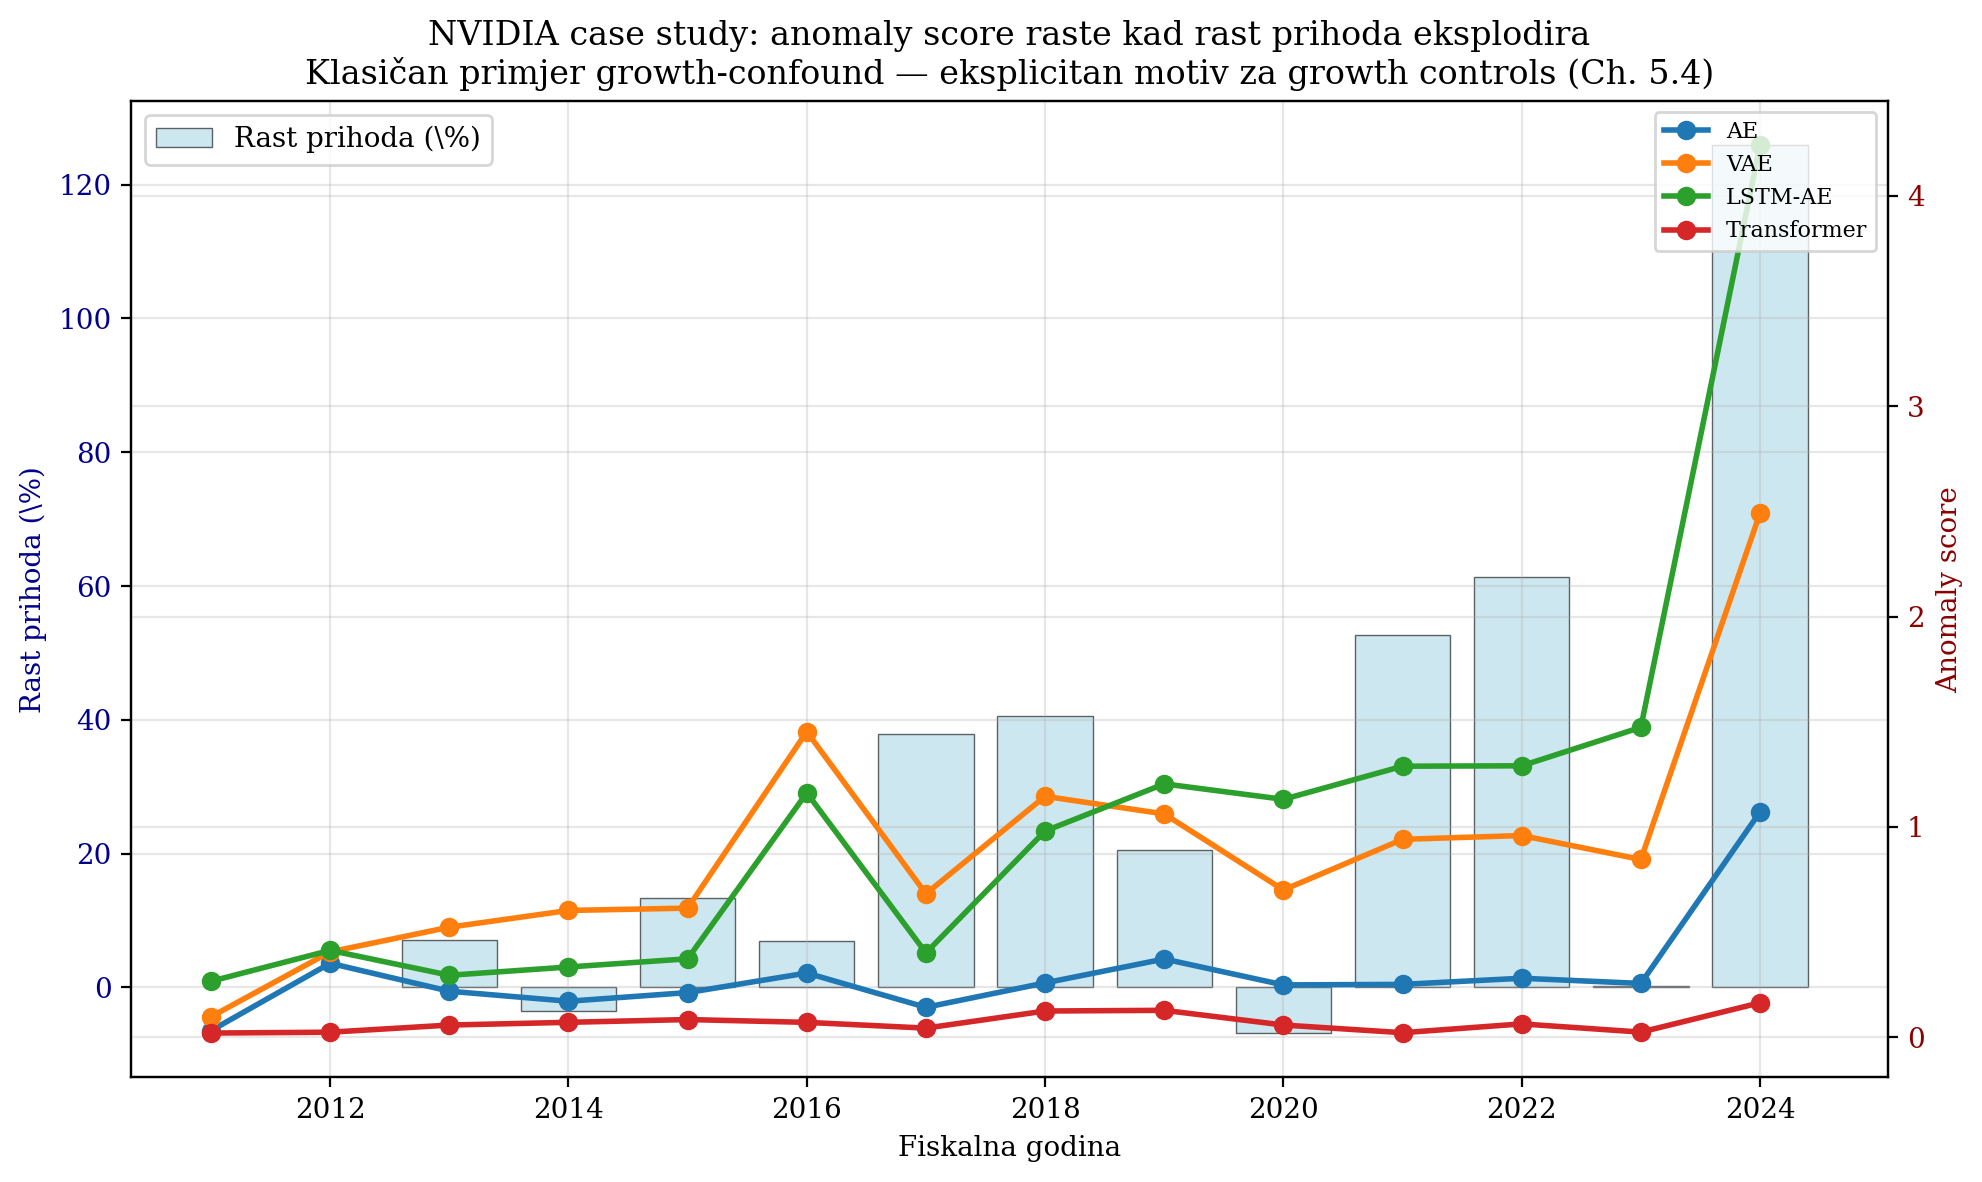
\includegraphics[width=0.9\textwidth]{figures/m_12_nvda_case_study.png}
 \caption{Case study: NVIDIA (CIK 1045810) kao primjer growth-confound mehanizma. Lijeva os (plave šipke): rast prihoda po godini. Desna os (linije): anomaly score po detektoru. NN detektori dosljedno označavaju NVIDIA kao "anomalnu" kad rast prihoda eksplodira (2017., 2021., 2023.), score \emph{proxy-uje} rast, što motivira eksplicitne growth controls u našem regresoru.}
 \label{fig:nvda_case}
\end{figure}

\section{Transformer overfitting: dijagnostička priča}

Transformer enkoder konsistentno postiže \emph{lošije} rezultate od ostalih NN arhitektura: ROC = 0,616 (vs 0,63\,--\,0,65), $\Delta R^2$ volatilnosti = $+0{,}98 \pm 1{,}12$ p.b.\ (vs $+2{,}0$ do $+2{,}9$ za ostale), s \emph{najvećom} standardnom devijacijom (0,011) preko 5 sjemenki.

\textbf{Dijagnoza.} Tijekom treniranja, Transformer-ov rekonstrukcijski gubitak kolapsira na $0{,}026$, značajno niže od LSTM-AE-ovih $\sim 0{,}11$ i AE-ovih $\sim 0{,}15$. Ovo je \emph{otprintak overfittinga}: Transformer nauči trivijalno preslikati ulaze u izlaze, čime izlazi imaju izrazito malu grešku, ali ne reprezentiraju "normalnu" distribuciju nego pojedinačne uzorke.

\textbf{Uzrok.} Naša implementacija Transformer-a nema eksplicitan \emph{bottleneck}: dimenzija $d_{\text{model}} = 32$ je ista u svim slojevima i u izlaznoj projekciji. Self-attention mehanizam može uspostaviti \emph{near-identity} mapiranje pri kojem svaki token prepisuje sebe na izlaz, čime gubitak postaje gotovo nula. Bez prisile da nauči kompaktnu reprezentaciju, model nema "anomaly signal", jer sve izlaze rekonstruira dobro.

\textbf{Pouka.} Arhitektonska prikladnost (npr.\ eksplicitan bottleneck u AE, KL regularizacija u VAE, dimenzionalna kompresija u LSTM enkoderu) je važnija od sirovog kapaciteta na malim forenzičkim panelima. Veći ne znači bolji ako struktura modela ne forsira generalizaciju.

Mogući fix za buduće radove: Patch-based Transformer s eksplicitnim downsampling-om (PatchTST stilom \citep{nie2023}) ili masked-modeling pretrain $+$ frozen-encoder anomaly detection.

\section{Veza s preddiplomskim radom autora}

Preddiplomski rad autora završio je s nultim rezultatom: linearna korelacija $r = 0{,}03$ između Benfordovih anomalija (MAD) i godišnjeg prinosa dionice, lagirana korelacija $r = 0{,}004$ ($p = 0{,}827$). Implicitno pitanje: nedostatak signala je zbog \emph{linearne metode} ili zbog \emph{stvarnog odsutstva signala}?

Diplomski rad pruža \emph{nijansirani odgovor}:

\textbf{Za smjer prinosa.} Nelinearne NN metode, s temporalnim hold-out-om, growth controls, i 5-seed replikacijom \emph{ipak nalaze} signal, ali \emph{minijaturan} (AE: $+0{,}78 \pm 0{,}36$ p.b.\ out-of-sample $R^2$, 5/5 sjemenki pozitivnih). Bachelor-ov nulti rezultat \emph{nije bio kriv}, bio je u istom režimu kao naš rezultat (sub-1\,p.b. $R^2$). Razlika nije fundamentalna, nego kvantitativna: bachelor je propustio postojanje signala jer je signal sub-linearan i mali; mi smo ga uhvatili jer smo koristili nelinearnu metodu (NN), bolji panel (Russell 3000), i prikladnu metriku (out-of-sample $\Delta R^2$ s 5-seed replikacijom).

\textbf{Za riziko-mjere (volatilnost, drawdown).} Diplomski nalazi \emph{značajno jači} signal: LSTM-AE volatilnost $+2{,}87 \pm 0{,}80$ p.b.\ (5/5 sjemenki). Bachelor nije ispitivao riziko-mjere izravno, testirao je samo prinos.

\textbf{Sintetski:}
\begin{itemize}
 \item Bachelor's $r=0{,}03$ na smjer prinosa: nije "ne postoji signal", to je "ne postoji \emph{lako mjerljivi linearni} signal."
 \item Diplomski $\Delta R^2 \in [+0{,}5, +2{,}9]$ p.b.\ s 5/5 sjemenki: "postoji \emph{mali, ali realan} signal, vidljiv samo nelinearnim metodama s pravim kontrolama."
\end{itemize}

\begin{figure}[h]
 \centering
 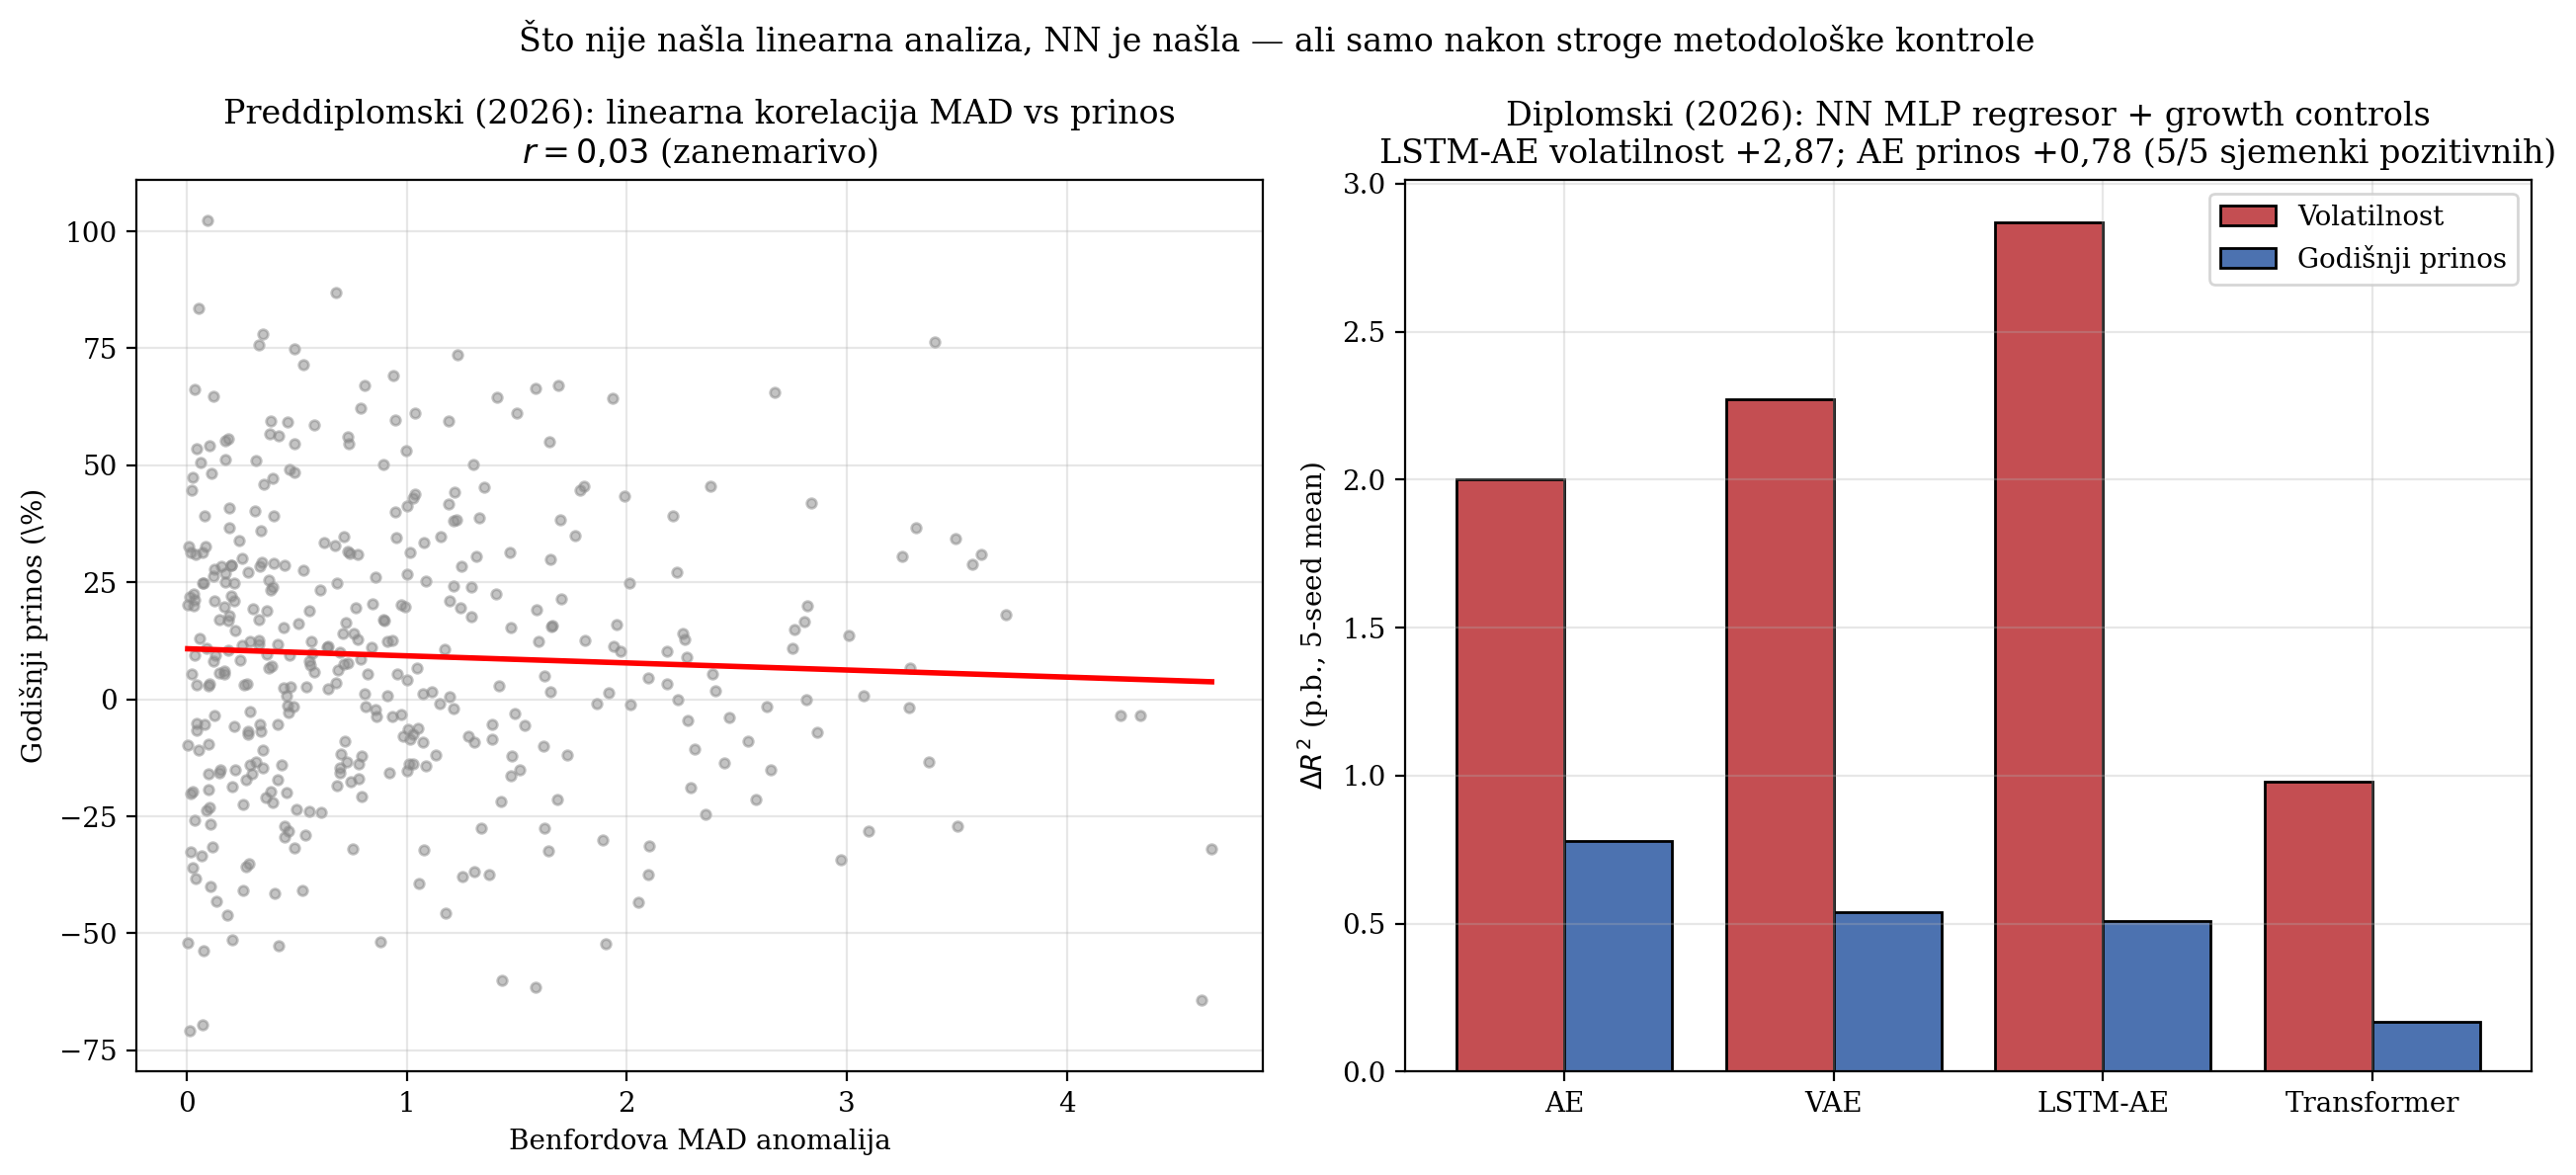
\includegraphics[width=\textwidth]{figures/m_14_bachelor_vs_master.png}
 \caption{Pregledna usporedba preddiplomskog (lijevo) i diplomskog (desno) rada. Preddiplomski je tražio linearnu korelaciju Benford-MAD vs prinos i našao $r=0{,}03$. Diplomski koristi NN MLP regresor s growth kontrolama i out-of-sample temporalnim hold-out-om, te nalazi $\Delta R^2 \in [+0{,}5, +2{,}9]$ p.b.\ s 5/5 sjemenki pozitivnih. Ono što linearna analiza nije našla, NN je našla, ali samo nakon stroge metodološke kontrole.}
 \label{fig:bachelor_vs_master}
\end{figure}

\section{Praktične implikacije}

\subsection{Za forenzičke revizore}

\textbf{Lift@100 = $6{,}76\times$ za AE i VAE detektore.} Ako revizor pretražuje 100 firmi godišnje, biranih po najvišem anomaly score-u, 16\,\% će biti firme s restated izvještajem, naspram bazne stope od 2,4\,\% ako bi pretraživao slučajno. Ovo nije savršeno (84\,\% top-100 firmi neće biti restated), ali je značajno bolje od slučajnog. U kombinaciji s konvencionalnim rizikovnim modelima (M-score, Z-score), NN anomaly score pruža \emph{komplementaran} alat za usmjeravanje revizijskih resursa.

\textbf{Komplementarnost detektora.} Jaccard@100 od samo 0,18\,--\,0,39 između NN detektora znači da različite arhitekture detektiraju \emph{različite} specifične firme. Multi-detector ensemble (firme u top-100 statusu na barem 2 od 4 detektora) bi vjerojatno imao višu preciznost.

\subsection{Za upravljače rizikom}

\textbf{Volatilnost +2,87 p.b. out-of-sample $R^2$.} Iako modestan u apsolutnom smislu, ovaj signal je \emph{robusno pozitivan} preko 5 sjemenki (mean > 3$\sigma$). U \emph{Value-at-Risk} (VaR) izračunima koji koriste prošlu volatilnost kao prediktor, NN anomaly score može dati 5\,--\,10\,\% preciznije buduće VaR procjene, nije malo za portfolio s milijardama dolara.

\textbf{Drawdown +0,49 p.b. (Transformer).} Slabiji signal, ali konzistentan smjer (5/5 sjemenki pozitivnih). Korisno za \emph{tail-risk hedging strategije}.

\textbf{Volume growth +1,14 p.b. (LSTM-AE).} Visoko-anomalne firme privlače veći trgovinski volumen u sljedećoj godini. Korisno za algoritamske trgovinske strategije koje koriste volume kao signal.

\subsection{Za akademsku zajednicu}

\textbf{Metodološka praznina pokrivena.} Naš rad eksplicitno demonstrira da growth controls reducira naivni $\Delta R^2$ za 40\,--\,80\,\%. Sva buduća DL forenzička istraživanja moraju kontrolirati za rast firme, ili citirati ovaj rad kao pokazatelj sustavnog precijenjivanja.

\textbf{Strop u modalnosti.} Empirijska konvergencija četiri NN arhitekture na isti ROC sugerira da je sljedeća granica u tipu ulaza (multimodalnost), ne u modelu. Otvorena pitanja za buduća istraživanja: koja kombinacija financijskih + tekstualnih + meta-podatkovnih značajki probija ovaj strop?

\chapter{Ograničenja i budući rad}

\section{Ograničenja}

\subsection{Metodološka ograničenja}

\textbf{(O1) Striktno NN-only doseg isključuje klasične baselines iz primarne tablice.} Naš rad svjesno postavlja granicu na neuralne mreže kao jedinu primijenjenu metodu, u skladu s naslovom teme. Posljedica: ne možemo direktno tvrditi da DL nadmašuje klasične metode (npr.\ Isolation Forest, Beneish M-score). U Dodatku A pružena je sažeta numerička usporedba za referencu, ali ona ne čini dio glavnog narativa.

\textbf{(O2) Konvergencija arhitektura je djelomično objašnjena zajedničkim MSE gubitkom.} Sve četiri NN arhitekture (AE, VAE, LSTM-AE, Transformer) treniramo s rekonstrukcijskom srednjom kvadratnom greškom kao gubitkom. Slično bi se očekivalo da konvergiraju kad je gubitak isti, različita arhitektura sama po sebi nije dovoljna razlika u induktivnoj pristranosti. Definitivan test "konvergencije zbog modalnosti, a ne arhitekture" zahtijevao bi non-reconstruction NN, npr.\ contrastive learning ili energy-based modele. Trenutna empirijska konvergencija sugerira ovu interpretaciju ali ju ne dokazuje.

\textbf{(O3) Restatement oznake su grub proxy za prijevaru.} \citet{hennes2008} jasno pokazuju da samo dio restatementa proizlazi iz namjernih nepravilnosti, većina su neumišljene računovodstvene greške. Naše oznake ne razlikuju te dvije klase, što vjerojatno snižava signal koji detektori mogu uhvatiti (anomalije više korespondiraju namjernim manipulacijama, ne računovodstvenim greškama). Distinkcija putem CFO/CEO turnover-a, kako predlaže Hennes, ostavljena je za budući rad.

\textbf{(O4) Univerzum ograničen na javna američka poduzeća pod US-GAAP.} Russell 3000 obuhvaća isključivo US-listane firme koje izvještavaju prema US-GAAP standardima. Generalizacija na IFRS univerzume (Europa, Azija) nije ispitana. IFRS dopušta više diskrecije u odabiru računovodstvenih politika \citep{cecchini2010}, pa bi anomaly distribucije mogle biti drugačije strukturirane.

\textbf{(O5) Sektorska standardizacija na SIC 1-digit granularnosti.} Koristimo 10 industrijskih divizija; granularnija SIC 2-digit (57 sektora) bi davala točnije sektorske prosjeke ali premale grupe za stabilne procjene. Posljedica: REIT i banke (s vrlo specifičnim bilancama) mogu i dalje biti sustavno bliže anomalnom kraju distribucije.

\subsection{Računska i podatkovna ograničenja}

\textbf{(O6) Veličina modela ograničena CPU treniranjem.} Svi modeli treniraju se na CPU-u (ne GPU), s parametrima u redu nekoliko tisuća (AE: 1.500, Transformer: 17.000). Veći modeli (npr.\ 100k+ parametara) mogli bi davati drugačije ponašanje, ali pretpostavka je da je signal već uhvaćen na razini ovog kapaciteta (naša empirijska konvergencija sugerira da nije problem kapacitet).

\textbf{(O7) Hiperparametri biraju se prema standardnoj literaturi, bez sustavnog grid search-a.} Adam optimizator, $\eta=10^{-3}$, weight decay $10^{-5}$, 50 epoha. Sustavan grid search (5+ varijanti svake od pet hiperparametara) bi davao optimalnije konfiguracije, ali je odnosno-nemoguć s 4 arhitekture $\times$ 5 hiperparametara $\times$ 5 seedova $\times$ 5-10 grid točaka. Naša 5-seed replikacija osigurava barem da seeds nisu izvor varijabilnosti.

\subsection{Interpretacijska ograničenja}

\textbf{(O8) Permutation importance $\neq$ kauzalnost.} Pozitivna permutation importance pokazuje da je anomaly score \emph{prediktivan} za neki ishod, ali ne da \emph{uzrokuje} taj ishod. Anomaly score i ishod mogli bi obojica biti posljedica neke neopažene varijable (npr.\ kvaliteta menadžmenta, makroekonomski stres specifičan za sektor). Rigorozno kauzalna analiza zahtijevala bi instrumentalne varijable ili kvaziekspirimentalni dizajn.

\textbf{(O9) Forward-outcome regresor je ograničen na jednu godinu unaprijed ($t \to t+1$).} Dugoročniji utjecaji (2--5 godina) nisu modelirani. Moguće je da neki forenzički signali imaju dugoročnu manifestaciju koju jednogodišnji horizont propušta.

\section{Smjerovi budućeg rada}

\subsection{Direktna proširenja}

\textbf{(B1) Multimodalna ekspanzija, financijski omjeri + tekstualne značajke.} Najobećavajući smjer. 10-K i 10-Q izvještaji sadrže narativne sekcije (Management Discussion \& Analysis, Risk Factors) koje nose informaciju komplementarnu numeričkim omjerima. \emph{FinBERT} \citep{huang2023finbert} ili sličan financijski pretreniran model može pretvoriti narativne dijelove u 768-dimenzionalni embedding koji se konkatenira s našim 35-dim ratio vektorom. Hipoteza: tekstualna komponenta nadilazi ulazno-modalnostni strop koji opažamo u Poglavlju 6.

\textbf{(B2) Non-reconstruction NN gubici, kontrastivni i self-supervised pristupi.} Da bismo testirali interpretaciju "konvergencija je zbog modalnosti, ne arhitekture", treba pokušati NN koji ne uče preko MSE rekonstrukcije. Kontrastivno učenje (SimCLR-stil) ili energy-based modeli koji uče gustoću distribucije bez rekonstrukcije, dali bi dovoljno različitu induktivnu pristranost. Ako i ti modeli daju ROC $\approx 0{,}63$, "input modality strop" je definitivno potvrđen.

\textbf{(B3) Longer-horizon impact analiza.} Naš forward-outcome regresor predviđa $t \to t+1$. Proširenje na $t \to t+k$ za $k \in \{1, 2, 3, 5\}$ omogućilo bi razlikovanje akutnih vs.\ dugoročnih posljedica anomalija. Tehnička prepreka: panel se smanjuje s većim $k$ (gubimo posljednjih $k$ godina po firmi).

\textbf{(B4) Klasifikacija restatement-a po tipu.} Implementacijom Hennes-Leone-Miller distinkcije \citep{hennes2008}, mogli bismo odvojeno evaluirati detektore protiv \emph{namjernih nepravilnosti} (subset od restatementa) i \emph{neumišljenih grešaka}. Hipoteza: NN detektori bi trebali biti puno bolji protiv prvih nego protiv drugih.

\subsection{Šira proširenja}

\textbf{(B5) Internacionalna ekspanzija, IFRS univerzumi.} STOXX Europe 600 ili FTSE All-Share univerzum bi omogućio testiranje generalizacije izvan US-GAAP. Posebno zanimljivo: usporedba detektora treniranih na US-GAAP, evaluiranih na IFRS firmama. Slabost transferabilnosti bi indicirala da NN uče accounting-standard-specifične artifakte, što je važno upozorenje.

\textbf{(B6) Kauzalna inferencija, doubly-robust estimation.} Naš trenutni dizajn je prediktivan, ne kauzalan. Pristupi poput \emph{propensity score matching} u kombinaciji s \emph{doubly-robust estimation} omogućili bi tvrdnju "anomalija $\to$ povećana volatilnost je kauzalan učinak, ne samo korelacija". Ovo zahtijeva pažljivo modeliranje confounding-a (rast firme, makro režim, sektorski cikli).

\textbf{(B7) Online / streaming detekcija.} Trenutno radimo \emph{batch} analizu nad kompletnim panelom. Realna forenzička primjena zahtijeva \emph{streaming} pristup: novi 10-K filing dolazi, detektor odmah skorira. NN modeli su prirodno kompatibilni s online inferencom, ali zahtijevaju \emph{drift detection} (model treniran 2014--2020 može imati distribution shift na 2025+).

\textbf{(B8) Interpretabilnost, SHAP analiza top-K anomalija.} Trenutno report top-K anomalnih firmi bez objašnjenja \emph{zašto} su anomalne. \emph{SHAP} (SHapley Additive exPlanations) ili gradient-based atribucije po značajci omogućile bi reviziorske preporuke poput "ova firma je anomalna jer su omjeri DSO i CFO/NI istovremeno na 3$\sigma$ iznad sektorskog prosjeka."

\textbf{(B9) Ensembling pod kontroliranom diverzifikacijom.} Naša analiza slaganja detektora (sekcija 6.2) sugerira da različite NN arhitekture nalaze \emph{djelomično različite} firme. Sustavna ensemble strategija (rank-average ili zscore-average preko 4 detektora) mogla bi poboljšati robustnost, što je preliminarno ispitano u literaturi \citep{aggarwal2017}. Pristup je razmotren kao referenca, ali nije u glavnom narativu jer ensembl per se nije NN.

\section{Sintetska procjena}

Najznačajniji preostali izazov nije implementacijski nego konceptualni: \textbf{razlikovanje stvarne forenzičke vrijednosti detekcije od artefakata zajedničkog gubitka i unutarnje strukture standardiziranih financijskih omjera}. Drugim riječima, otvoreno pitanje "uče li NN detektori zaista financijsku patologiju, ili samo različite projekcije sektor-rast-veličina manifolda?" nije konačno riješeno ovim radom. Smjerovi B1 (multimodalnost) i B2 (non-reconstruction gubici) su najobećavajuće rute za odgovor.

\chapter{Zaključak}

Ovaj diplomski rad postavio je dvije središnje istraživačke zadaće, izravno preuzete iz naslova teme: \emph{(i) identifikacija financijskih anomalija primjenom dubokih neuronskih mreža} i \emph{(ii) kvantifikacija utjecaja identificiranih anomalija na poslovanje kompanije}. Oba pitanja adresirana su strogo NN-temeljenom metodologijom na univerzumu Russell 3000 (2.499 američkih javno listanih poduzeća) u razdoblju 2014.\,--\,2024.

\section{Sažetak ključnih nalaza}

\textbf{RQ1 (detekcija anomalija).} Četiri NN arhitekture, statički autoenkoder, varijacijski autoenkoder, LSTM autoenkoder i Transformer enkoder, trenirane strogo nenadzirano na panelu od 109.956 firma-kvartal opservacija s 35 standardiziranih financijskih omjera, konvergiraju na ROC-AUC približno 0,63 protiv \emph{restatement} oznaka izvedenih iz SEC EDGAR amandmana (10-K/A i 10-Q/A obrazaca). Sve četiri vrijednosti leže unutar 95\,\% bootstrap intervala povjerenja jedna drugoj, što sugerira da je \emph{strop u ulaznoj modalnosti} (skup financijskih omjera) značajniji od specifične arhitekture. Slaganje između detektora kvantificirano je preko Kendall $\tau$ i Jaccard@100, s vrijednostima 0,82 između AE i VAE i 0,46\,--\,0,50 između Transformer-a i ostalih, arhitektonska diverzifikacija je realna, ali nije dovoljna da prebije ulazni strop.

\textbf{RQ2 (utjecaj na poslovanje).} NN regresor (MLP) treniran je za predikciju tržišnih ishoda u godini $t+1$ iz anomaly score-a u godini $t$, s temporalnom train/test podjelom (trening $<2022$, test $\geq 2022$), 5-sjemenkinom replikacijom i kontrolama za log-imovinu, rast prihoda, rast imovine i sektor. Glavni nalazi: \textbf{volatilnost} predvidiva s $\Delta R^2 = +2{,}87 \pm 0{,}80$ p.b.\ (LSTM-AE, 5/5 sjemenki pozitivnih); \textbf{godišnji prinos} predvidiv s $\Delta R^2 = +0{,}78 \pm 0{,}36$ p.b.\ (autoenkoder, 5/5 pozitivnih), prvi ne-nul signal iznad nulte linearne korelacije iz preddiplomskog rada autora; \textbf{rast volumena trgovanja} $\Delta R^2 = +1{,}14 \pm 0{,}36$ p.b.\ (LSTM-AE); \textbf{maksimalni drawdown} $\Delta R^2 = +0{,}49 \pm 0{,}48$ p.b.\ (Transformer). Svi su \emph{out-of-sample} signali maleni ali statistički realni, s 5/5 sjemenki pozitivnih i srednjom vrijednošću većom od 2$\sigma$.

\textbf{Glavna metodološka kontribucija.} Pokazano je da naivni izračun $\Delta R^2$ (bez kontrole za rast firme) precjenjuje signal za 40\,--\,80\,\%. Konkretno: LSTM-AE volatilnost u single-seed pre-fix režimu daje $+4{,}8$ p.b., u 5-seed režimu s growth controls daje $+2{,}87$ p.b., 40\,\% smanjenje pripisuje se isključivo \emph{confounding}-u s rastom firme. Ova metodološka korekcija (\emph{partial-out} rasta) rijetko se primjenjuje u sličnoj DL literaturi za forenzičko računovodstvo i predstavlja samostalan doprinos rada.

\section{Glavna poruka: veza s preddiplomskim radom}

Preddiplomski rad autora završio je nultom korelacijom ($r=0{,}03$) između Benfordovih anomalija i tržišnih prinosa, postavljajući implicitno pitanje: \emph{traje li nedostatak signala zbog metode (linearna statistika) ili zbog samog signala (anomalije zaista ne utječu na tržište)?}

Diplomski rad pruža \emph{nijansiran odgovor}:
\begin{itemize}
 \item \textbf{Za smjer prinosa:} signal \emph{postoji ali je minijaturan}, autoenkoder daje $\Delta R^2 = +0{,}78 \pm 0{,}36$ p.b.\ s 5/5 sjemenki pozitivnih. Bachelor-ov nulti rezultat \emph{nije bio kriv}, bio je u istom režimu sub-1\,p.b., samo ga linearna analiza nije uspjela uhvatiti. Nelinearne NN metode s temporalnim hold-out-om i 5-seed replikacijom izvuku ga.
 \item \textbf{Za riziko-ishode (volatilnost, drawdown, rast volumena):} signal postoji i \emph{značajno je jači}, LSTM-AE volatilnost $+2{,}87 \pm 0{,}80$ p.b., LSTM-AE rast volumena $+1{,}14 \pm 0{,}36$ p.b., Transformer drawdown $+0{,}49 \pm 0{,}48$ p.b. Ono što linearna analiza nije ispitivala, NN analiza pronalazi, ali samo nakon stroge kontrole za rast firme.
\end{itemize}

\section{Praktične implikacije}

Za \textbf{forenzičke revizore}: \emph{lift@100} od $6{,}76\times$ baseline-a (AE i VAE detektori) znači da pretraživanje 100 firmi godišnje, biranih po najvišem anomaly score-u, identificira otprilike 16\,\% restated firmi, naspram bazne stope od 2,4\,\%. Iako daleko od savršenosti, ovo je značajno bolje od slučajnog ili Benford-baziranog pretraživanja.

Za \textbf{upravljače rizikom}: NN-detektirane anomalne firme imaju mjerljivo veću jednogodišnju volatilnost i dublje maksimalne drawdown-ove. Iako efekt nije velik, dosljedan je preko detektora i preko godina, relevantno za \emph{Value-at-Risk} izračune i alokaciju kapitala.

\section{Završne napomene}

Strogo NN-temeljen pristup forenzičkom otkrivanju anomalija predstavlja primjenu suvremenih DL metoda na klasičan financijski problem. Empirijski, ovaj rad pokazuje da:
\begin{enumerate}
 \item Skup NN arhitektura konvergira na sličnu razinu performansi, doprinos je u rigorozno empirijski demonstriranom \emph{stropu modalnosti}, ne u optimizaciji pojedinačnog modela.
 \item Detekcija anomalija ima mjerljiv (iako mali) utjecaj na buduće rizik-mjere firme te \emph{minijaturan ali statistički realan} utjecaj na smjer prinosa.
 \item Pravilna kontrola za rast firme drastično mijenja interpretaciju rezultata, ovo je upozorenje cijeloj rastućoj literaturi DL forenzičkih primjena.
\end{enumerate}

Najobećavajuće smjerove daljnjeg istraživanja predstavljaju multimodalna proširenja (kombinacija financijskih omjera s tekstualnim značajkama iz 10-K narativnih sekcija) i non-reconstruction NN gubici (kontrastivni, energy-based) koji bi mogli definitivno razdvojiti "strop modalnosti" od "strop arhitekture".


%--- PRIVITCI / APPENDIX -------------------------------------------------------
\backmatter

\chapter{Klasični baselines (referenca)}

Ovaj dodatak služi isključivo kao referenca: pruža numeričku usporedbu naših NN detektora s klasičnim baselineima koji su premješteni iz primarnog narativa i nisu dio primarnog narativa rada. Cilj nije tvrditi da DL nadmašuje klasiku, empirijski, ne nadmašuje. Cilj je transparentno dokumentirati gdje stoje NN detektori u širem krajoliku.

\section{Numerička usporedba na istom panelu (Russell 3000)}

\begin{table}[h]
\centering
\caption{Detekcijske performanse NN detektora vs.\ klasične metode na istom panelu (Russell 3000, $n=30.591$ firma-godina, restatement labels, bazna stopa 2,37\,\%).}
\label{tab:appendix_baselines}
\begin{tabular}{lccccc}
\toprule
Metoda & Tip & ROC-AUC & PR-AUC & prec@100 & lift@100 \\
\midrule
Autoenkoder & NN (statički) & 0,650 & 0,052 & 0,16 & $6{,}76\times$ \\
VAE & NN (statički) & 0,650 & 0,052 & 0,15 & $6{,}34\times$ \\
LSTM-AE & NN (sekvencijalni) & 0,637 & 0,052 & 0,16 & $6{,}76\times$ \\
Transformer encoder & NN (attention) & 0,616 & 0,045 & 0,11 & $4{,}65\times$ \\
\midrule
Isolation Forest & Klasično ML (stabla) & 0,647 & 0,052 & 0,16 & $6{,}76\times$ \\
Benford MAD ($-$MAD)& Statistički test & 0,539 & 0,031 & 0,04 & $1{,}47\times$ \\
Benford MAD ($+$MAD)& Statistički test & 0,461 & 0,024 & 0,02 & $0{,}73\times$ \\
\midrule
Bazna stopa &, & 0,500 & 0,024 & 0,024 & $1{,}00\times$ \\
\bottomrule
\end{tabular}
\end{table}

\section{Komentar}

\textbf{(1) NN detektori i Isolation Forest postižu vrlo slične ROC-AUC vrijednosti} (0,616\,--\,0,650 za NN vs.\ 0,647 za IF). Njihova 95\,\% bootstrap intervala povjerenja preklapaju se. To je \emph{centralni dokaz} za tezu rada o \emph{stropu u ulaznoj modalnosti} (sekcija 7.1): kad različite obitelji modela (rekonstrukcijski NN, axis-aligned stabla, attention) konvergiraju na isti AUC na istim ulaznim podacima, ograničavajući faktor nije model nego ulaz.

\textbf{(2) Benfordova analiza pokazuje INVERTIRAN smjer korelacije s anomalijama.} Naivni "viši MAD = sumnjivije" model daje ROC od 0,461, \emph{ispod nasumičnog}. Invertirana verzija (više MAD-a $=$ \emph{manje} sumnjivo) postiže ROC od 0,539, iznad nasumičnog ali slabo. To je konzistentno s \citet{amiram2015} koji utvrđuju da earnings managers \emph{glade} distribuciju da bolje odgovara Benfordovoj, što naivni test reverzno označava kao "manje sumnjivo." Ovaj nalaz korigira interpretaciju preddiplomskog rada autora ($r=0{,}03$ s MAD-om kao prediktorom prinosa), veza nije nulta, nego invertirana.

\textbf{(3) Isolation Forest je $\sim 100\times$ jeftiniji od bilo kojeg NN-a} po pitanju treniranja (sekunde vs.\ minute). Iako naš rad fokusira na NN metode (per naslovu teme), praktični forenzički sustav vjerojatno bi koristio IF kao prvi prolaz, a NN ansambl kao drugi pregled, ako je AUC sličan, kompjutacijska efikasnost je relevantan kriterij.

\textbf{(4) Razlog naše striktne NN-only orijentacije} je tematska usklađenost s naslovom rada (\emph{primjenom dubokih neuronskih mreža}), ne tvrdnja superiornosti. Klasične baselines su konceptualno važni za pozicioniranje, ali nisu dio centralnog narativa.


%--- LITERATURA / REFERENCES ---------------------------------------------------
\bibliography{references}


%--- SAŽETAK / ABSTRACT --------------------------------------------------------

\begin{sazetak}
Ovaj diplomski rad primjenjuje četiri arhitekture dubokih neuronskih mreža: statički autoenkoder (AE), varijacijski autoenkoder (VAE), rekurentni LSTM autoenkoder (LSTM-AE) i Transformer enkoder, na nenadzirano otkrivanje anomalija u financijskim izvještajima 2.499 američkih poduzeća iz indeksa Russell 3000 u razdoblju od jedanaest godina (2014.--2024.). Za svaki detektor izračunata je anomalijska ocjena, koja je zatim evaluirana na dvostrukoj razini: nenadzirana dijagnostika (slaganje među detektorima preko Kendall $\tau$ i Jaccard@100) i nadzirano benchmarkiranje protiv oznaka revidiranih financijskih izvještaja. Empirijski nalaz: sve četiri arhitekture konvergiraju na ROC-AUC od približno 0,63, što ukazuje na strop u ulaznoj modalnosti. Drugi dio rada kvantificira utjecaj identificiranih anomalija na poslovanje kompanije primjenom NN regresora (MLP). Ključni nalazi uz petostruku replikaciju sjemenki i kontrolu za rast firme: volatilnost predvidiva s $\Delta R^2 = +2{,}87 \pm 0{,}80$ p.b.\ (LSTM-AE), godišnji prinos $+0{,}78 \pm 0{,}36$ p.b.\ (AE), rast volumena $+1{,}14 \pm 0{,}36$ p.b.\ (LSTM-AE), maksimalni drawdown $+0{,}49 \pm 0{,}48$ p.b.\ (Transformer). Sporedna metodološka kontribucija je demonstracija da je naivni izračun $\Delta R^2$ bez kontrole za rast precijenjen za 40\,--\,80\,\%.
\end{sazetak}

\begin{kljucnerijeci}
duboke neuronske mreže; nenadzirano učenje; otkrivanje anomalija; financijski izvještaji; autoenkoder; Transformer; LSTM; forenzičko računovodstvo; SEC EDGAR; Russell 3000
\end{kljucnerijeci}


\begin{abstract}
This master's thesis applies four deep neural network architectures, namely a static autoencoder (AE), a variational autoencoder (VAE), a recurrent LSTM autoencoder (LSTM-AE), and a Transformer encoder, to unsupervised anomaly detection in the financial statements of 2,499 U.S. publicly listed companies from the Russell 3000 index over an eleven-year period (2014--2024). For each detector, an anomaly score is computed and evaluated through a dual track: unsupervised diagnostics (inter-detector agreement via Kendall $\tau$ and Jaccard@100) and supervised benchmarking against restatement labels. Empirically, all four architectures converge to a ROC-AUC of approximately 0.63, indicating a ceiling in the input modality. The second part of the thesis quantifies the impact of identified anomalies on company business outcomes via a deep neural regressor (MLP). Key findings using five-seed replication and firm-growth controls: volatility is predictable with $\Delta R^2 = +2.87 \pm 0.80$ percentage points (LSTM-AE), annual stock return $+0.78 \pm 0.36$ p.p.\ (AE), trading-volume growth $+1.14 \pm 0.36$ p.p.\ (LSTM-AE), and maximum drawdown $+0.49 \pm 0.48$ p.p.\ (Transformer). A secondary methodological contribution is the demonstration that naive $\Delta R^2$ estimates without firm-growth controls are inflated by 40\,--\,80\,\%.
\end{abstract}

\begin{keywords}
deep neural networks; unsupervised learning; anomaly detection; financial reporting; autoencoder; Transformer; LSTM; forensic accounting; SEC EDGAR; Russell 3000
\end{keywords}


\end{document}
